\documentclass[10pt,aspectratio=169]{beamer}

\mode<presentation>
{
  \usetheme{boxes}      % or try Darmstadt, Madrid, Warsaw, ...
  \usecolortheme{default} % or try albatross, beaver, crane, ...
  \usefonttheme{structurebold}  % or try serif, structurebold, ...
  \setbeamertemplate{navigation symbols}{}

  \setbeamertemplate{caption}[numbered]
}

\usepackage[english]{babel}
\usepackage[utf8x]{inputenc}
\usepackage{tikz}
\usepackage{graphicx}
\usepackage{float}
\usepackage{subfig}
\usepackage{pgf-pie}

\DeclareGraphicsExtensions{.pdf,.png,.jpeg}


%\definecolor{structurColor}{RGB}{67, 98, 194}
\definecolor{structurColor}{RGB}{67, 102, 194}
\definecolor{HHred}{RGB}{242, 56, 90}
\definecolor{HHblue}{RGB}{52, 56, 68}
\definecolor{HHturquoise_d}{RGB}{34, 137, 165}
\definecolor{HHturquoise_m}{RGB}{54, 177, 191}
\definecolor{HHturquoise_l}{RGB}{74, 217, 217}
\definecolor{HHwhite}{RGB}{233, 241, 223}
\definecolor{HHyellow}{RGB}{253, 197, 54}
\definecolor{HHwhite2}{RGB}{250, 250, 250}
\definecolor{applegreen}{rgb}{0.55, 0.71, 0.0}
\definecolor{cadmiumorange}{rgb}{0.8, 0.33, 0.0}

\setbeamertemplate{itemize item}[ball]
\setbeamertemplate{itemize subitem}[circle]
\setbeamercolor{frametitle}{fg=structurColor}
\setbeamercolor{structure}{fg=structurColor}

\title{\textcolor{HHwhite}{Search for Higgs pair production at LHC Collider (CERN): The first measurement for Higgs potential and search for new physics}}
\subtitle{\textcolor{HHwhite}{Ph.D. thesis defence}}

\author{ 
\textcolor{HHwhite}{
{\textbf{Mohamed BELFKIR}} \\
{\and} \\
{\textit{Supervised by}} \\
{\textsf{St\'ephane JEZEQUEL}}
}
}
\date{}

\logo{\insertframenumber/\inserttotalframenumber}
\setbeamercovered{transparent}
\begin{document}
\setbeamercolor{background canvas}{bg=HHwhite2}
{
\usebackgroundtemplate{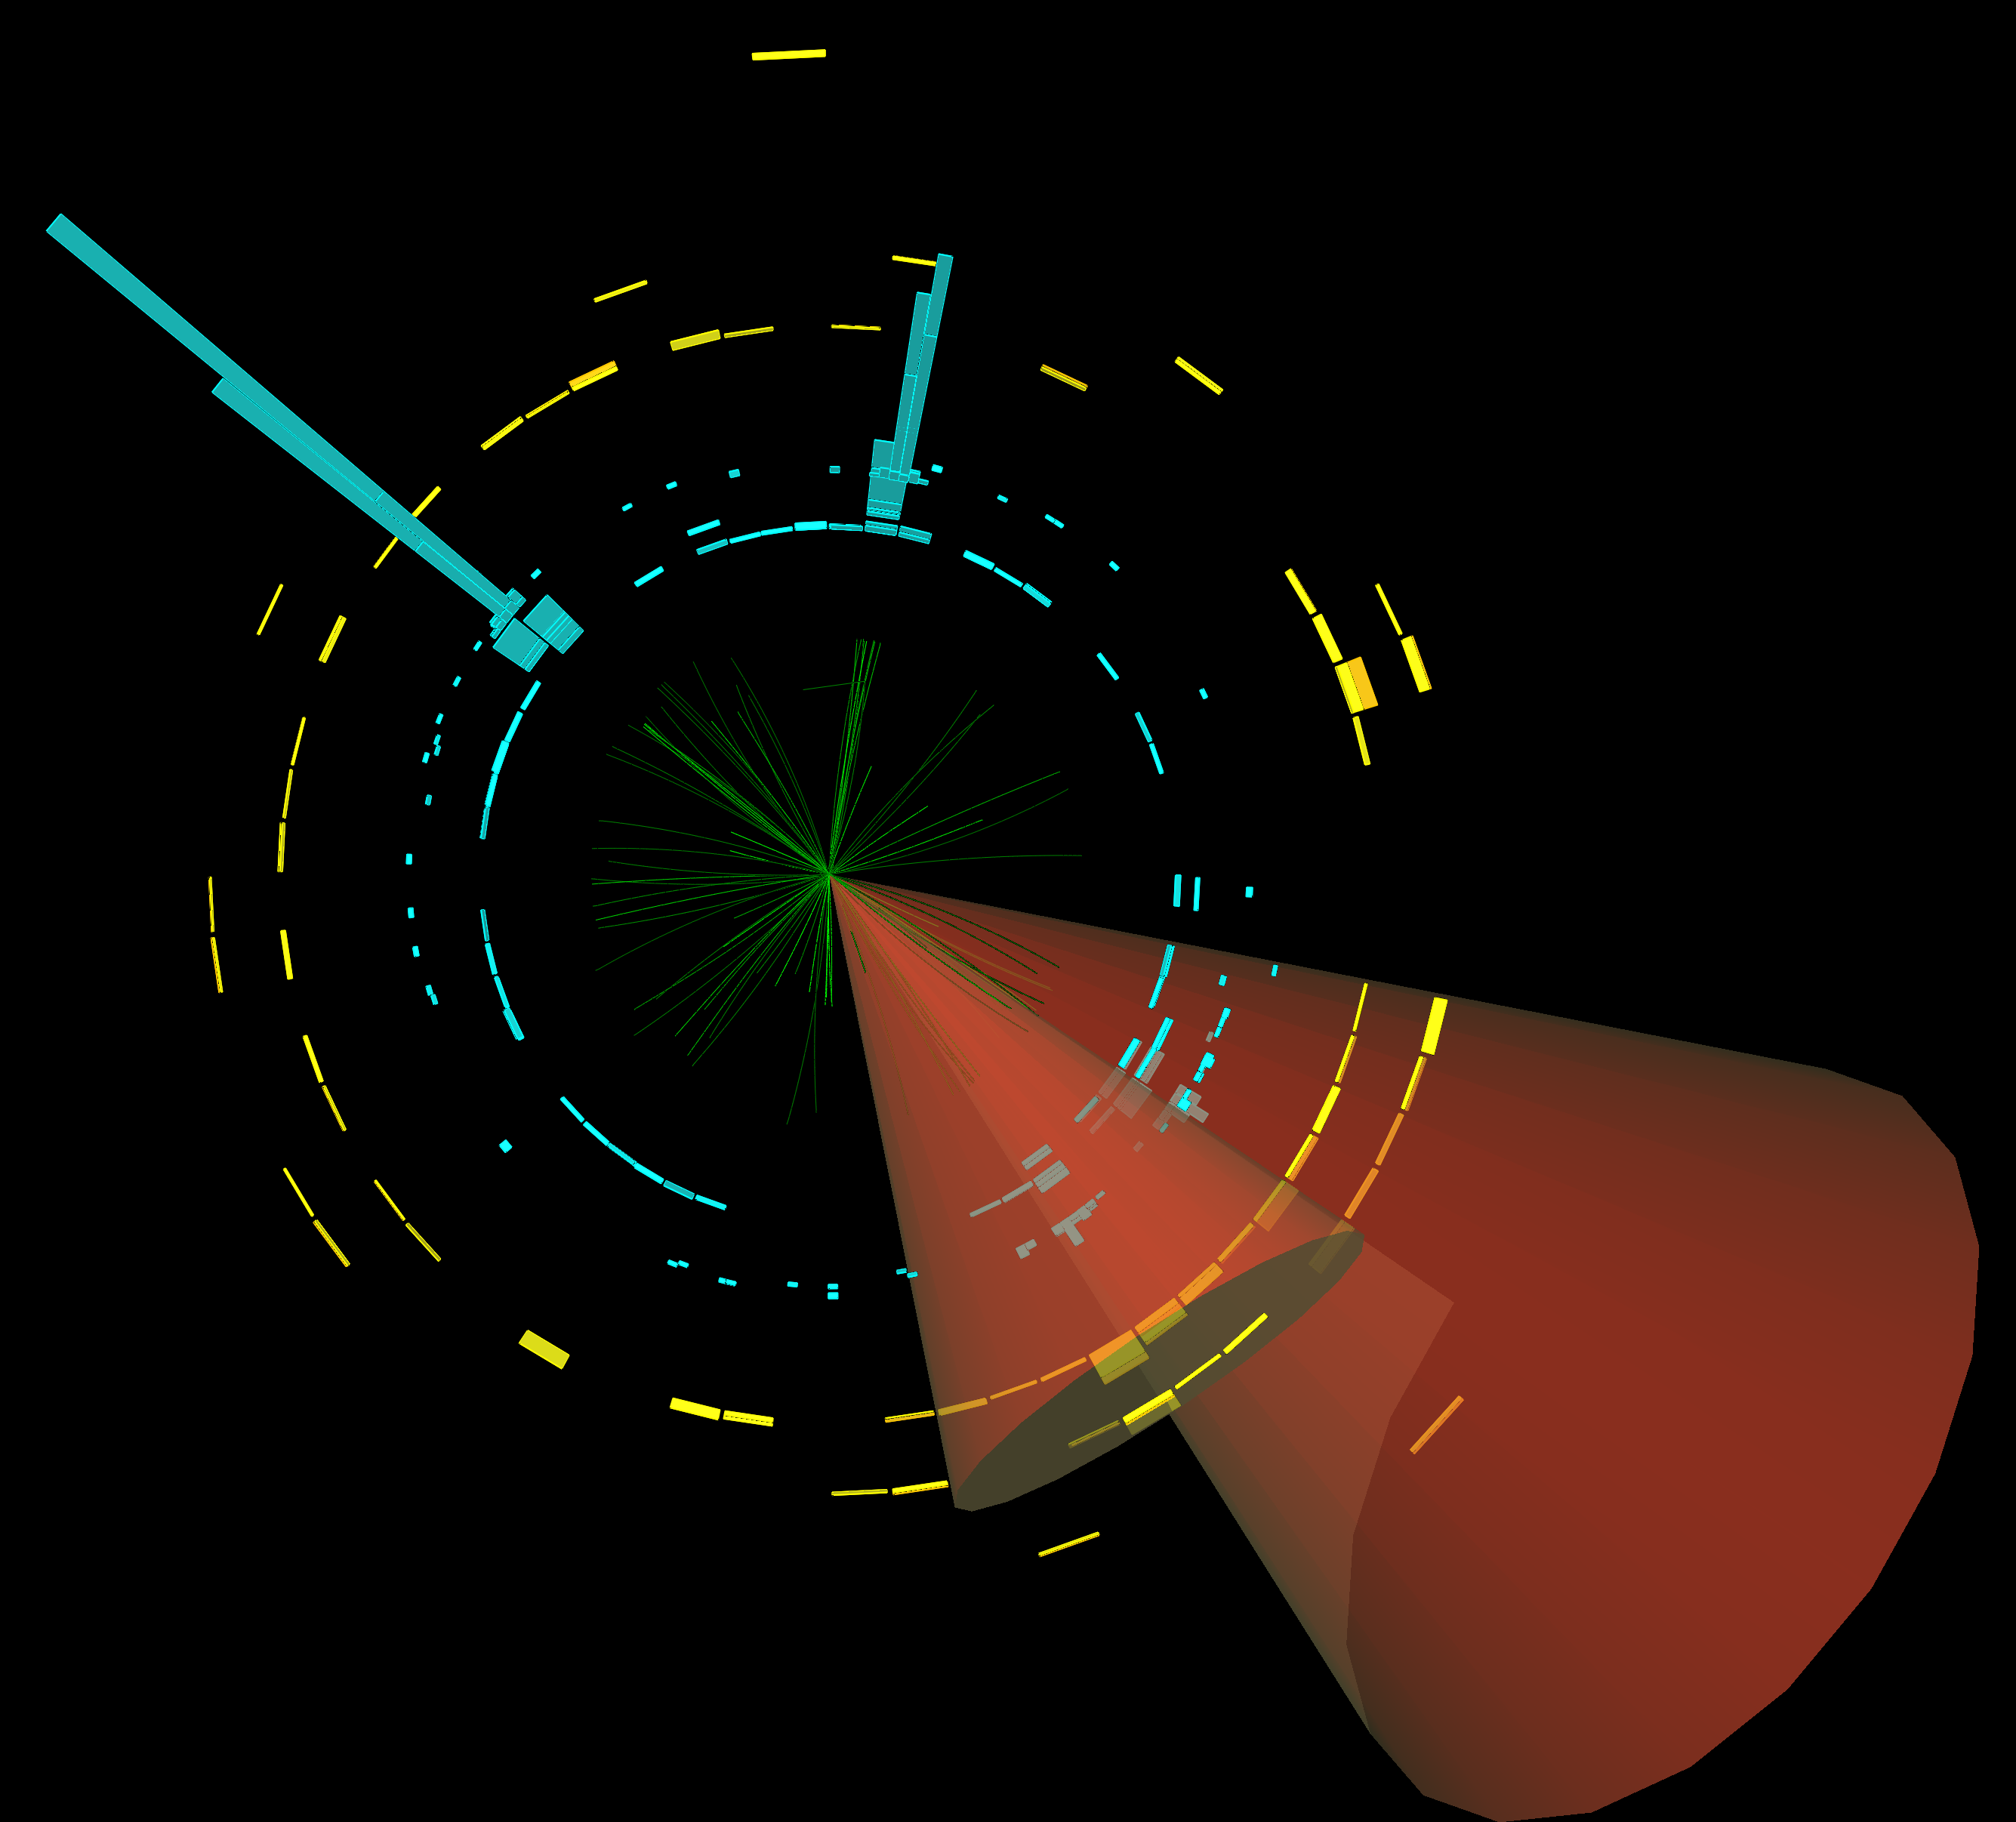
\includegraphics[width=1.05\paperwidth]{Img/figaux_02}}
\begin{frame}
\titlepage
\end{frame}
}

\section*{Content}
\begin{frame}{Content}
\label{content}
    \begin{columns}[t]
        \begin{column}{.5\textwidth}
            \tableofcontents[sections={1-5}]
        \end{column}
        \begin{column}{.5\textwidth}
            \tableofcontents[sections={6-}]
        \end{column}
    \end{columns}
    %\tableofcontents
\end{frame}

\section{Theoretical framework}
\begin{frame}{Content}
\label{content}
    \begin{columns}[t]
        \begin{column}{.5\textwidth}
            \tableofcontents[sections={1-5},currentsection]
        \end{column}
        \begin{column}{.5\textwidth}
            \tableofcontents[sections={6-},currentsection]
        \end{column}
    \end{columns}
\end{frame}
\subsection{The Standard Model of particle physics}

\begin{frame}{The Standard Model (SM) of particle physics}

%\begin{textblock*}{5cm}(13.2cm, 3.cm) % {block width} (coords) 
%   \textbf{\textcolor{HHturquoise_d}{Strong}}
%\end{textblock*}
%\begin{textblock*}{5cm}(13.2cm, 4.2cm) % {block width} (coords) 
%   \textbf{\textcolor{HHturquoise_m}{Electromagnetic}}
%\end{textblock*}
%\begin{textblock*}{5cm}(13.2cm, 5.4cm) % {block width} (coords) 
%   \textbf{\textcolor{HHturquoise_m}{Weak}}
%\end{textblock*}

\begin{columns}
\column{0.5\textwidth}

\begin{itemize}
    \item Quantum field theory, based on the principal gauge invariance $\textcolor{HHturquoise_d}{SU(3)}\times \textcolor{HHred}{SU(2)}\times \textcolor{HHturquoise_m}{U(1)}$
    \item Unify \textbf{\textcolor{HHturquoise_d}{Strong}} and \textbf{\textcolor{HHturquoise_m}{Electro}-\textcolor{HHred}{weak}} interactions
    \item \textbf{Fermions}: matter particles
    \begin{itemize}
        \item \textbf{\textcolor{violet}{Quarks}}
        \item \textbf{\textcolor{applegreen}{Leptons}}
    \end{itemize}
    \item \textbf{\textcolor{cadmiumorange}{Gauge bosons}}: mediators of interactions
\end{itemize}    
\begin{itemize}    
    \item \textbf{\textcolor{HHyellow}{Higgs boson}}: responsible for mass generation through EWSB mechanism
    
\end{itemize}

\column{0.5\textwidth}
\begin{figure}
    \centering
    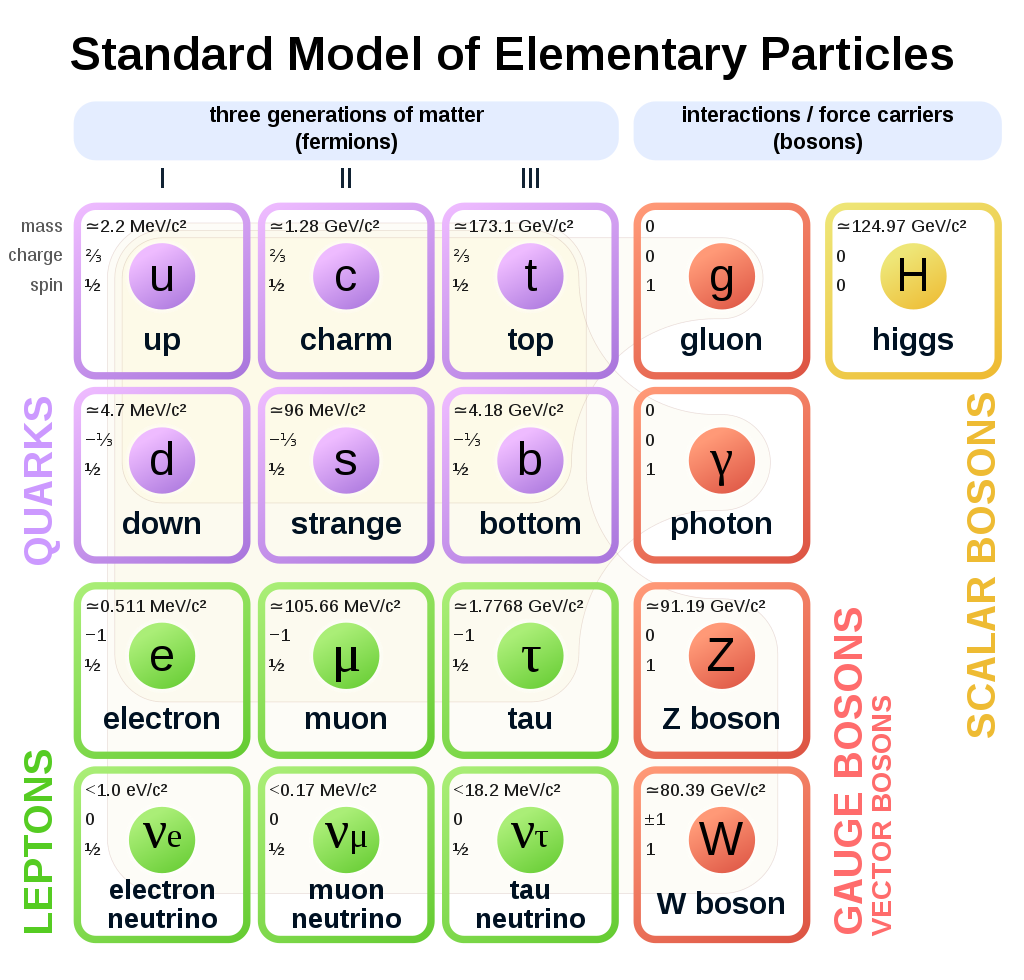
\includegraphics[width=1\textwidth]{Part1/Img/SM_particles.png}
\end{figure}
\end{columns}
\end{frame}

\begin{frame}{Electroweak Symmetry Breaking and Higgs boson}
\setbeamercovered{transparent}
\begin{textblock*}{5cm}(12.2cm, 6.5cm) % {block width} (coords) 
\visible<2>{
\begin{figure}
    \begin{overprint}
    \centering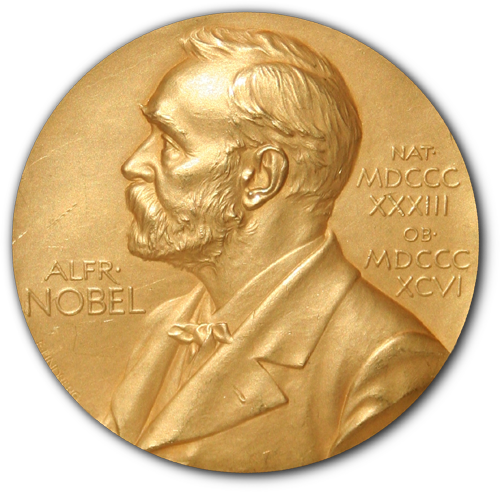
\includegraphics[width=0.2\textwidth]{Part1/Img/Nobel_Prize.png}
    \end{overprint}
\end{figure}
}
\end{textblock*}
\begin{textblock*}{5cm}(10cm, 3.9cm) % {block width} (coords) 
$\mu^2 <$ 0 $\to$ Mexican hat 
\end{textblock*}
\begin{columns}
\column{0.4\textwidth}
\begin{figure}
    \centering
    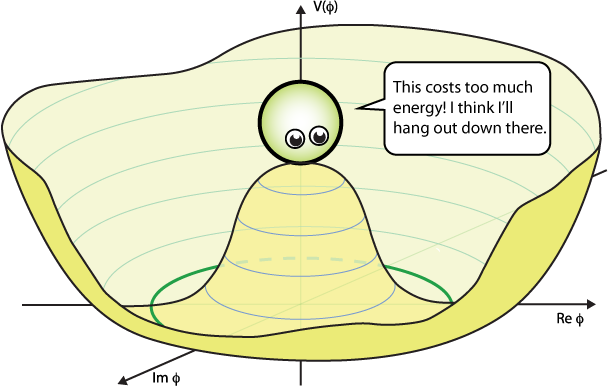
\includegraphics[width=0.8\textwidth]{Part1/Img/Higgs-Potential-lookdown.png}
\end{figure}
\visible<2>{
\begin{figure}
    \centering
    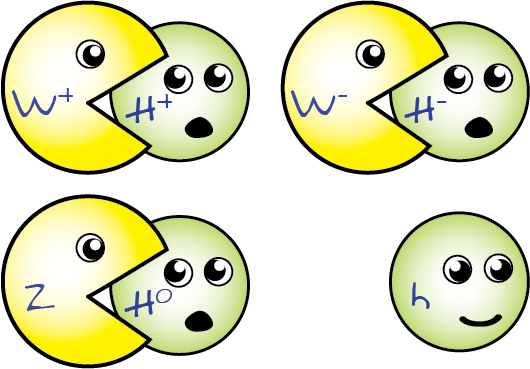
\includegraphics[width=0.8\textwidth]{Part1/Img/Goldstone-Eaten-four.png}
\end{figure}
}
\column{0.6\textwidth}
Gauge boson mass terms break gauge symmetry of SM
\begin{itemize}
    \item \textcolor{structurColor}{Brout-Englert-Higgs (1964)} include complex scalar field
    \begin{equation*}
        V(\phi^\dagger\phi) = \mu^2\phi^\dagger\phi + \lambda(\phi^\dagger\phi)^2
    \end{equation*}
    \pause
    \item Choice of the vacuum state $v$ \textbf{\textcolor{applegreen}{spontaneously breaks the symmetry}}
    \begin{itemize}
        \item Gauge bosons become massive
        \item \textbf{Higgs boson}: $m_{H}= -2\mu^2$
        \item Fermion masses: generated through Yukawa couplings
    \end{itemize}
\end{itemize}

\begin{itemize}
    \item \underline{Observed} in 2012 at LHC, $m_{H} \sim $ 125 GeV
\end{itemize}
\end{columns}
\end{frame}

\begin{frame}{Measurements of Higgs parameters}

\begin{textblock*}{5cm}(2.5cm,3.2cm) % {block width} (coords) 
   \textcolor{HHturquoise_d}{\textbf{mass}}
\end{textblock*}
\begin{textblock*}{5cm}(2cm,6.7cm) % {block width} (coords) 
   \textcolor{HHred}{\small\textbf{125.09 $\pm$ 0.24 GeV}}
\end{textblock*}

\begin{textblock*}{5cm}(7.6cm,3.2cm) % {block width} (coords) 
   \textcolor{HHturquoise_d}{\textbf{cross-section}}
\end{textblock*}
\begin{textblock*}{5cm}(12.5cm,2cm) % {block width} (coords) 
   \textcolor{HHturquoise_d}{\textbf{coupling}}
\end{textblock*}

\begin{textblock*}{5cm}(12.5cm,4cm) % {block width} (coords) 
   \small\textbf{$\sim$20\%}
\end{textblock*}

\begin{textblock*}{5cm}(14.3cm,3.2cm) % {block width} (coords) 
   \small\textbf{$<$10\%}
\end{textblock*}


\begin{figure}
    \centering
      \subfloat{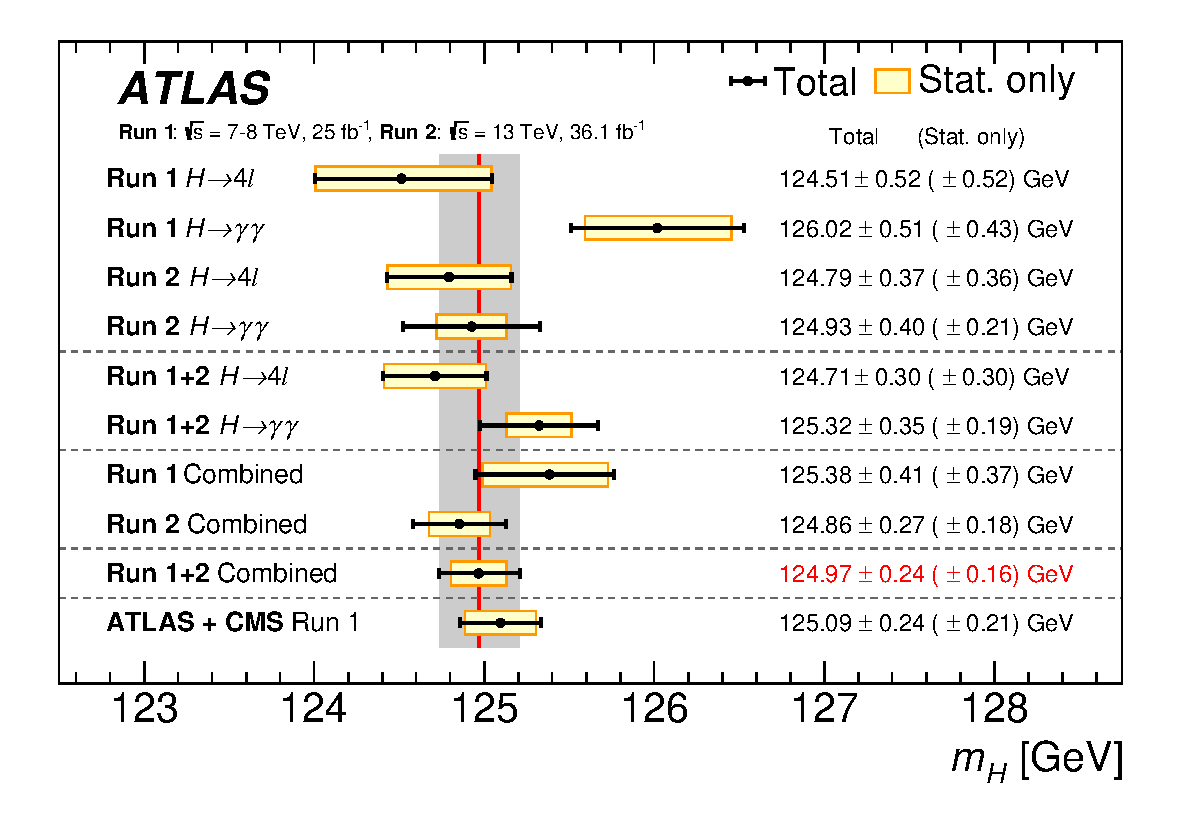
\includegraphics[width=0.35\textwidth]{Part1/Img/ATLAS_HIGGS1100_mass_Summary.pdf}}
      \subfloat{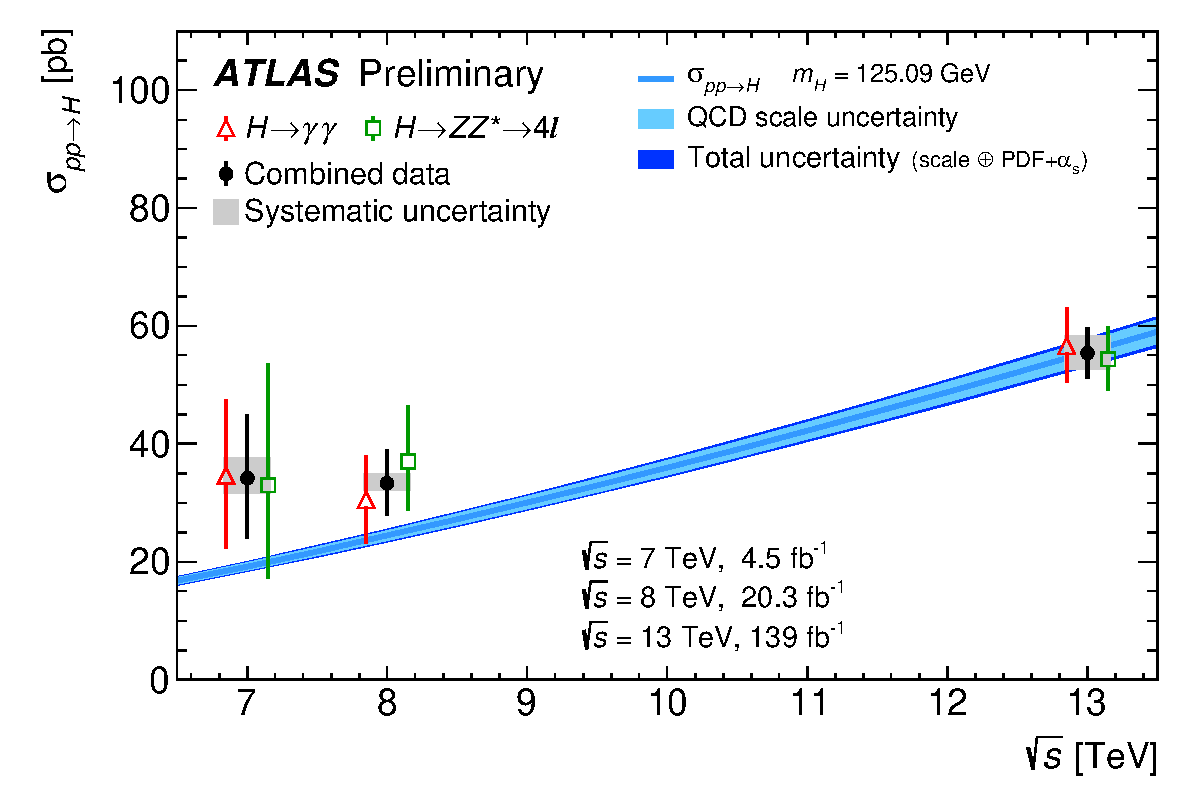
\includegraphics[width=0.35\textwidth]{Part1/Img/ATLAS_HIGGS3010_XSvsCME_Summary.pdf}}
%    \subfloat{ 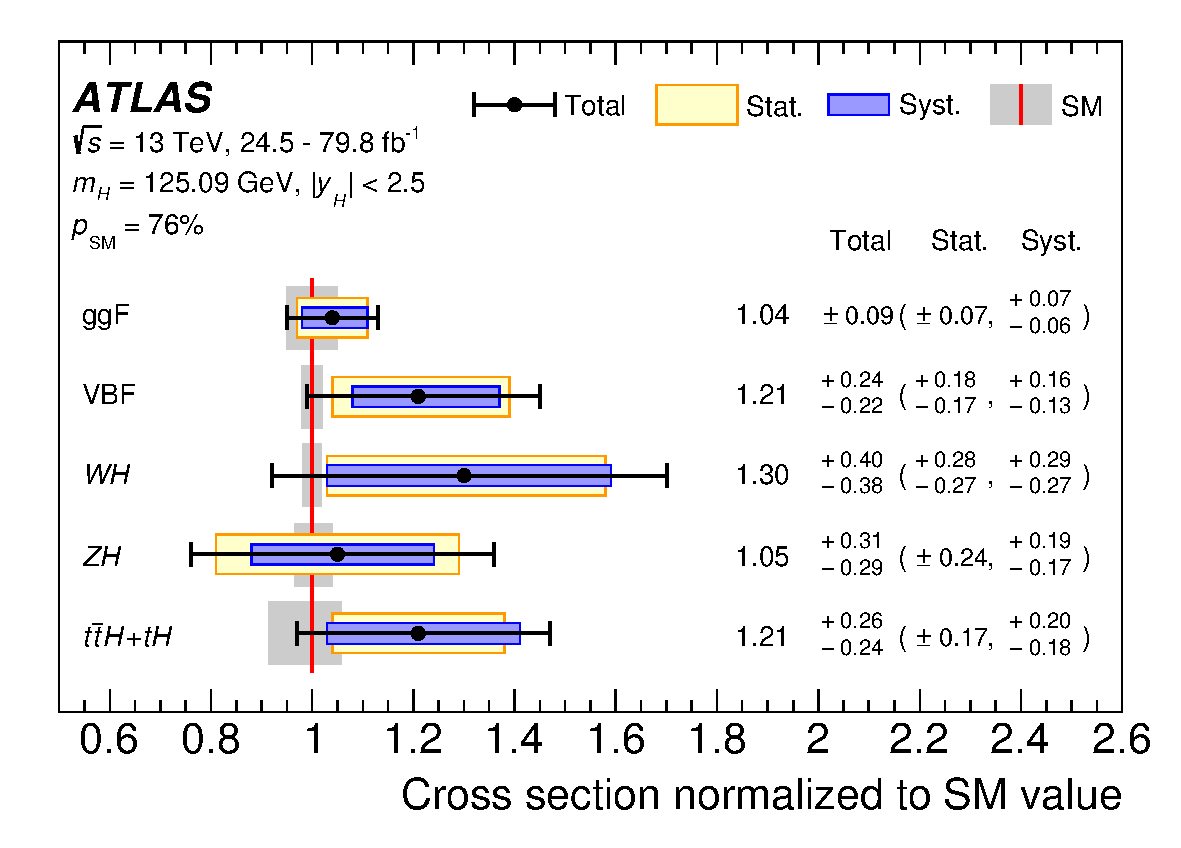
\includegraphics[width=0.5\textwidth]{Part1/Img/ATLAS_HIGGS3250_Run2XS_Summary.pdf}}
      \subfloat{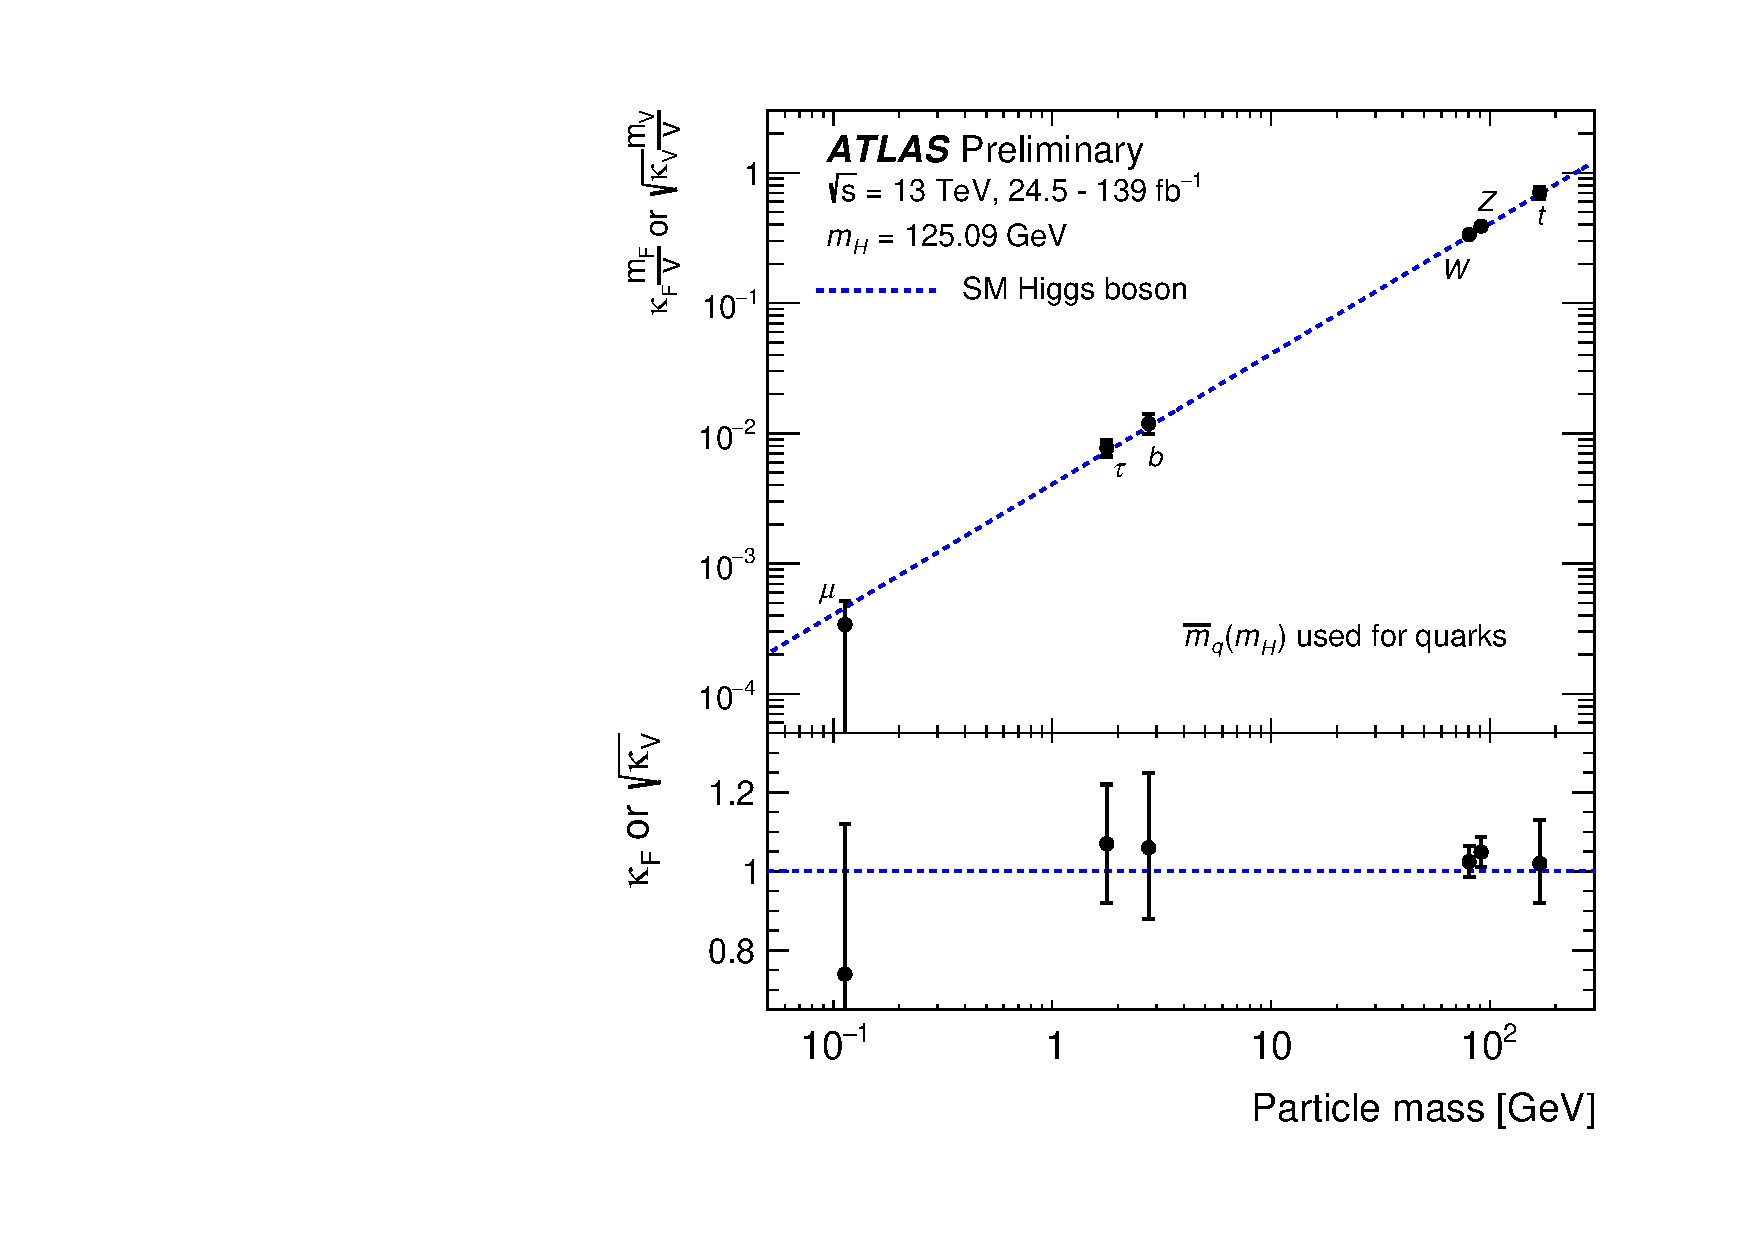
\includegraphics[width=0.35\textwidth]{Part1/Img/ATLAS_HIGGS4400_kappa_vs_mass.pdf}}
\end{figure}

\begin{itemize}
    \onslide<2>{
    \item \textcolor{HHred}{Not all, Higgs boson self-coupling still resists to physicists}
    }
\end{itemize}

\end{frame}

\subsection{Higgs boson self-coupling}

\begin{frame}{Higgs boson self-coupling}
\begin{columns}
\column{0.6\textwidth}    
\begin{itemize}
    \item \textbf{Self-coupling: \textcolor{structurColor}{Higgs boson trilinear coupling}}
    \item Controls the shape of the Higgs potential
    \begin{itemize}
        \item It is important to measure both $m_{H}$ and $\lambda$
    \end{itemize}
    \item \textbf{B}eyond \textbf{SM} (BSM) physics would impact this coupling, impact quantified as
    \begin{equation*}
       \textcolor{HHred}{\kappa_{\lambda} = \frac{\lambda}{\lambda^{SM}}}
    \end{equation*}
    \onslide<3>{
    \item Measured \underline{\textbf{directly}} with \textbf{\textcolor{HHturquoise_d}{Higgs boson pair (\textbf{HH}) production}} 
    }
\end{itemize}

\column{0.4\textwidth}  

\begin{textblock*}{5cm}(13cm,6.2cm) % {block width} (coords) 
  \visible<1>{ not accessible \\ at LHC }
\end{textblock*}

\begin{textblock*}{5cm}(14.5cm,4.2cm) % {block width} (coords) 
  \visible<2>{\textcolor{HHturquoise_d}{$\lambda=1$}} \\
  \visible<2>{\textcolor{applegreen}{$\lambda=0$}} \\
  \visible<2>{\textcolor{violet}{$\lambda=-1$}}
\end{textblock*}
\begin{equation*}
    V \supset \frac{m_{H}^2}{2}H^2 + \textcolor{HHred}{\lambda} vH^3 + \frac{\textcolor{HHred}{\lambda}}{v}H^4
\end{equation*}
\begin{equation*}
    \lambda^{SM} = \frac{m_{H}^2}{2v^2} \sim 0.13
\end{equation*}

\begin{figure}
    \begin{overprint}
    \onslide<1>\centering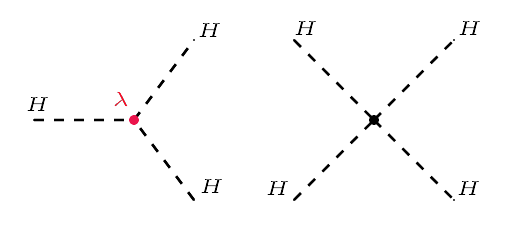
\includegraphics[width=0.9\textwidth]{Part1/Img/hhh_diagrams.png}
    \onslide<2>\centering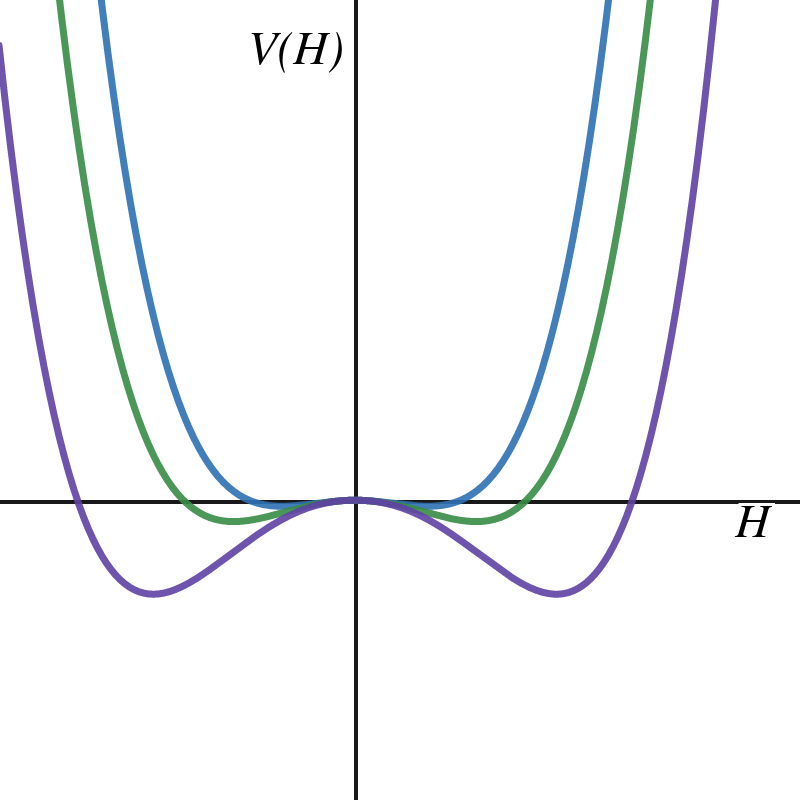
\includegraphics[width=0.8\textwidth]{Part1/Img/V_H_for_lambda.png}
    \onslide<3>\centering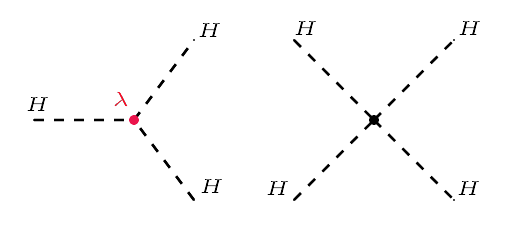
\includegraphics[width=0.9\textwidth]{Part1/Img/hhh_diagrams.png}
    \end{overprint}
\end{figure}

\end{columns}    

\end{frame}

\subsection{Higgs boson pair production}

\begin{frame}{Higgs boson pair production at the LHC}
\begin{textblock*}{5cm}(5.8cm, 1.8cm) % {block width} (coords) 
  \textcolor{black}{\textbf{Destructive interference}}
\end{textblock*}

\begin{textblock*}{5cm}(6.4cm, 2.5cm) % {block width} (coords) 
  \textcolor{black}{$\kappa_t$}
\end{textblock*}

\begin{itemize}
    \item Produced mainly via \textbf{\underline{non-resonant}} \textbf{\textcolor{HHred}{gluon-gluon Fusion}} \textbf{(ggF)} and \textbf{\textcolor{HHturquoise_d}{Vector Boson Fusion}} \textbf{(VBF)}
\end{itemize}

\begin{figure}
    \fcolorbox{HHred}{HHwhite2}{     \subfloat{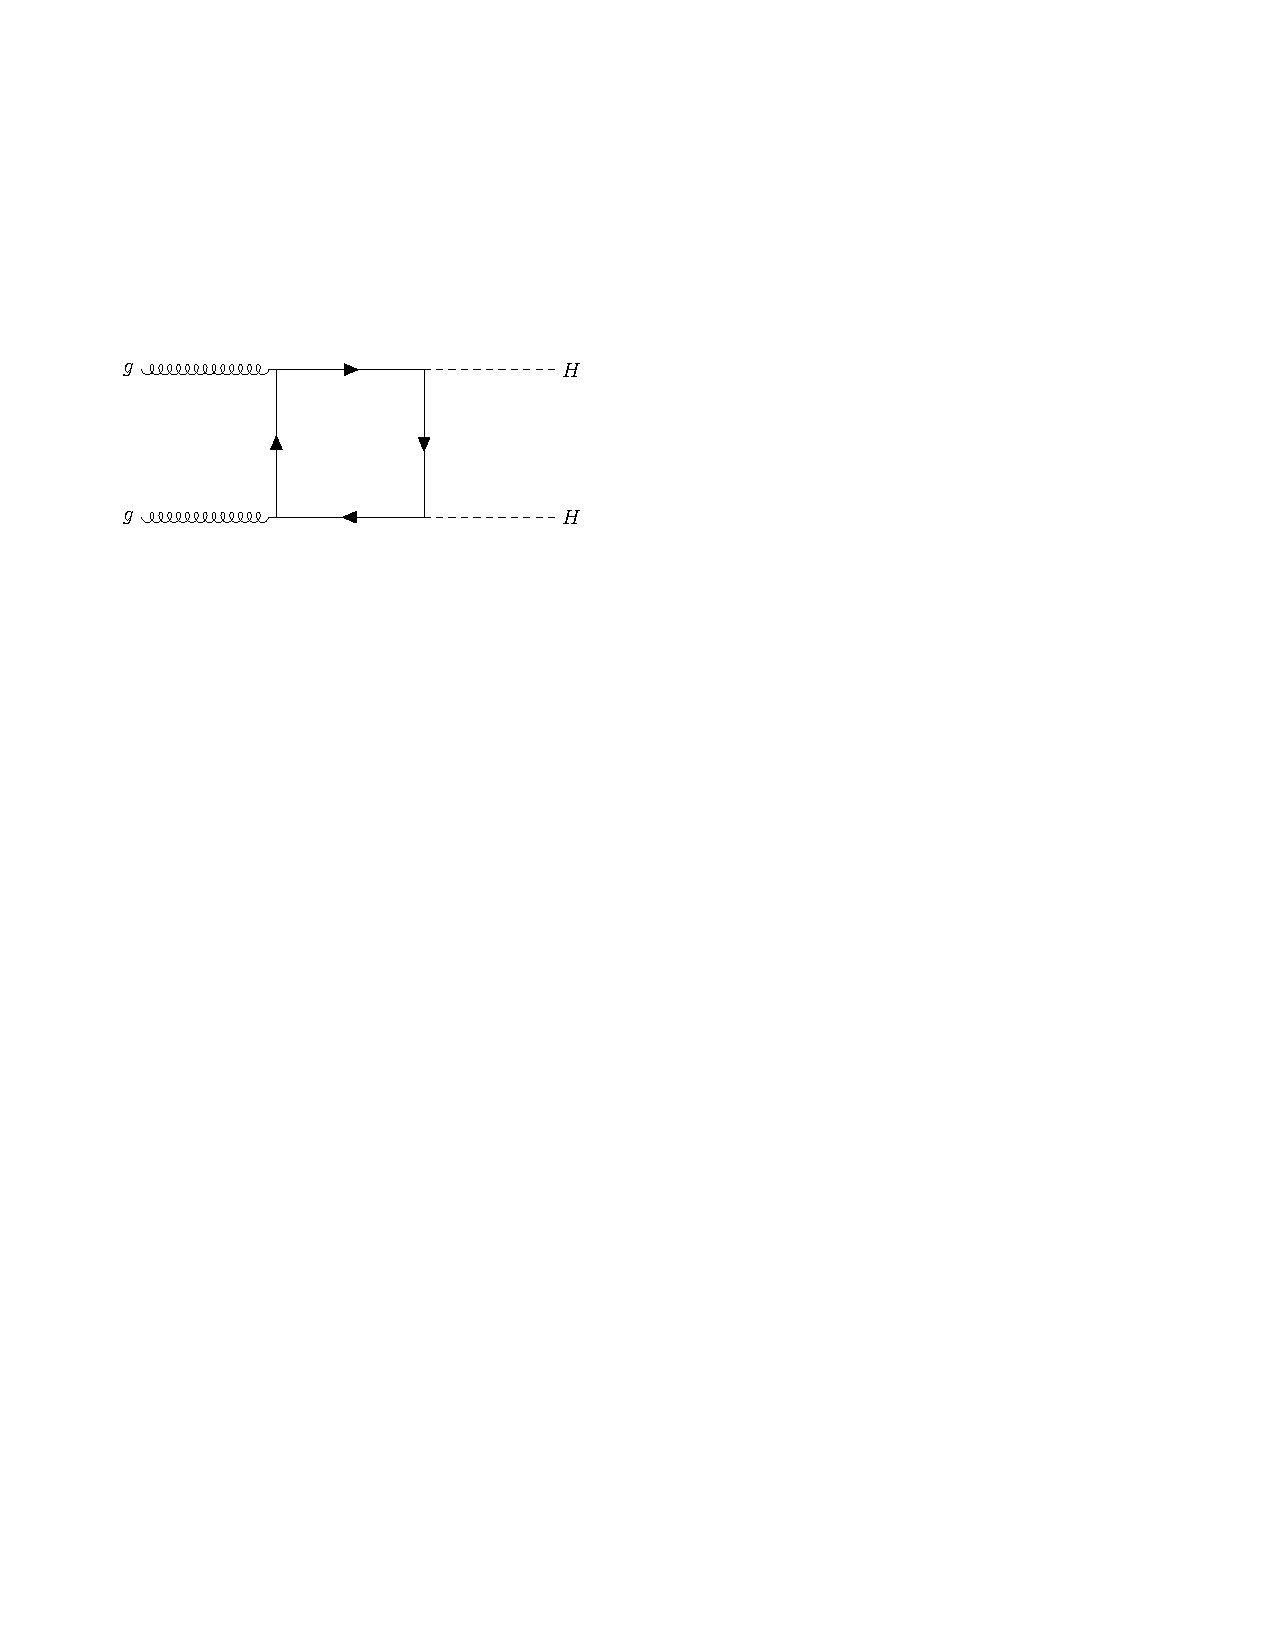
\includegraphics[width=0.3\textwidth]{Part1/Img/ggF_box.pdf}}
    \subfloat{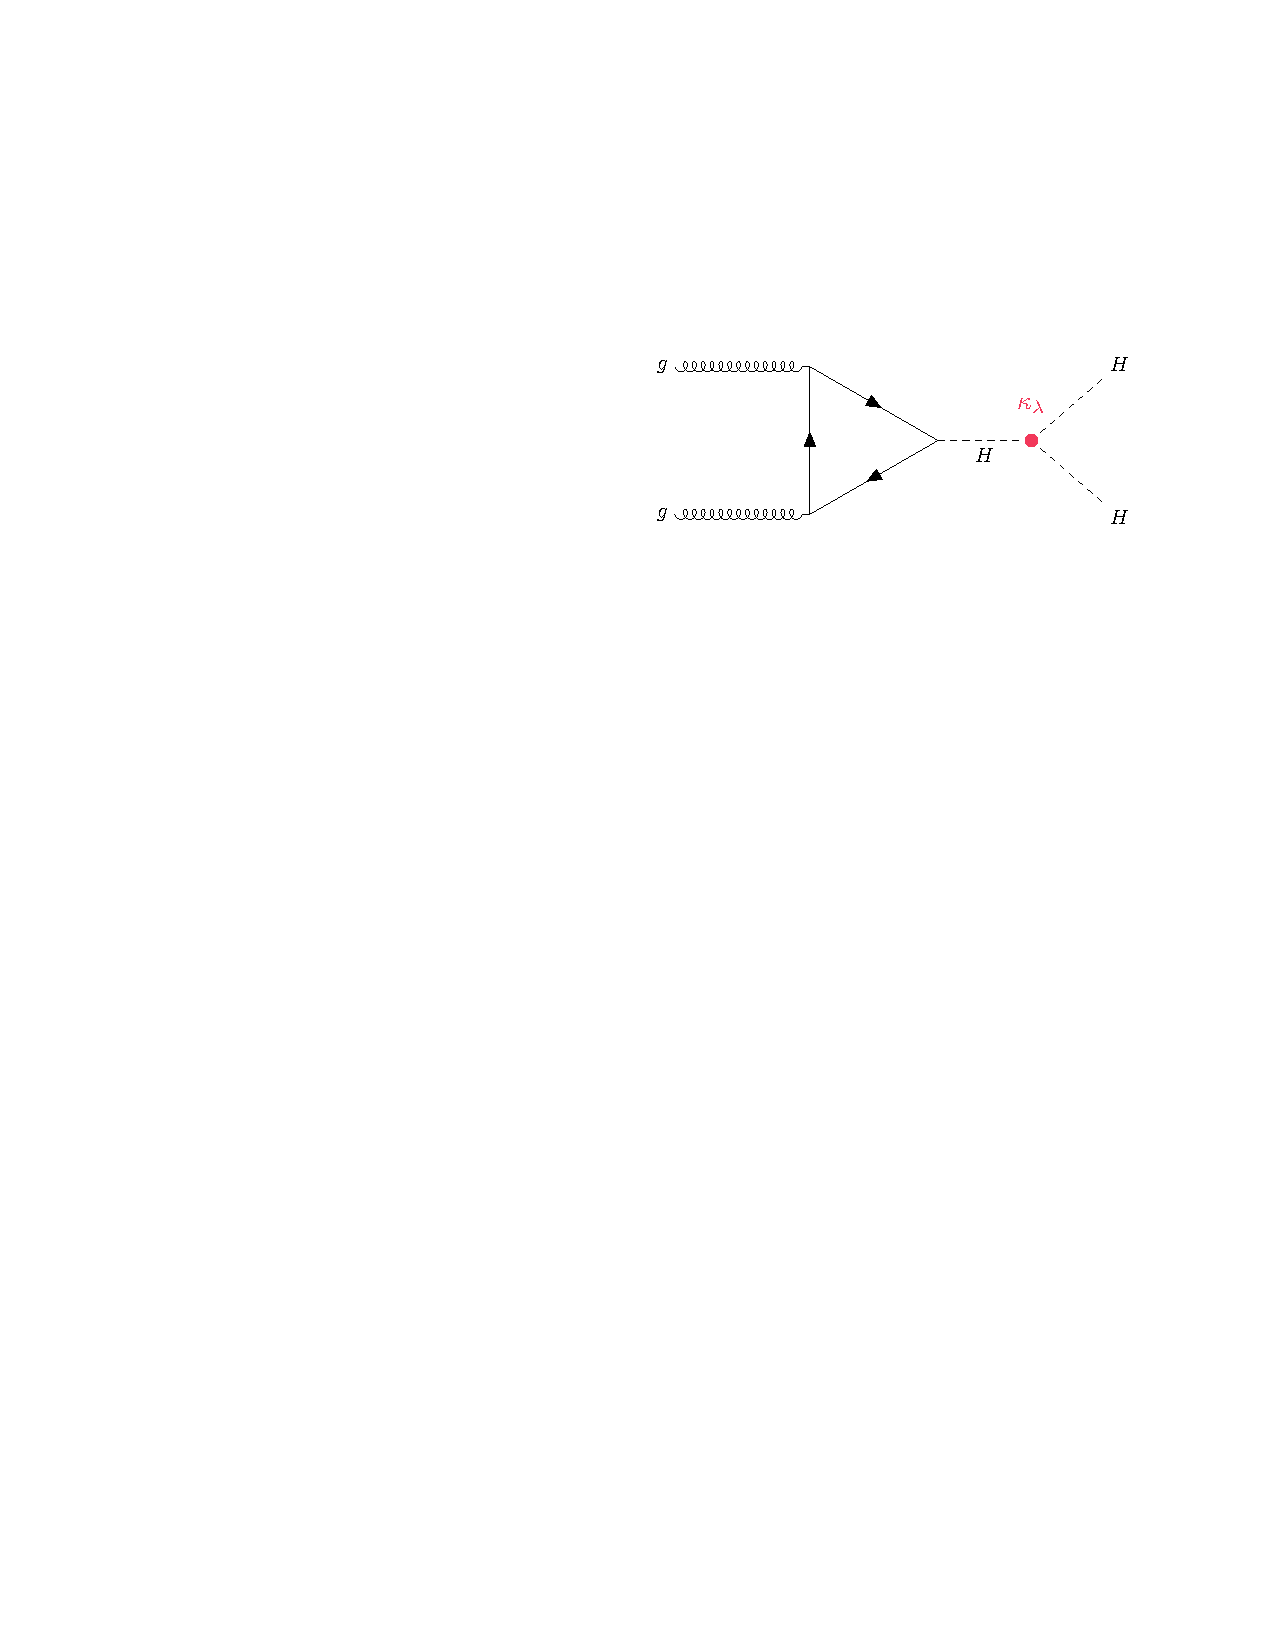
\includegraphics[width=0.3\textwidth]{Part1/Img/ggF_tri.pdf}}} \\
    \fcolorbox{HHturquoise_d}{HHwhite2}{
    \subfloat{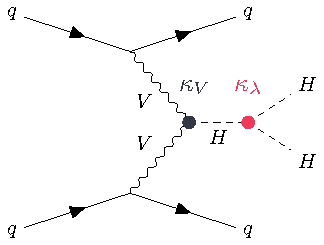
\includegraphics[width=0.2\textwidth]{Part1/Img/VBF_kvkl.pdf}}
    \subfloat{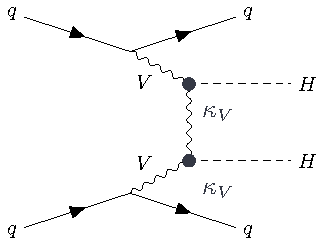
\includegraphics[width=0.2\textwidth]{Part1/Img/VBF_kvkv.pdf}}
    \subfloat{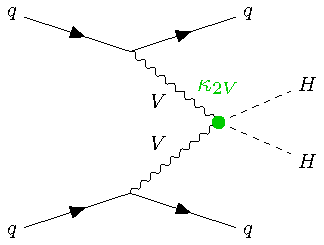
\includegraphics[width=0.2\textwidth]{Part1/Img/VBF_k2v.pdf}}
    }
\end{figure}

\begin{itemize}
    \item At 13 TeV, $m_{H} = $ 125.09 GeV and $\kappa_{\lambda} = $ 1 
    \begin{itemize}
        \item \textcolor{HHred}{\textbf{$\sigma^{ggF}_{HH} = $ 31.02 fb}}, 3 order of magnitude smaller than $\sigma_{H}$
        \item \textcolor{HHturquoise_d}{\textbf{$\sigma^{VBF}_{HH} = $ 1.72 fb}}, one order of magnitude more smaller than ggF
    \end{itemize}
\end{itemize}

\end{frame}

\begin{frame}{Di-Higgs boson as a probe of BSM physics}

\begin{columns}
\column{0.6\textwidth} 
\begin{itemize}
    \item Low cross-section, BSM anomaly may enhance it
    \item BSM physics could manifest as deviations
    \begin{itemize}
        \item \textbf{\textcolor{HHred}{Total}} production rate
        \item \textbf{\textcolor{HHturquoise_m}{Kinematic}} of HH event
    \end{itemize}
    \item Measurement of $\kappa_{\lambda}$ $\to$ \textbf{$\kappa_{\lambda} \neq $ 1}, presence of \textbf{new physics} 
\end{itemize}
%\onslide<2>{
%\underline{Thesis aim}: \textbf{search for HH events in the $b \bar{b}\gamma\gamma$ final state and constrain $\kappa_{\lambda}$}
%}
\column{0.4\textwidth}  
%\begin{textblock*}{5cm}(13cm,5.8cm) % {block width} (coords) 
%  \textcolor{HHred}{\textbf{Destructive \\ interference}}
%\end{textblock*}
%\begin{figure}
%    \centering
%    \fcolorbox{HHred}{HHwhite2}{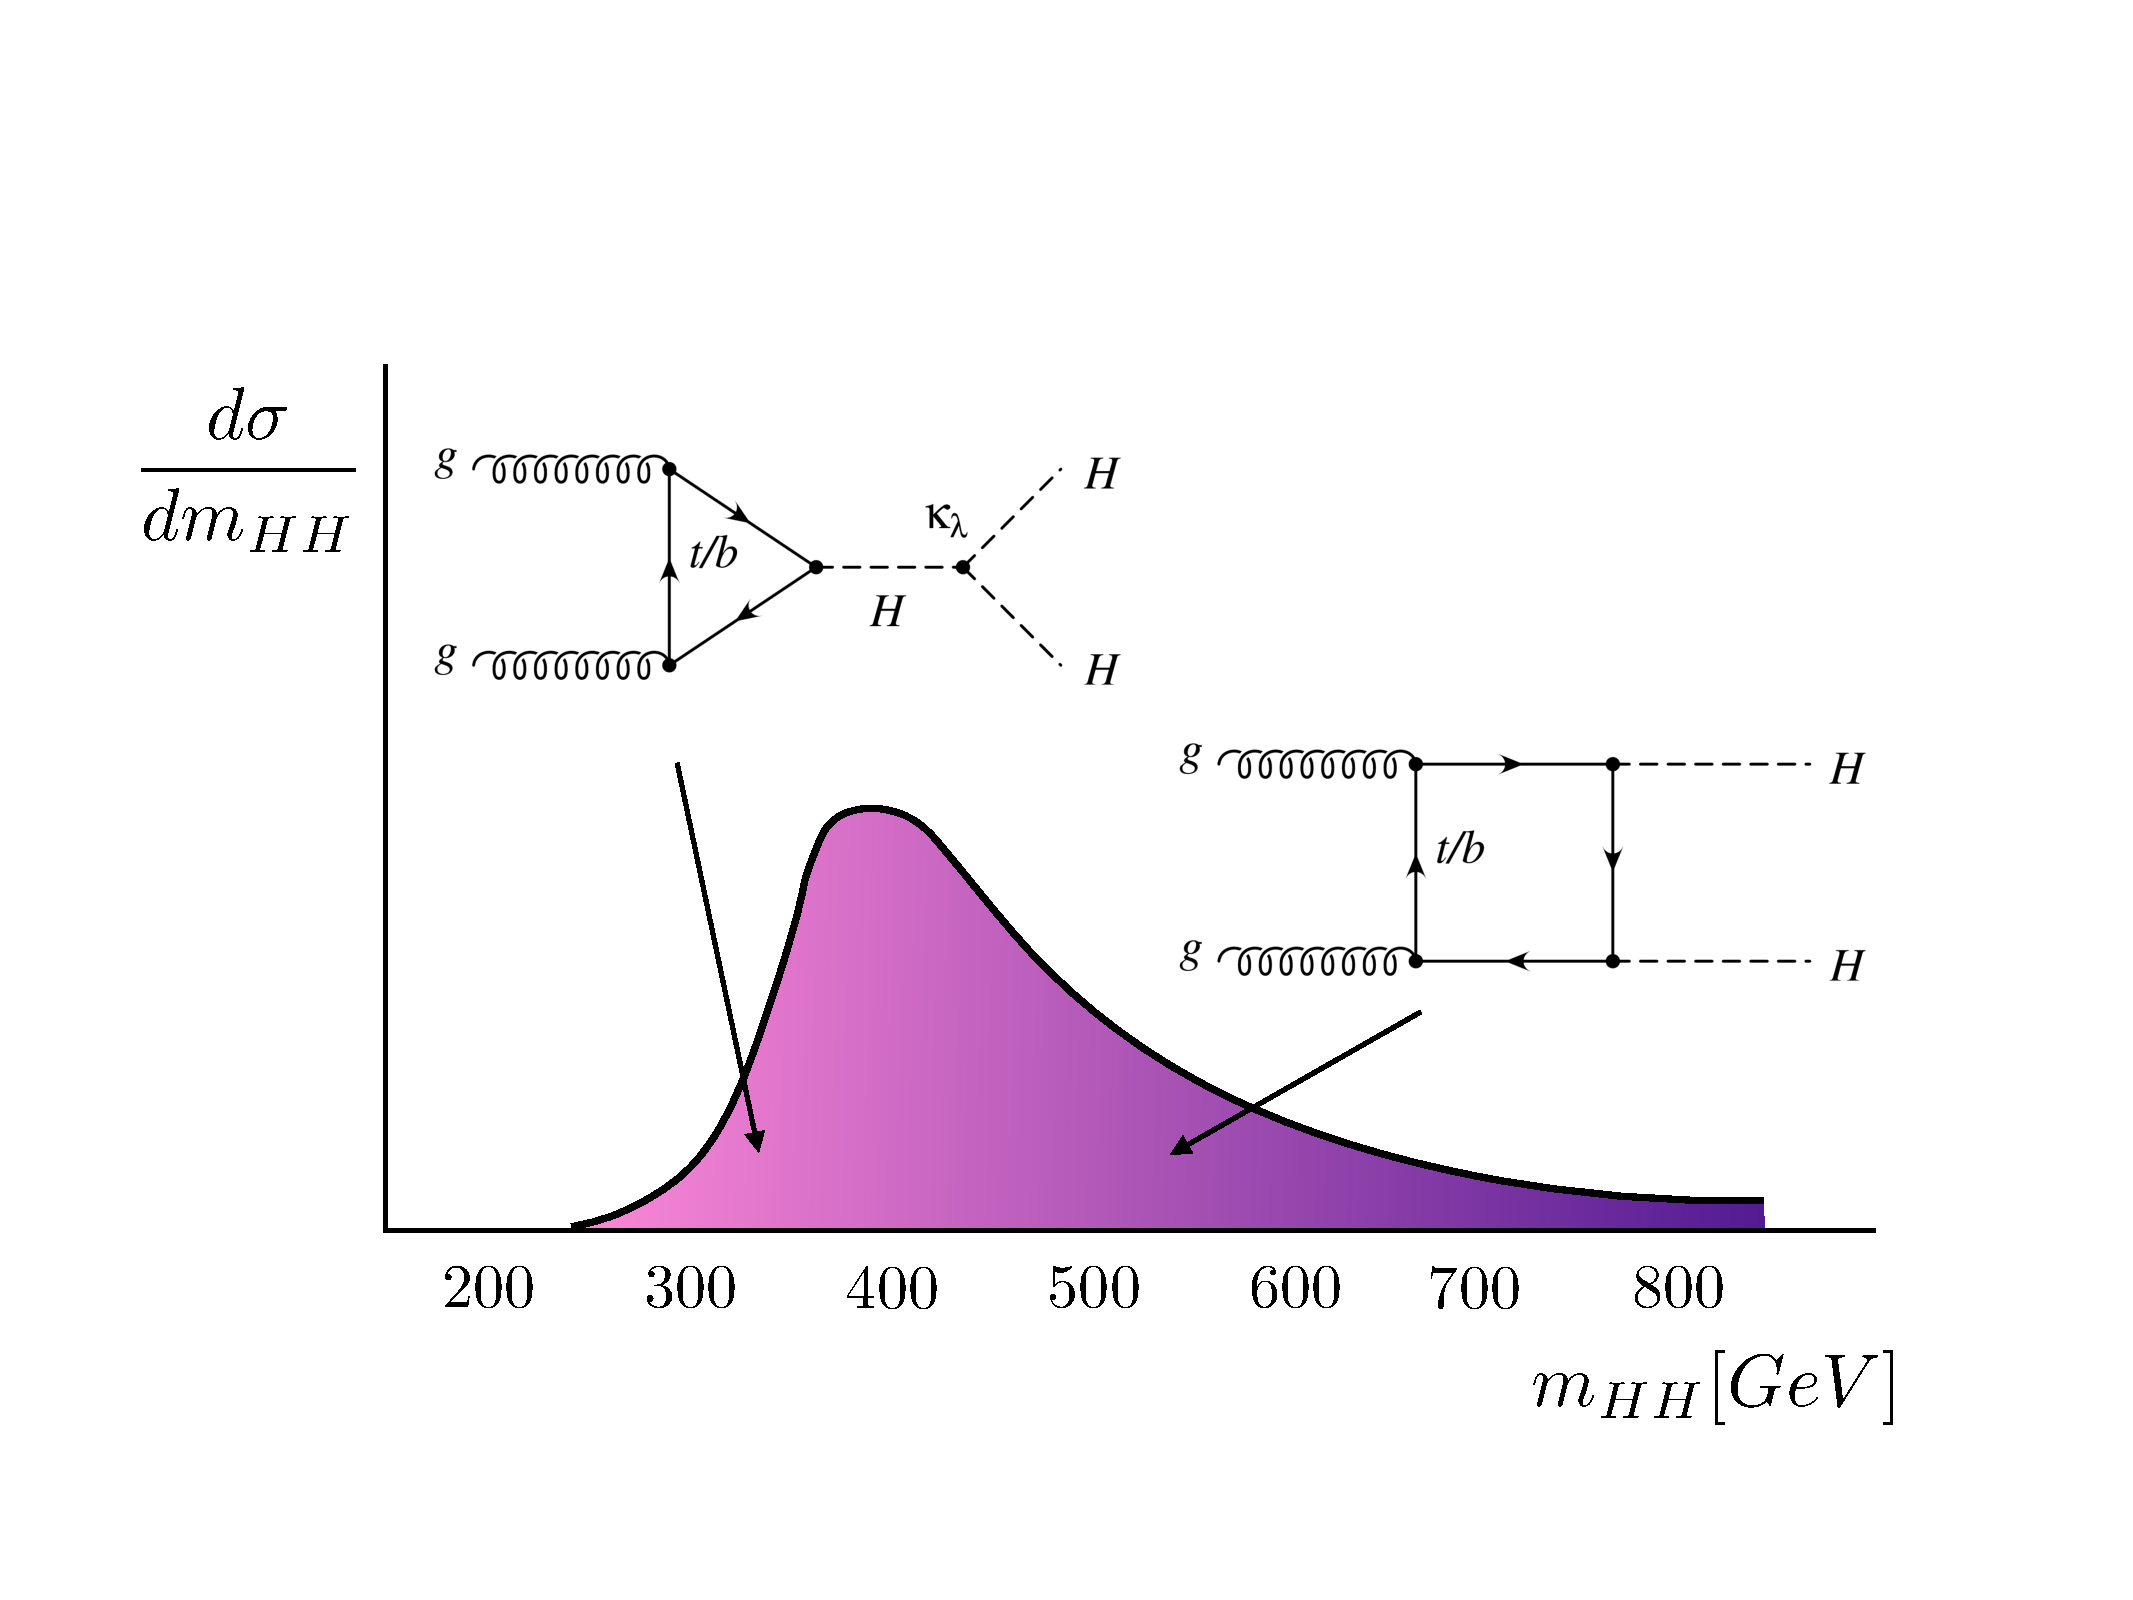
\includegraphics[width=0.7\textwidth]{Part1/Img/mHHSketch.pdf}}
%\end{figure}

\begin{figure}
    \begin{overprint}
    \onslide<1>\centering\fcolorbox{HHred}{HHwhite2}{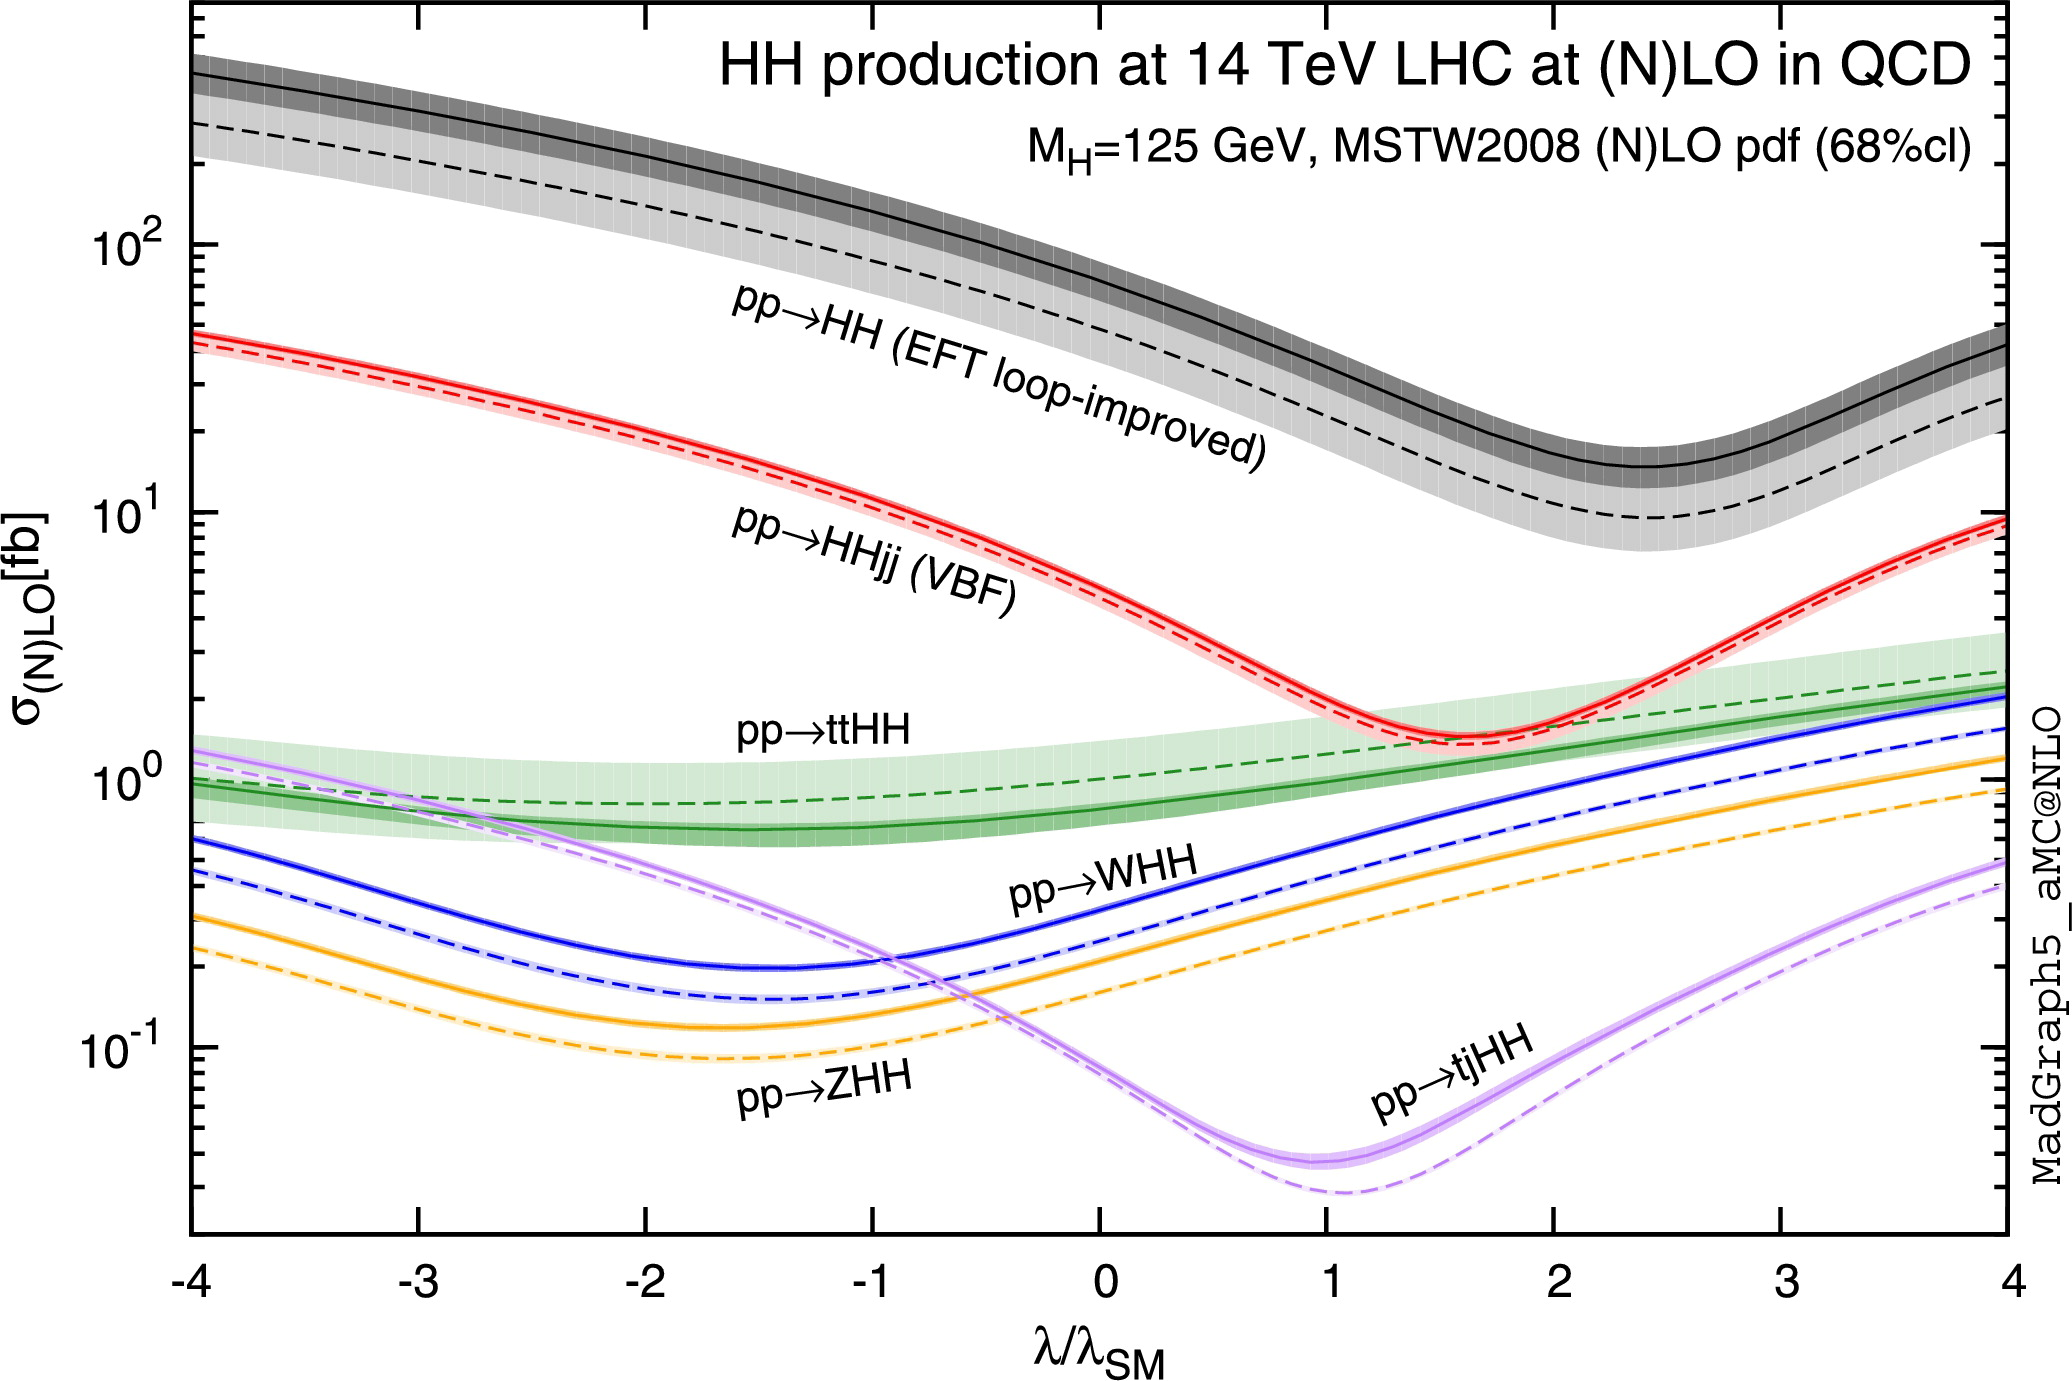
\includegraphics[width=1\textwidth]{Part1/Img/HH_xsec_lambda.jpg}}
    \onslide<2->\centering\fcolorbox{HHturquoise_m}{HHwhite2}{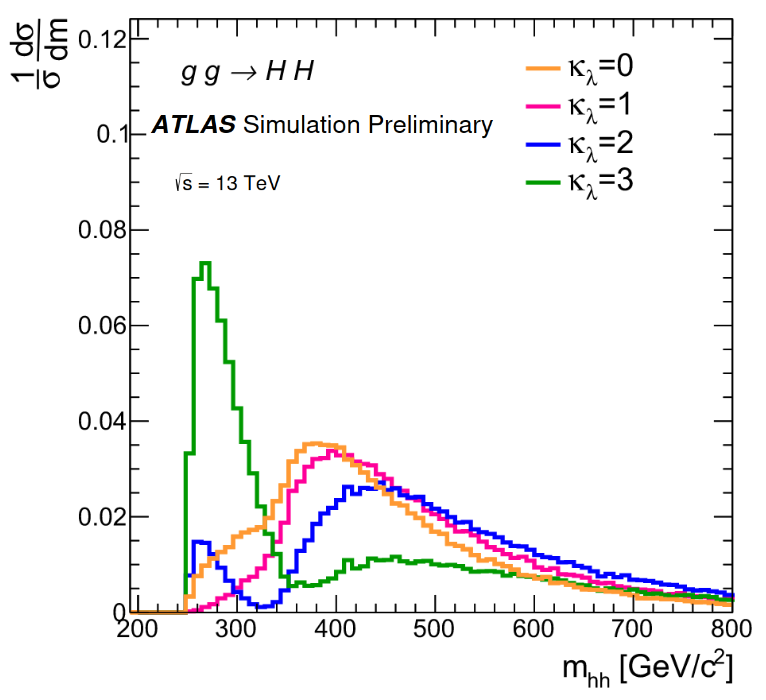
\includegraphics[width=0.9\textwidth]{Part1/Img/mHH.png}}
    \end{overprint}
\end{figure}

\end{columns}
\end{frame}

\begin{frame}{Di-Higgs boson decay modes}
\begin{textblock*}{5cm}(6.75cm, 5.2cm) % {block width} (coords) 
  \textcolor{HHred}{\textbf{$\star$}}
\end{textblock*}

\begin{figure}
    \centering
    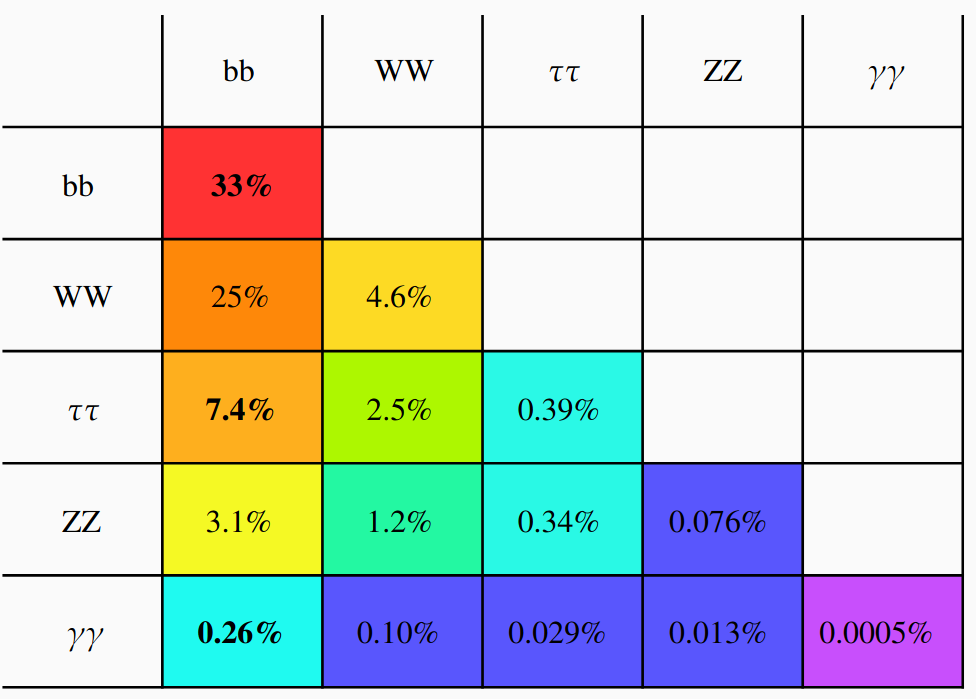
\includegraphics[width=0.43\textwidth]{Part1/Img/HH_decays2.png}
\end{figure}
\pause
\begin{itemize}
    \item \textbf{\textcolor{HHred}{Focusing on H($\to b\bar{b}$)H($\to\gamma\gamma$)}}
    \item Despite low decay rate, competitive channel
    \begin{itemize}
        \item \textbf{High} H$\to b\bar{b}$ branching ratio
        \item \textbf{Excellent} $m_{\gamma\gamma}$ mass resolution $\to$ \textbf{Good signal extraction}
    
    \end{itemize}
\end{itemize}

\end{frame}

\section{Experimental setup}

\begin{frame}{Content}
\label{content}
    \begin{columns}[t]
        \begin{column}{.5\textwidth}
            \tableofcontents[sections={1-5},currentsection]
        \end{column}
        \begin{column}{.5\textwidth}
            \tableofcontents[sections={6-},currentsection]
        \end{column}
    \end{columns}
\end{frame}

\subsection{The Large Hadron Collider}
\begin{frame}{The Large Hadron Collider (LHC)}
\begin{columns}
\column{0.5\textwidth}

\begin{itemize}
    \item \textbf{\textcolor{structurColor}{$pp$ collisions,} up-to $\sqrt{s} = $ 13 TeV}
    %\item Collision rate of $\sim$ 40 MHz (\textbf{\textcolor{HHred}{challenging trigger $\sim$ kHz}})
    \item\textbf{Four large experiments} 
\end{itemize}
\column{0.5\textwidth}
\begin{figure}
        \centering
        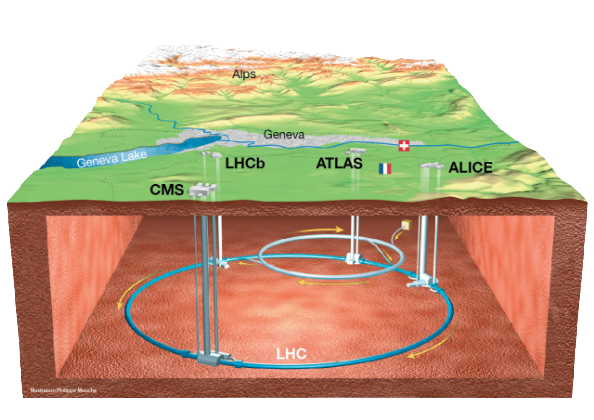
\includegraphics[width=1.1\textwidth]{Part2/Img/b_RTU_a_schematic_depiction_of_the_lhc-removebg-preview.png}
\end{figure}    
\end{columns}

\end{frame}

\subsection{The ATLAS detector}
\begin{frame}{The ATLAS detector}

\begin{columns}
\column{0.65\textwidth}
\begin{figure}
    \centering
    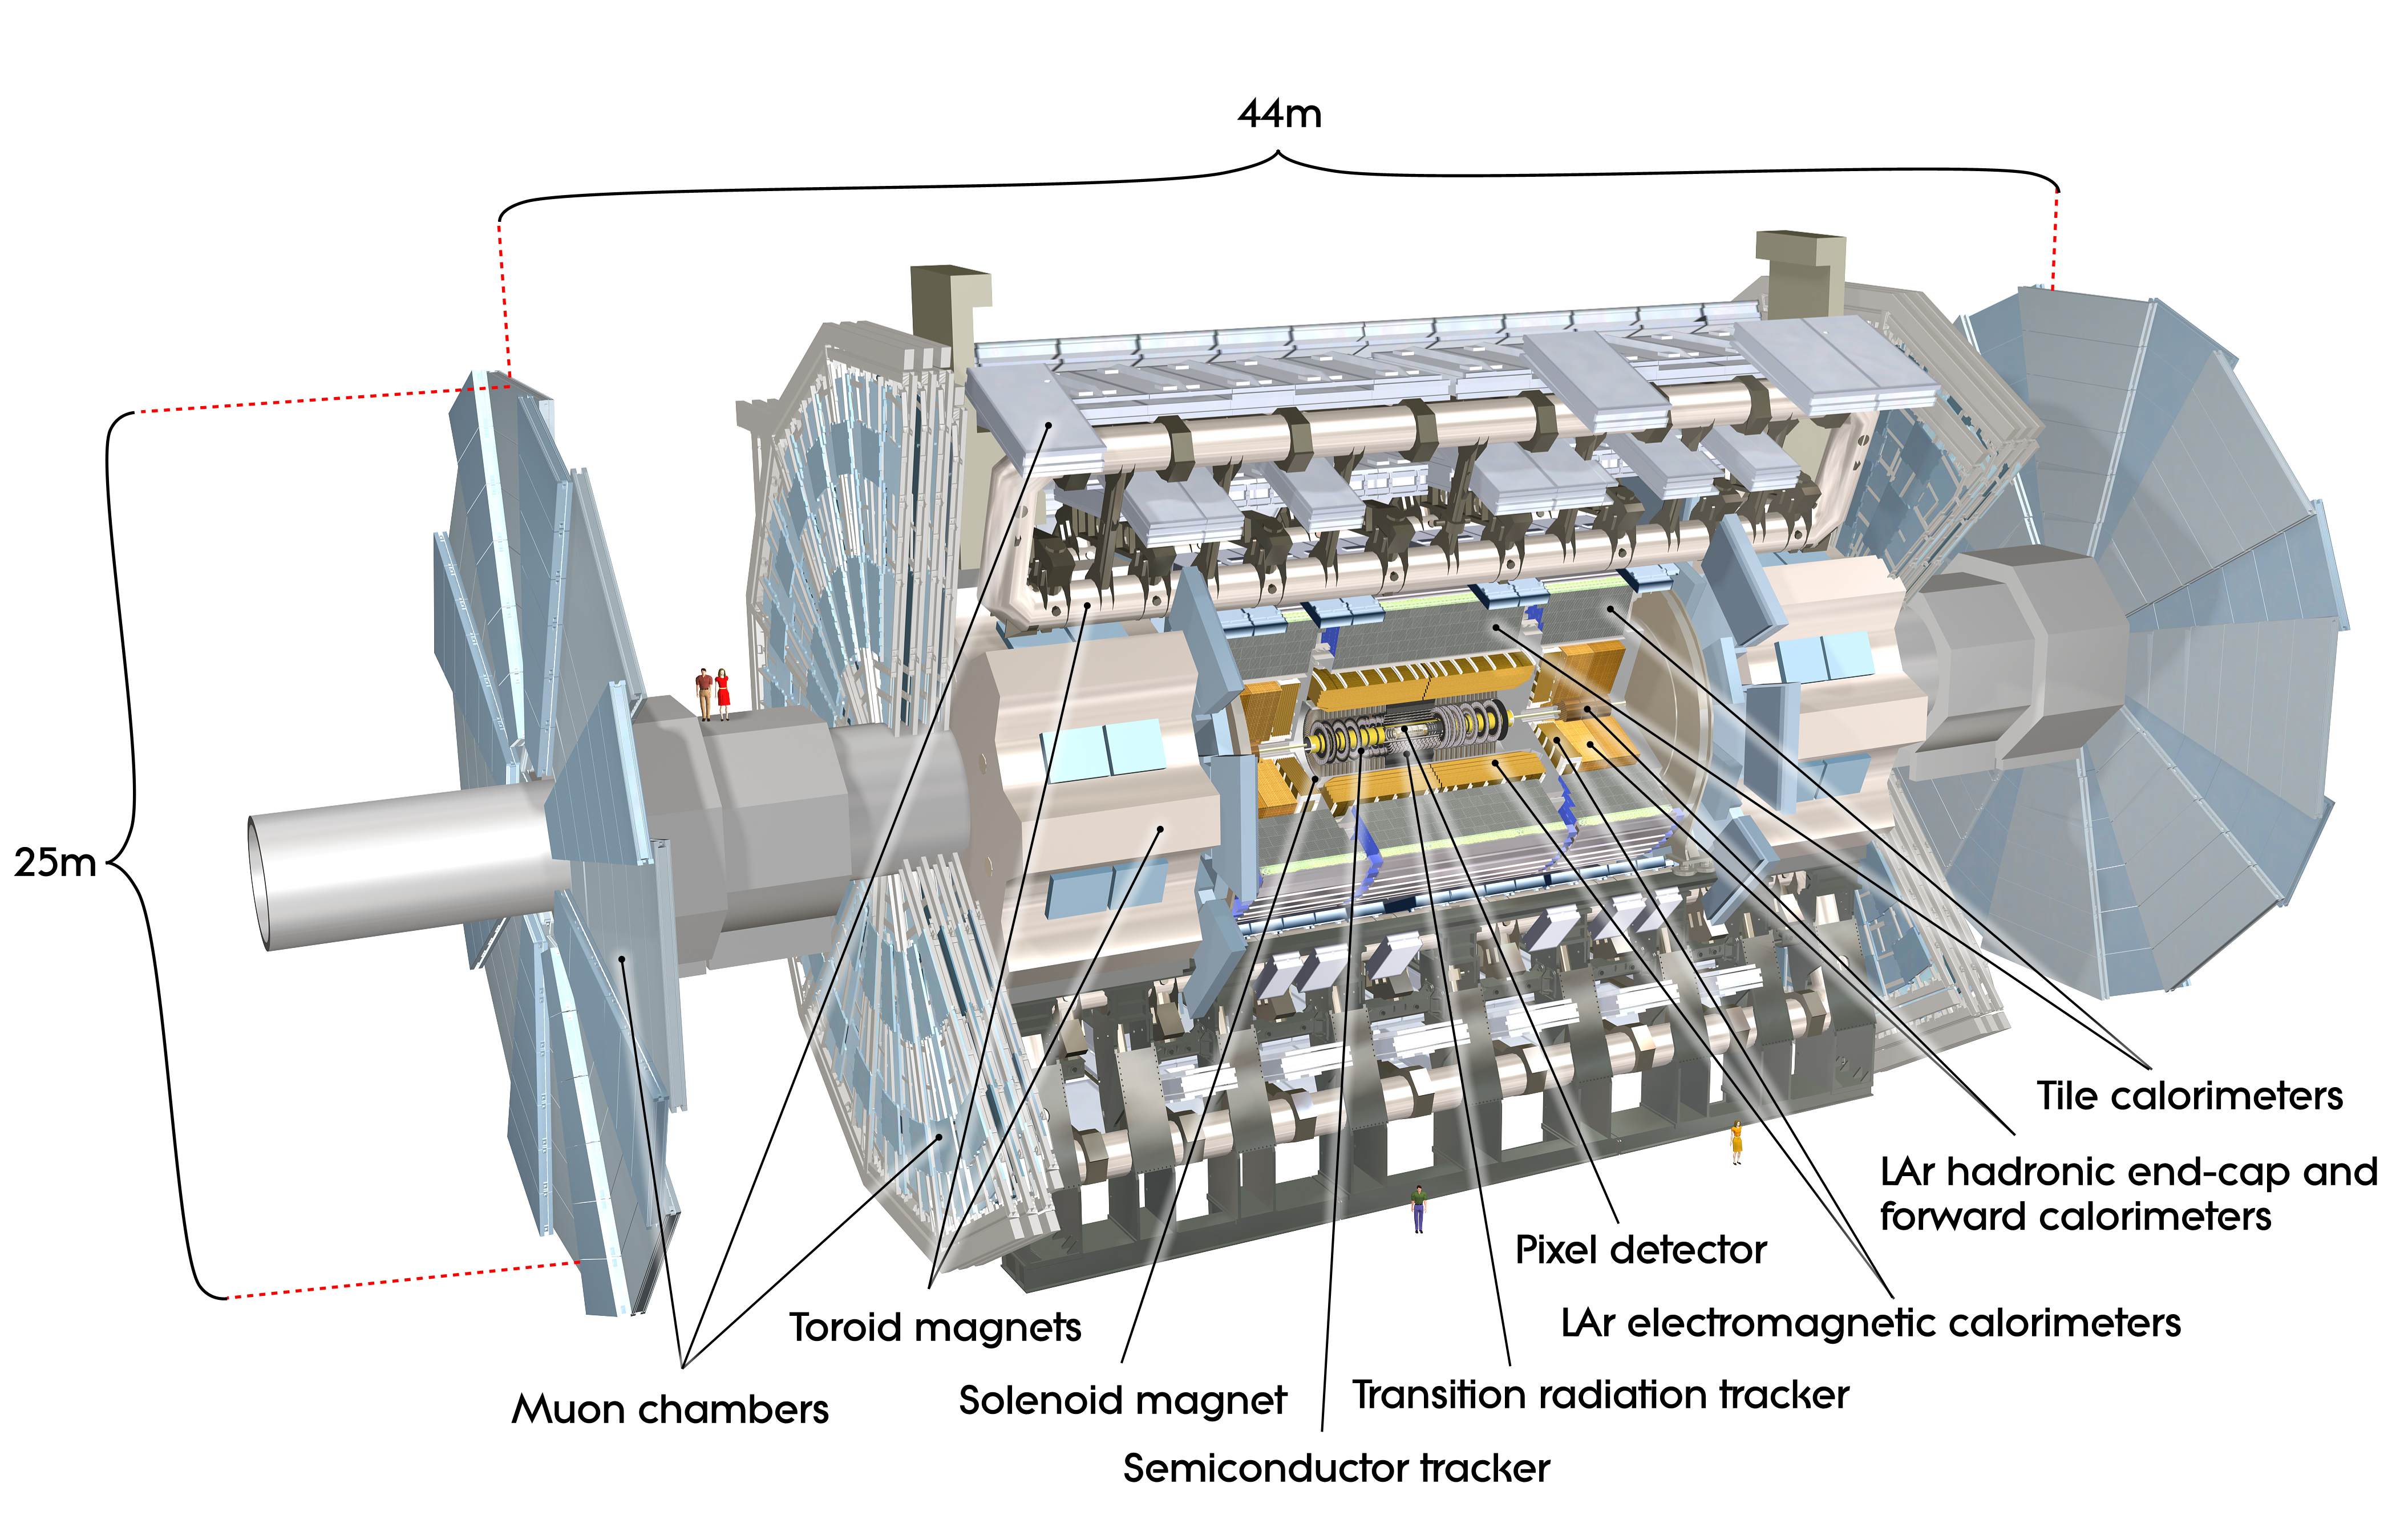
\includegraphics[width=1.\textwidth]{Part2/Img/ATLAS_sketch.jpg}
\end{figure}

\column{0.35\textwidth}

\begin{itemize}
    \item \textbf{Different sub-detectors}
    \item \textbf{Cylindrical} coordinate system
\end{itemize}
\begin{figure}
    \centering
    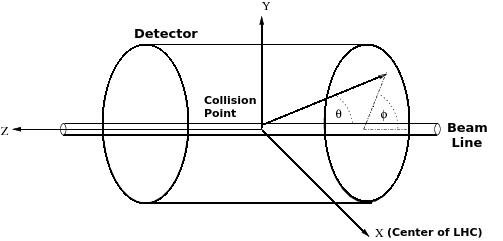
\includegraphics[width=1.\textwidth]{Part2/Img/ATLAS_Sys.jpeg}
\end{figure}
\begin{equation*}
    (p_T, \phi, \eta)
\end{equation*}
\begin{equation*}
    \textcolor{HHblue}{\eta = -\ln[\tan\frac{\theta}{2}]}
\end{equation*}
\end{columns}

\end{frame}

%\subsection{Particles reconstruction}
%\begin{frame}{Particles reconstruction}

%\begin{columns}
%\column{0.4\textwidth}

%\begin{itemize}
%    \item \textcolor{HHred}{Electrons} \& \textcolor{HHred}{Photons}
%    \begin{itemize}
%        \item EM cluster (+ ID track)
%    \end{itemize}
%    \item \textcolor{cadmiumorange}{Muons}
%    \begin{itemize}
%        \item Tracks
%    \end{itemize}
%    \item \textcolor{applegreen}{Hadrons} (jets)
%    \begin{itemize}
%        \item EM/Had clusters (+ ID track)
%    \end{itemize}
%    \item \textcolor{HHturquoise_l}{Neutrinos}
%    \begin{itemize}
%        \item Missing momentum
%    \end{itemize}
%\end{itemize}
%\column{0.6\textwidth}
%\begin{figure}
%    \centering
%    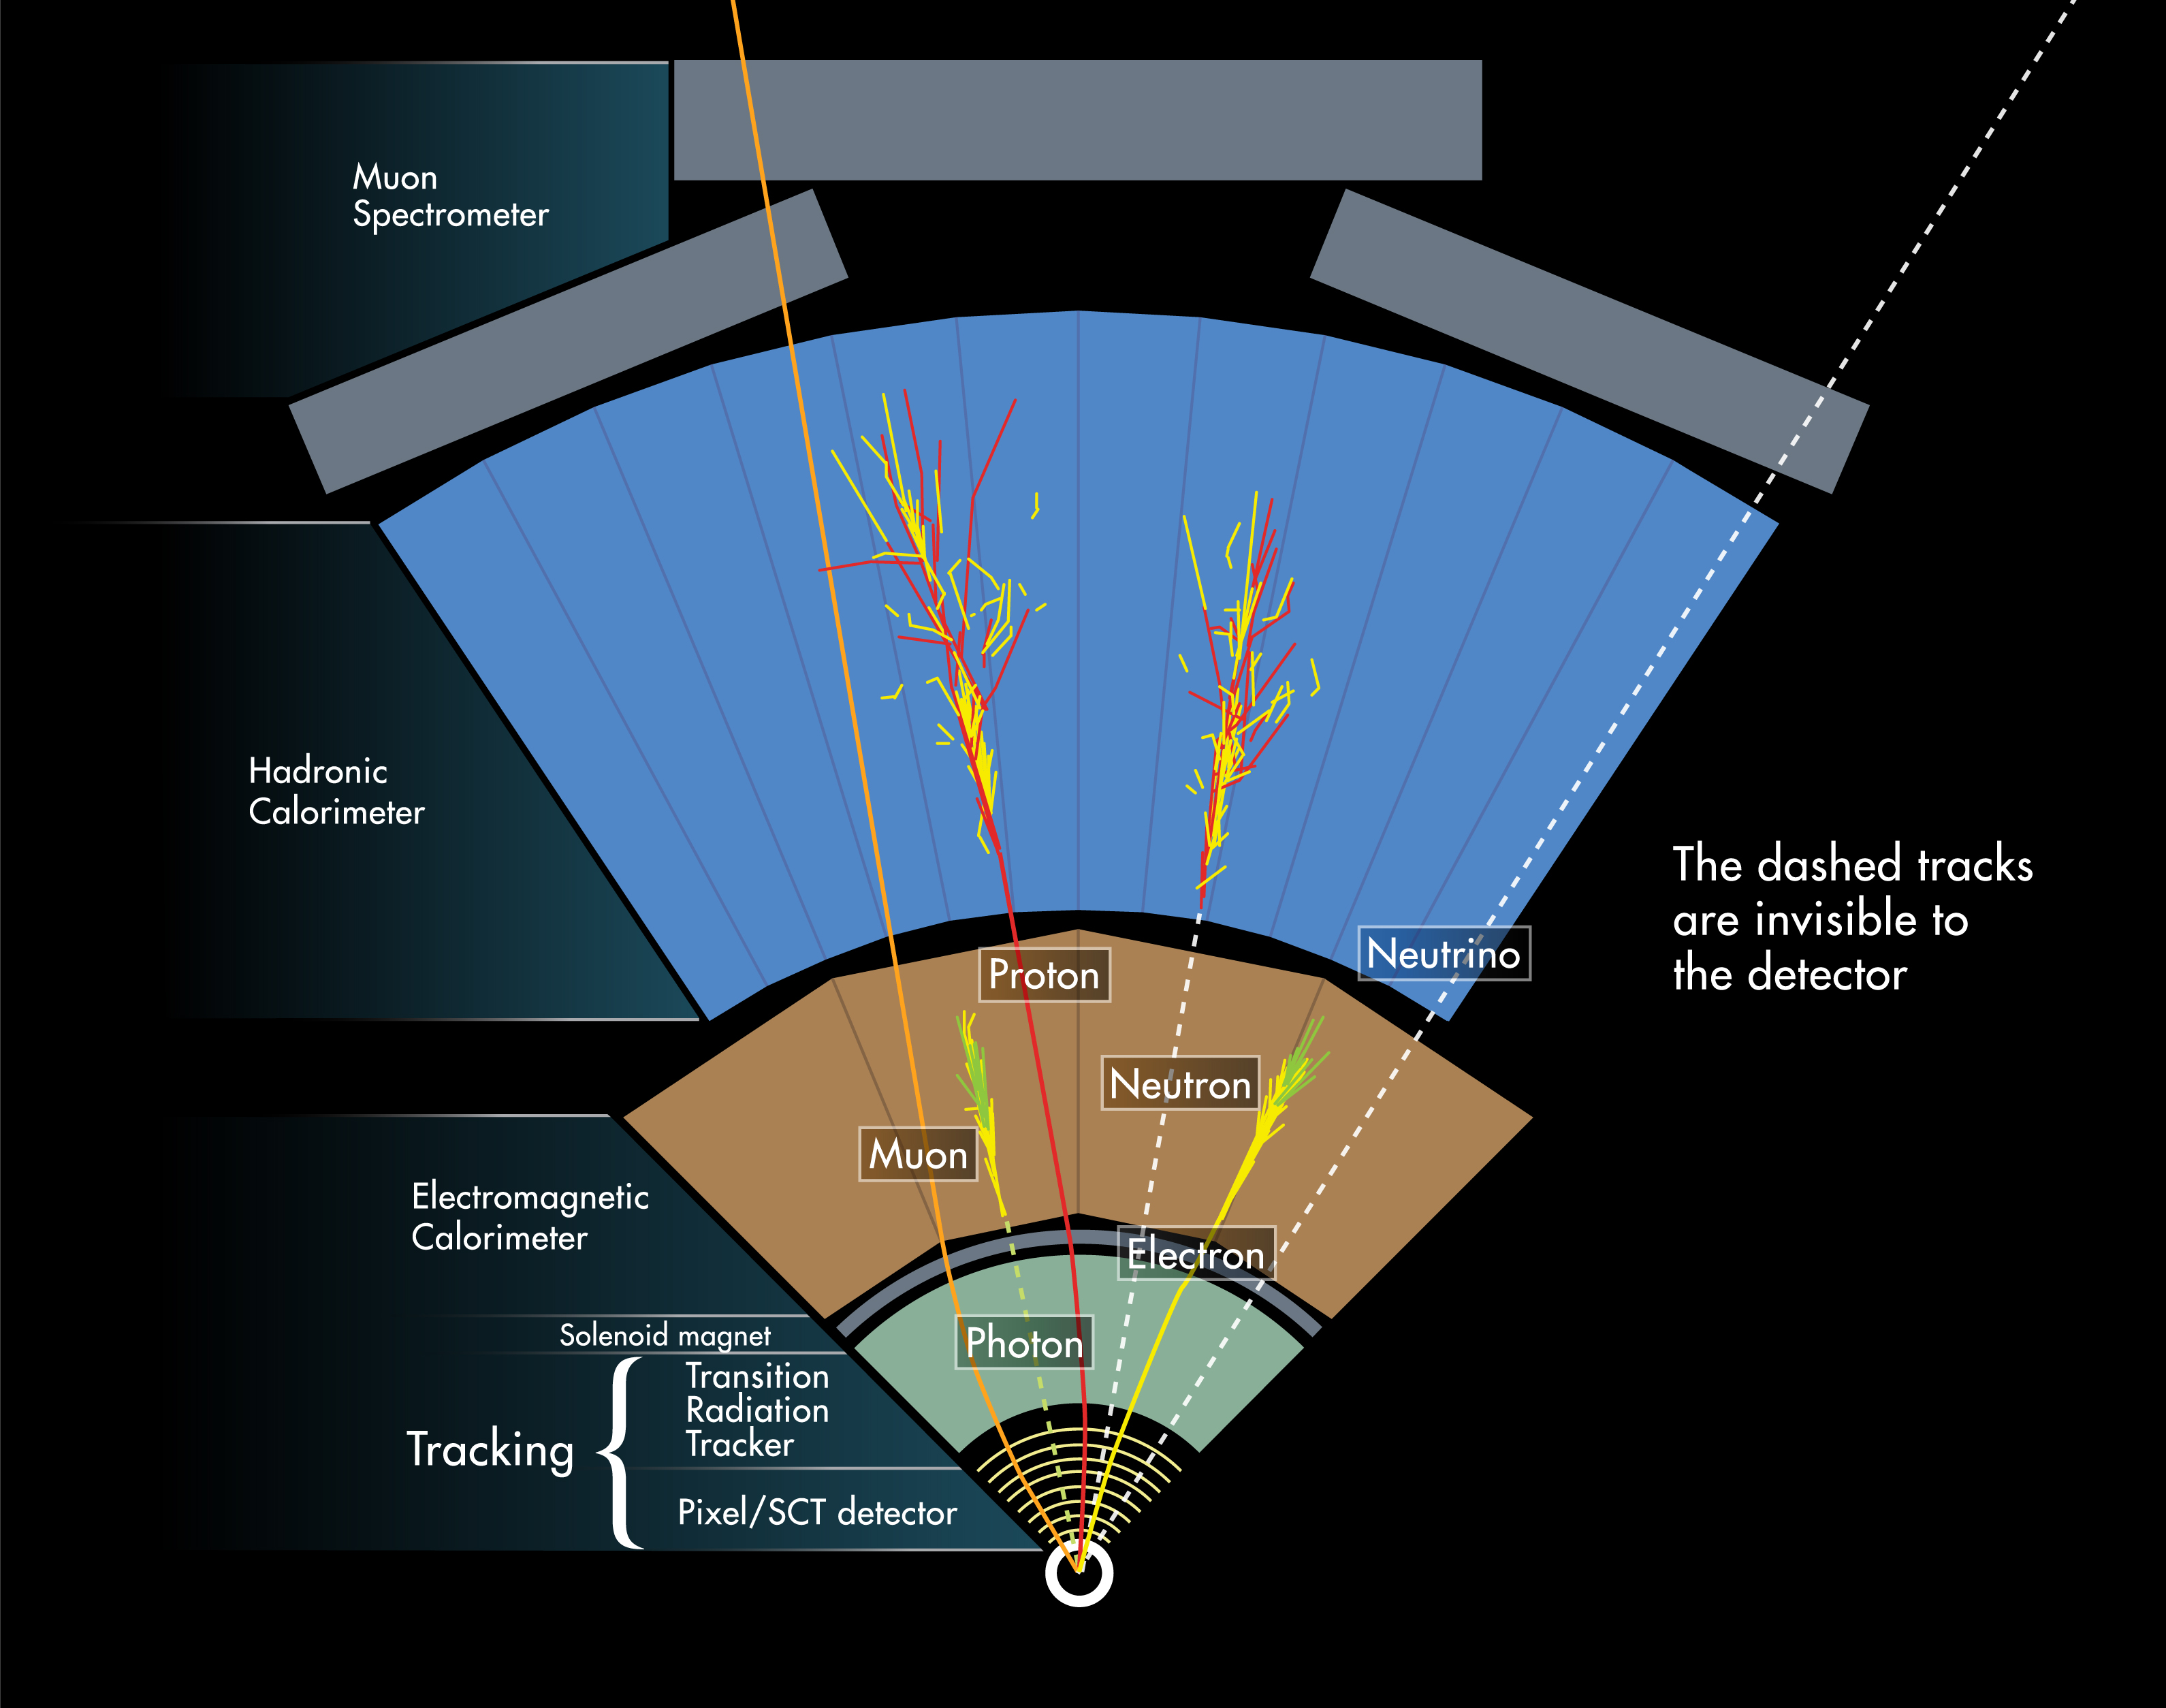
\includegraphics[width=1.\textwidth]{Part2/Img/Particle_detection.jpg}
   
%\end{figure}

%\end{columns}

%\end{frame}
\begin{frame}{Run-2 data taking}
    
\begin{textblock*}{5cm}(14.1cm, 3.2cm) % {block width} (coords) 
   \rotatebox{90}{\textbf{\textcolor{HHred}{--------------------------}}}
\end{textblock*}
\begin{textblock*}{5cm}(13.8cm, 4.1cm) % {block width} (coords) 
   \rotatebox{90}{\textbf{\textcolor{HHred}{Thesis begins}}}
\end{textblock*}
\begin{columns}
\column{0.5\textwidth}
\begin{itemize}
    \item Run-2 period: 2015-2018
    \item Integrated luminosity used for presented analysis: \textbf{139 fb$^{-1}$}
\end{itemize}


%\textcolor{HHblue}{\underline{Pile-up}}:
%\begin{itemize}
%    \item Dense environments 
%    \item \textbf{challenge!}
%\end{itemize}

%\begin{figure}
%    \centering
%     \fcolorbox{HHblue}{HHwhite2}{
%    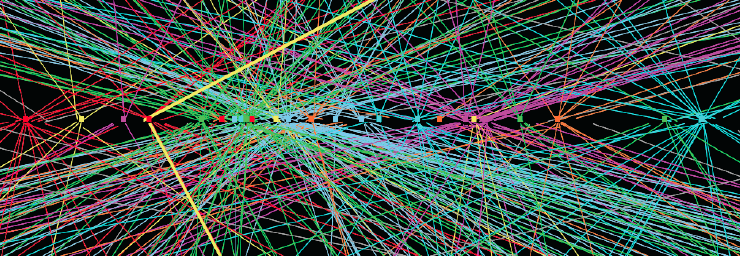
\includegraphics[width=0.8\textwidth]{Part2/Img/PileupEvent.png}
%    }
%\end{figure}
\column{0.5\textwidth}

\begin{textblock*}{5cm}(10cm, 5.4cm) % {block width} (coords) 
  \textcolor{black}{2015-2016 \\ (36 fb$^{-1}$)}
\end{textblock*}

\begin{figure}
    \centering
     \fcolorbox{HHred}{HHwhite2}{
    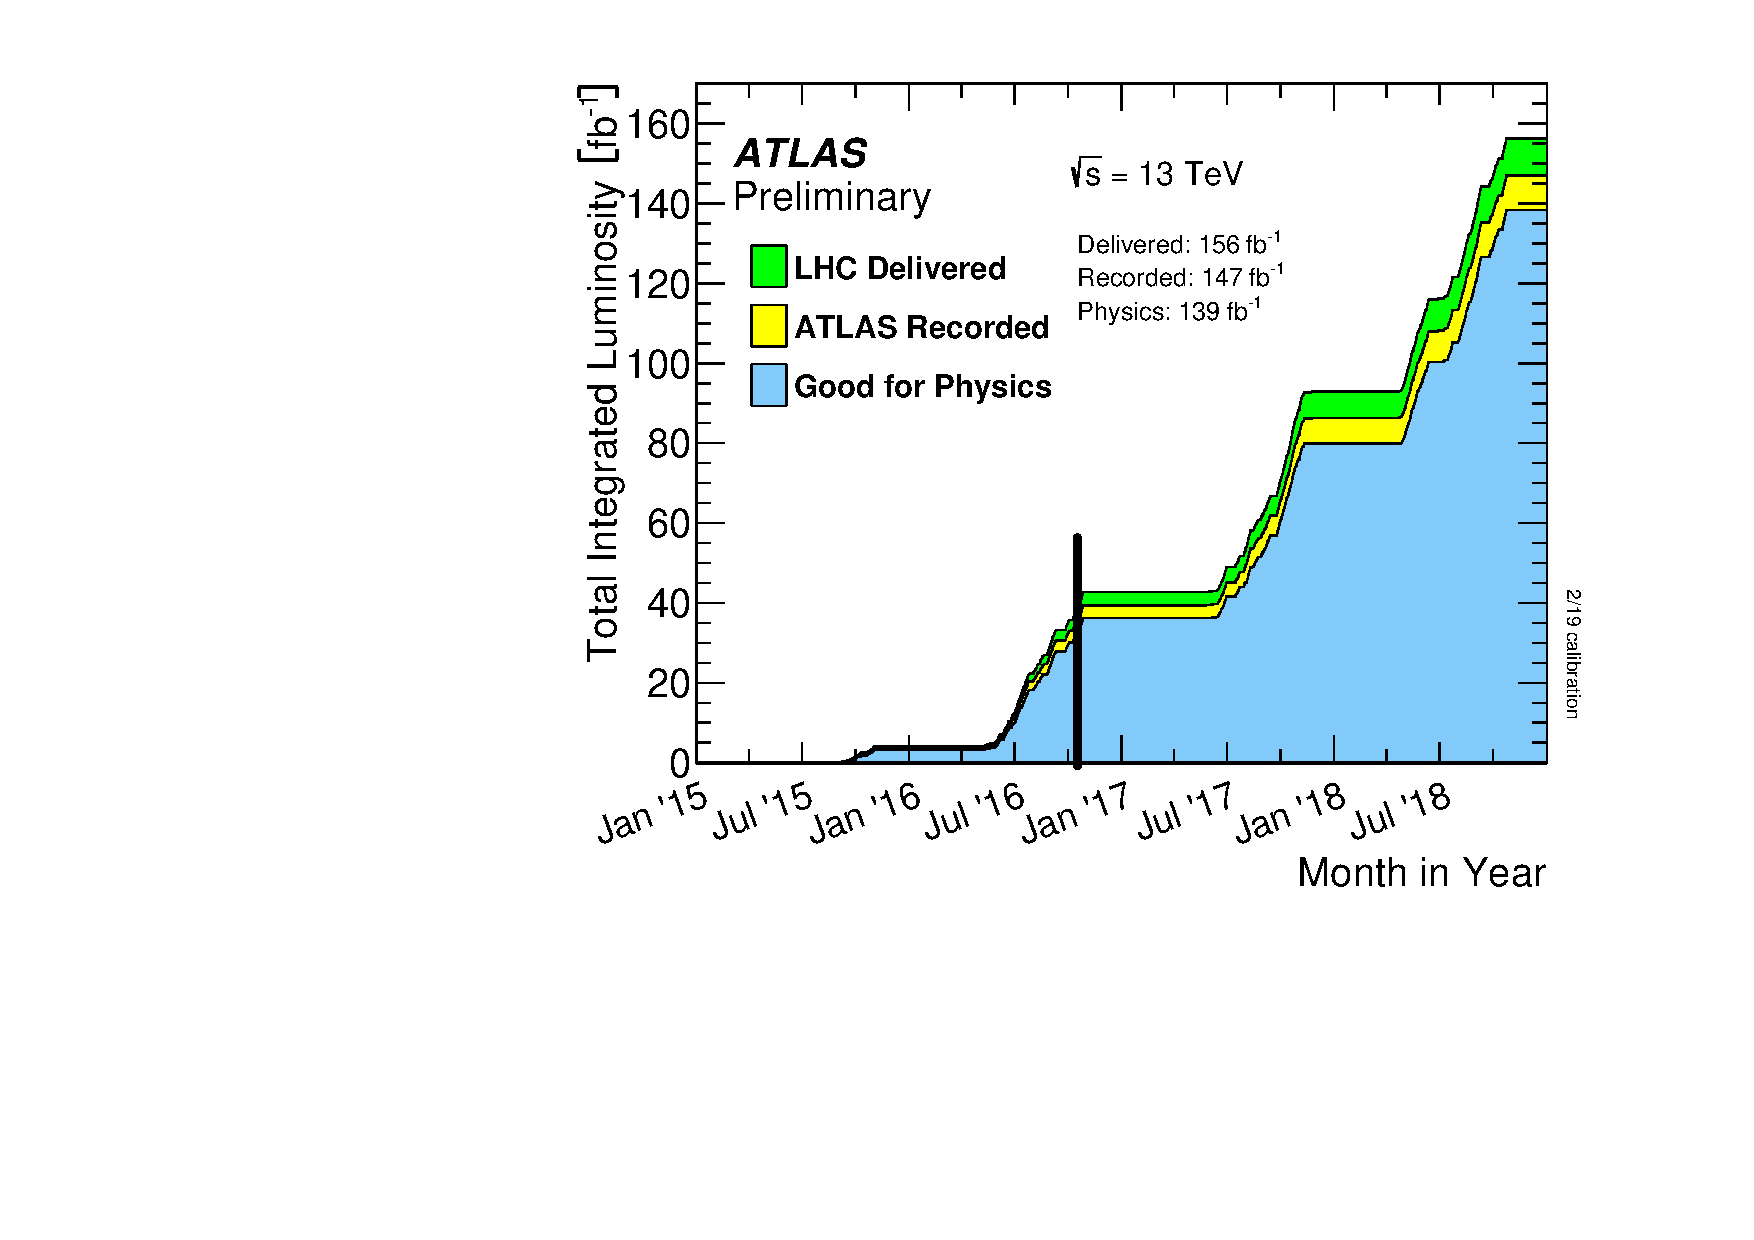
\includegraphics[width=1.\textwidth]{Part2/Img/intlumivstimeRun2DQall_edit.pdf}
    }
\end{figure}

%\begin{figure}
%    \centering
%     \fcolorbox{HHblue}{HHwhite2}{
%    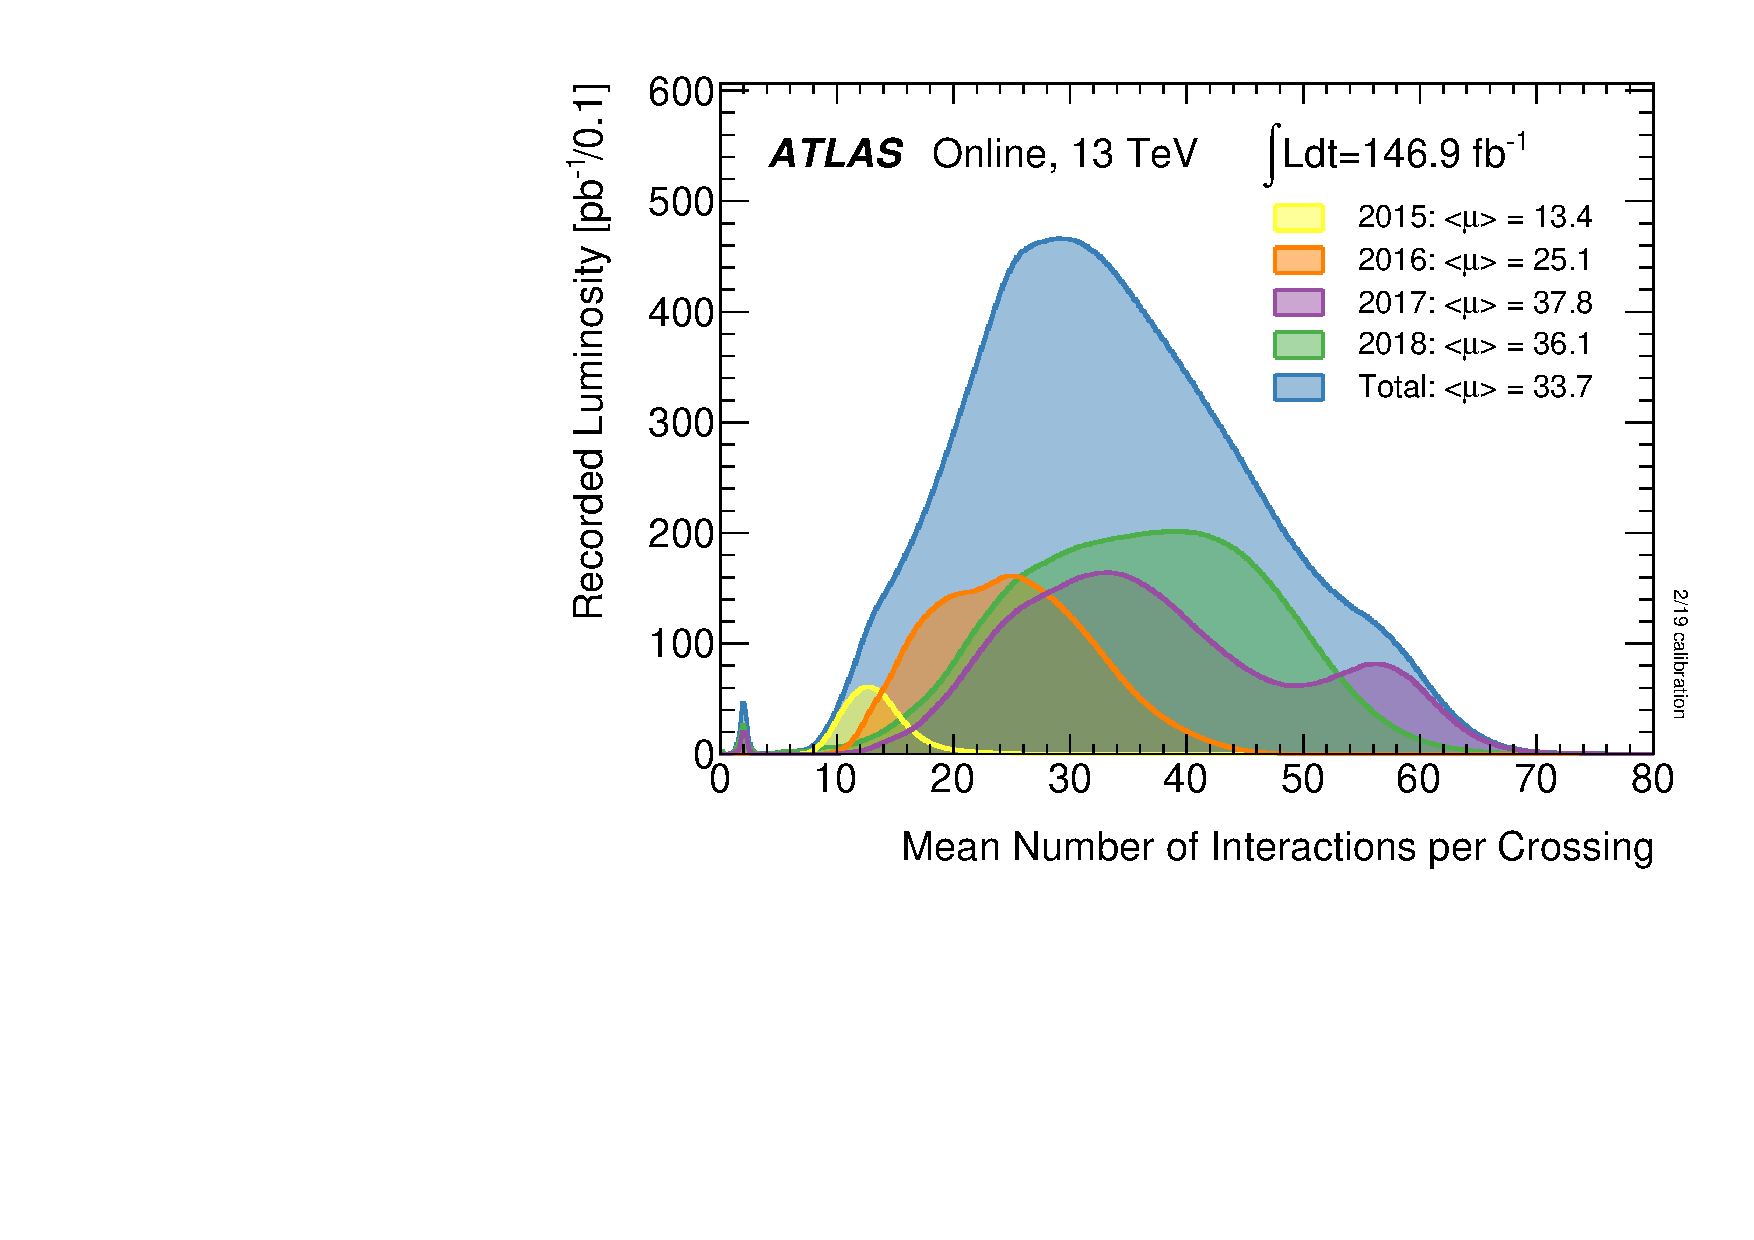
\includegraphics[width=0.55\textwidth]{Part2/Img/mu_2015_2018.pdf}
%    }
%\end{figure}

\end{columns}  
\end{frame}

\begin{frame}{Where are we with HH$\to b\bar{b}\gamma\gamma$?}
 
\begin{textblock*}{5cm}(8.5cm,2.8cm) % {block width} (coords) 
   \textcolor{applegreen}{\textbf{\href{https://link.springer.com/article/10.1007\%2FJHEP11\%282018\%29040}{JHEP 11 (2018) 040}}}
\end{textblock*}

\begin{itemize}
    \item Previous analysis: \textbf{\textcolor{applegreen}{2015-2016 data (36 fb$^{-1}$)}}
    \begin{itemize}
        \item $\frac{\sigma_{ggF}}{\sigma^{SM}}(HH)$ limit: \textbf{\textcolor{structurColor}{22}} (Exp. \textbf{28}) at 95\% CL
        \item $\kappa_{\lambda}$ constrain: \textbf{\textcolor{structurColor}{[-8.2, 13.2]}} (Exp. \textbf{[-8.3, 13.2]})
    \end{itemize}
\pause    
    \item My thesis: \textbf{\textcolor{HHred}{Full run-2 data (139 fb$^{-1}$)}}
    \begin{itemize}
        \item Improve the analysis sensitivity with different tools
    \end{itemize}
\end{itemize}    
\vspace{1em}
\begin{tabular}{lccc}
    \hline 
    \hline
     & HH & HH$\to b\bar{b}\gamma\gamma$ & $\sim$10\% eff. \\
     \hline
    Events  & 4.3k & 11 & $\mathcal{O}(1)$ \\
      \hline\hline 
\end{tabular}    
\end{frame}

\section{Measurement of Higgs self-coupling}

\begin{frame}{Content}
\label{content}
    \begin{columns}[t]
        \begin{column}{.5\textwidth}
            \tableofcontents[sections={1-5},currentsection]
        \end{column}
        \begin{column}{.5\textwidth}
            \tableofcontents[sections={6-},currentsection]
        \end{column}
    \end{columns}
\end{frame}

{
\usebackgroundtemplate{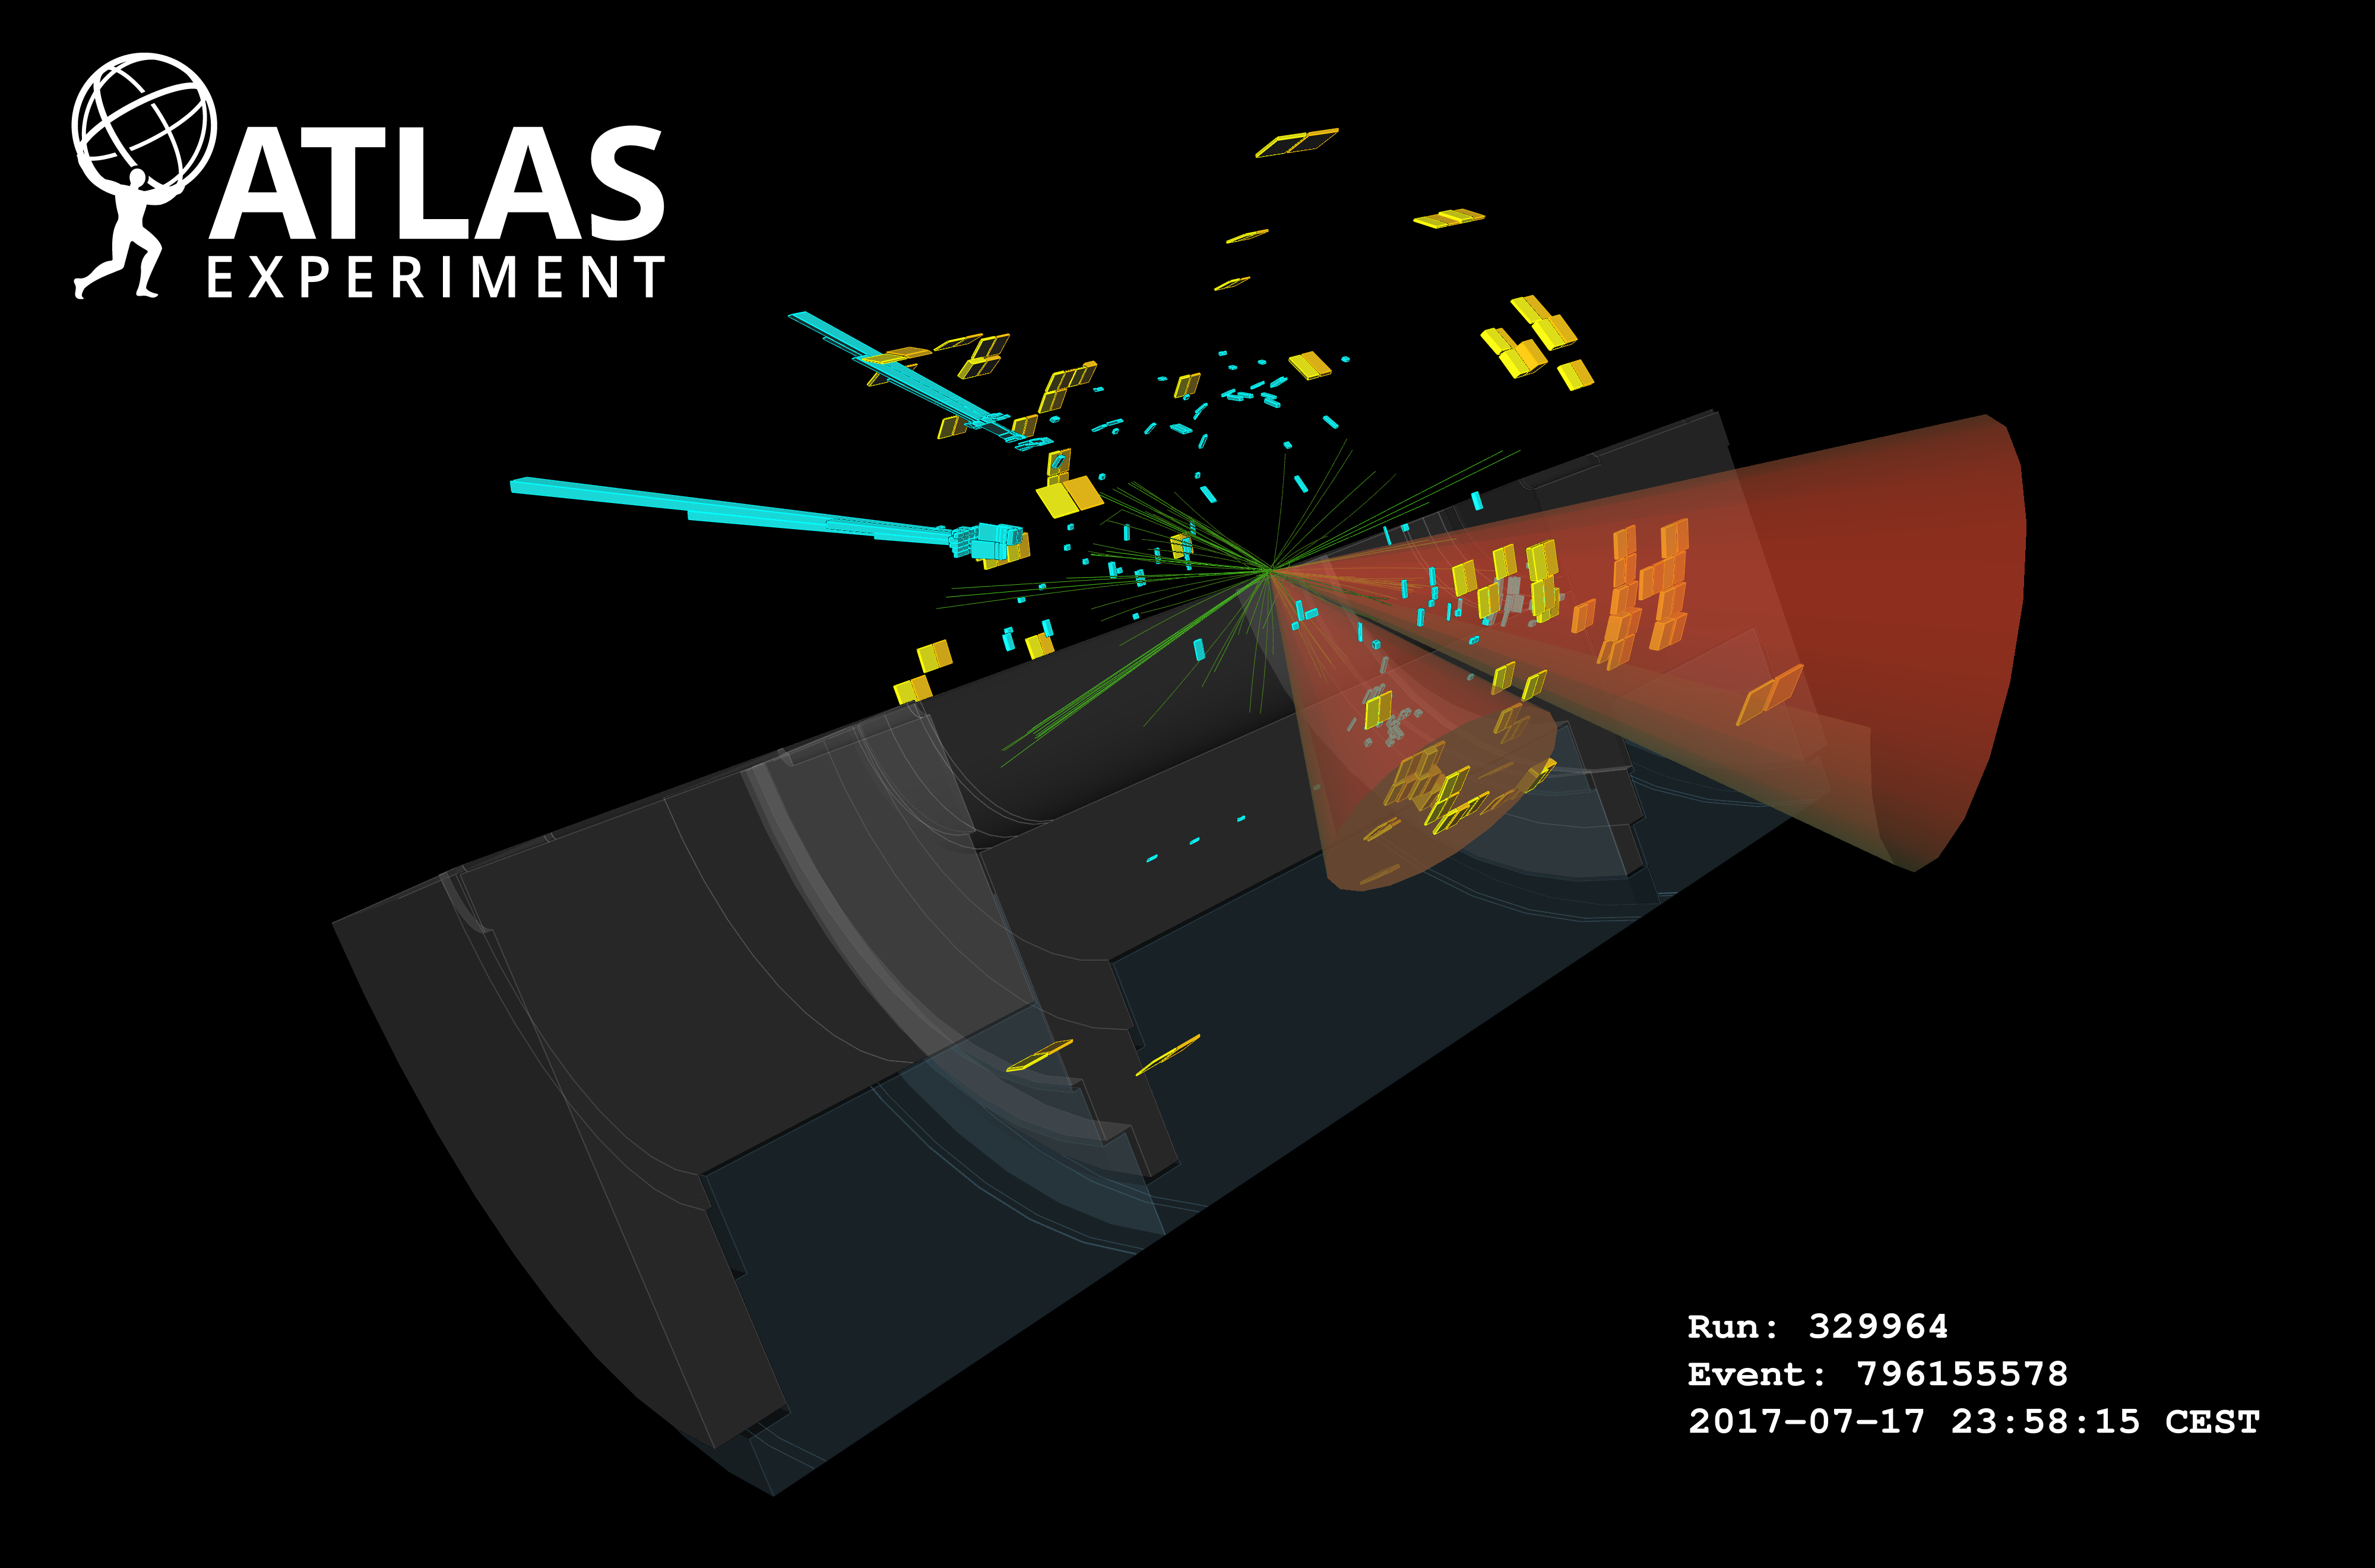
\includegraphics[width=1.03\paperwidth]{Img/figaux_01}}
\begin{frame}

\begin{textblock*}{6cm}(0.5cm,3.8cm) % {block width} (coords) 
   \textcolor{HHwhite2}{\textbf{Two narrow EM clusters $\to$ photons}}
\end{textblock*}

\begin{textblock*}{6cm}(10cm,7cm) % {block width} (coords) 
   \textcolor{HHwhite2}{\textbf{Two displaced vertices $\to$ $b$-jets}}
\end{textblock*}

\begin{textblock*}{7cm}(1cm,7cm)
 \visible<2>{% {block width} (coords) 
   \textcolor{HHwhite2}{\underline{\textbf{Backgrounds}}} \\
   \begin{itemize}
       \item \textcolor{HHwhite2}{Peaking in $m_{\gamma\gamma}$: \textbf{single H$\to\gamma\gamma$} ($t\bar{t}$H, ZH)}
       \item \textcolor{HHwhite2}{Not peaking:  \textbf{continuum $\gamma\gamma$ + jets}} 
   \end{itemize}
   }
\end{textblock*}


\end{frame}
}

\subsection{Analysis strategy}
\begin{frame}{Events selection}
\begin{columns}
\column{0.6\textwidth}

\begin{itemize}
    \item \textbf{Di-photon trigger} (83\% efficiency for HH signal)
    \begin{itemize}
        \item $E_{T}^{\gamma} > $ 35 (25) GeV for leading (sub-leading)
    \end{itemize}
    \item \textbf{$\geq $ 2 Tight} and \textbf{isolated} \textbf{photons} (\textbf{\textcolor{HHturquoise_d}{H$\to\gamma\gamma$}})
    \begin{itemize}
        \item $|\eta|< $ 2.37 \& $\frac{p_{T}^{\gamma}}{m_{\gamma\gamma}} > $ 35\% (25\%) for leading (sub-leading)
        \item $m_{\gamma\gamma}$ built with the two leading photons
    \end{itemize}
    \item \textbf{Exactly 2 $b$-jet} (\textbf{\textcolor{HHred}{H$\to b\bar{b}$}})
    \begin{itemize}
        \item $p_{T} > $ 25 GeV \& $|\eta| < $ 2.5
        \item $b$-tagging at 77\% efficiency
    \end{itemize}
    \item $<$ 6 jets, reject hadronic $t\bar{t}$H
    \item Zero leptons, reject semi-leptonic $t\bar{t}$H
\end{itemize}

\column{0.4\textwidth}

\begin{figure}
    \centering
    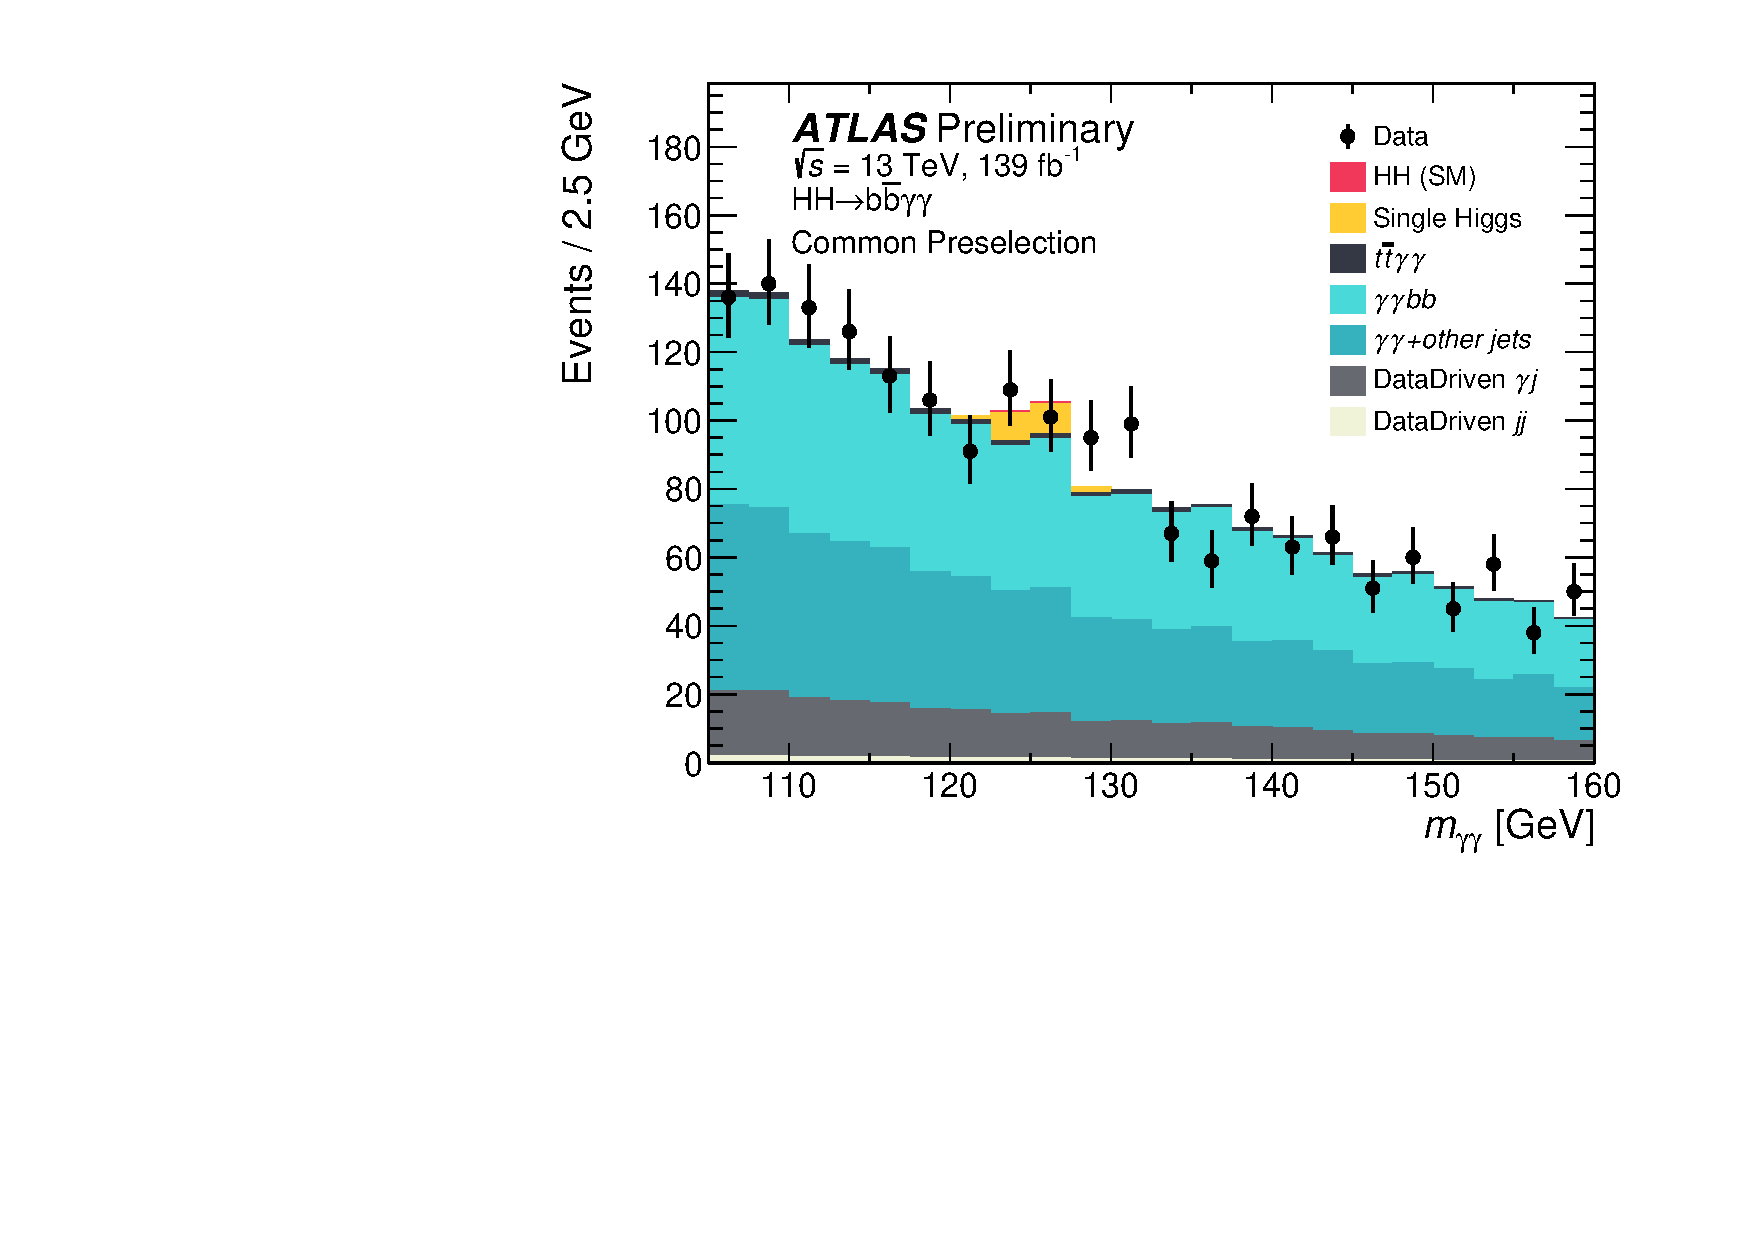
\includegraphics[width=1.1\textwidth]{Part3/Img/myy_common.pdf}
\end{figure}
\begin{center}
%\textbf{Dominant backgrounds}
%\begin{itemize}
%    \item \textbf{\textcolor{HHyellow}{Single H}} (peaking in $m_{\gamma\gamma}$): \\ \textbf{$t\bar{t}$H} + \textbf{ZH} 
%    \item \textcolor{HHturquoise_m}{\textbf{Continuum $\gamma\gamma$ + jets}}
%\end{itemize}

\end{center}
%\begin{figure}
%    \centering
%    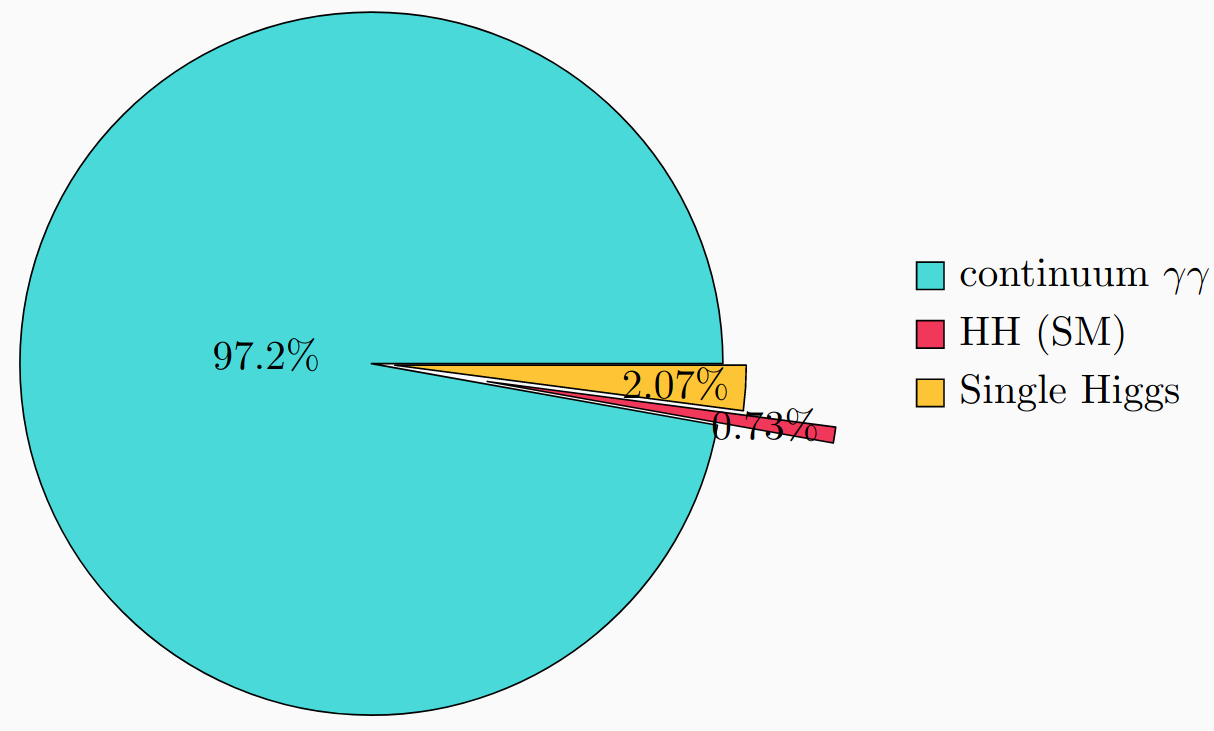
\includegraphics[width=0.7\textwidth]{Part3/Img/pie.png}
%\end{figure}

\end{columns}

\end{frame}

\begin{frame}{$b$-jet energy calibration}

\begin{textblock*}{5cm}(12cm,0.1cm) % {block width} (coords) 
   \textcolor{HHred}{\Large\textbf{my own work}}
\end{textblock*}

\begin{columns}
\column{0.4\textwidth}
\begin{figure}
    \centering
    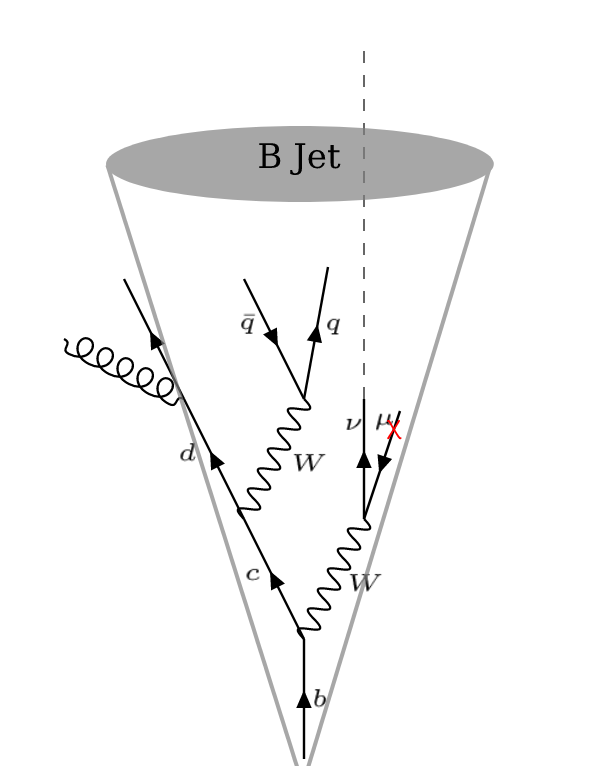
\includegraphics[width=0.8\textwidth]{Part3/Img/b-jet.png}
\end{figure}

\column{0.6\textwidth}

\begin{itemize}
    \item $m_{b\bar{b}}$ highly discriminating for H$\to b\bar{b}$
    \item $\sigma_{m_{b\bar{b}}}\sim$ 16 GeV, $\sigma_{m_{\gamma\gamma}}\sim$ 2 GeV
    \item Jets energy calibration not enough for $b$-jets,\\ due to 
    \begin{itemize}
        \item \textcolor{HHred}{\textbf{Semi-leptonic}} decay
        \item \textcolor{HHturquoise_d}{\textbf{Large $b$-quark mass}}
    \end{itemize}
\pause    
    \item Specific $b$-jet energy calibration method
    \begin{itemize}
        \item \textcolor{HHred}{\textbf{$\mu$-in-jet correction}}: presence of \textbf{muon} 
        \item \textcolor{HHturquoise_d}{\textbf{$p_T$Reco correction}}: \textbf{missing neutrino} \& \textbf{out-of-cone} radiation
    \end{itemize}
\end{itemize}
\end{columns}
\end{frame}

\begin{frame}{$b$-jet energy calibration}
\begin{textblock*}{5cm}(12cm,0.1cm) % {block width} (coords) 
   \textcolor{HHred}{\Large\textbf{my own work}}
\end{textblock*}
\begin{textblock*}{5cm}(1.9cm, 7.48cm) 
--------------------------------------
\end{textblock*}
\begin{columns}
\column{0.5\textwidth}
\begin{itemize}
    \item \textcolor{HHred}{\textbf{$\mu$-in-jet} correction}
    \begin{itemize}
        \item Adding back muons
        \item Variable $\Delta R$($b$-jet, muon) 
        \item Semi-leptonic or hadronic
    \end{itemize}
    \item \textcolor{HHturquoise_d}{\textbf{$p_T$Reco} correction}
    \begin{itemize}
        \item $p_T$-dependent scale factor
        \item Computed on \textbf{$t\bar{t}$ sample}
    \end{itemize}
\end{itemize}
\begin{figure}
    \centering
    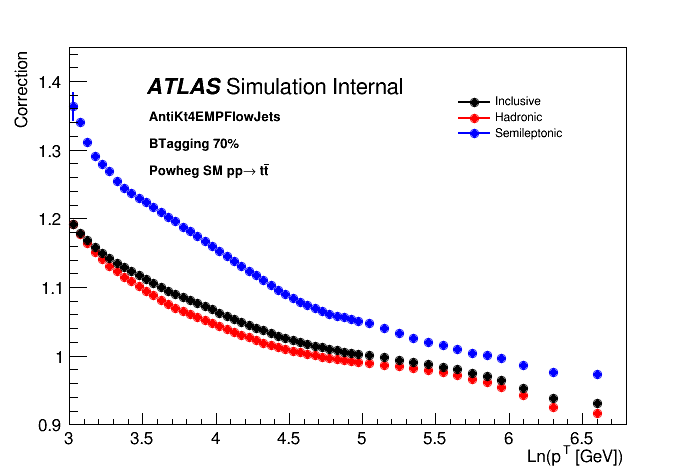
\includegraphics[width=0.8\textwidth]{Part3/Img/ptrecopflow.png}
\end{figure}

\column{0.5\textwidth}
\visible<2->{
\begin{itemize}
    \item Applied to HH$\to b\bar{b}\gamma\gamma$ $b$-jets
\end{itemize}
}
\visible<2->{
\begin{figure}
    \centering
    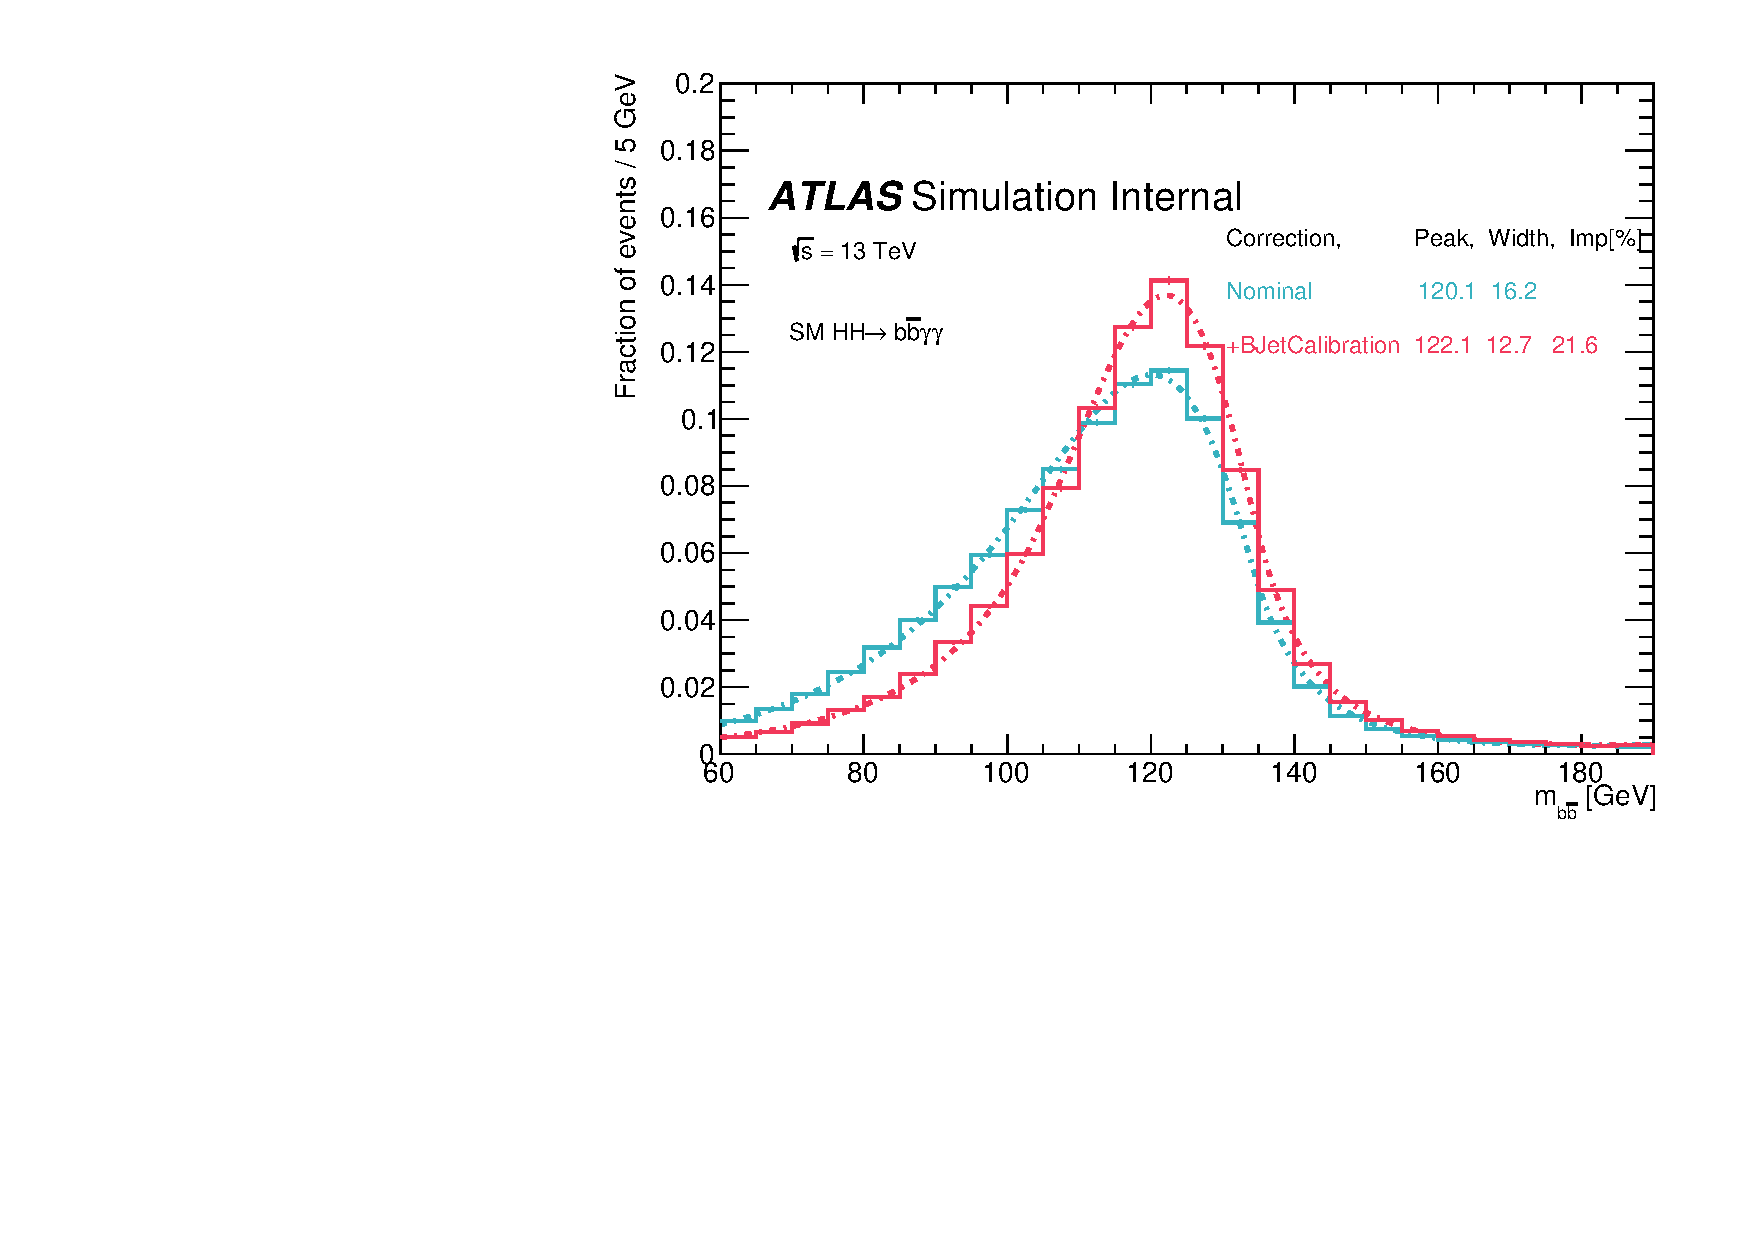
\includegraphics[width=0.9\textwidth]{Part3/Img/mbb_Paper.pdf}
\end{figure}

\begin{itemize}
    \item \textcolor{HHred}{\textbf{$\sim$22\%}} imp. on $m_{b \bar{b}}$ resolution
    \item \textcolor{HHred}{\textbf{7\% $\pm$ 2\%}} imp. on expected significance
    \item \textsl{\textbf{Baseline $b$-jet correction} for full Run-2 HH search}
\end{itemize}
}
\end{columns}    
\end{frame}


\begin{frame}{Categorization strategy}

\begin{columns}
\column{0.5\textwidth}
\begin{itemize}
    \item Sensitivity to
    \begin{itemize}
        \item \textbf{\textcolor{HHred}{SM HH signal}}
        \item \textbf{\textcolor{HHturquoise_d}{
$\kappa_{\lambda}$ deviations}}
    \end{itemize}
\pause    
    \item Two mass regions on $m_{b \bar{b}\gamma\gamma}^{*}$
    \begin{itemize}
        \item \textbf{\textcolor{HHred}{High mass} $m_{b \bar{b}\gamma\gamma}^{*} >$ 350 GeV}
        \item \textbf{\textcolor{HHturquoise_d}{Low mass} $m_{b \bar{b}\gamma\gamma}^{*} <$ 350 GeV}
    \end{itemize}
\end{itemize}

\begin{itemize}
    \item Signal-background separation: \textbf{MVA}
\end{itemize}

\column{0.5\textwidth}

\begin{textblock*}{5cm}(11cm, 3.8cm) % {block width} (coords) 
   \visible<2->{\textbf{\textcolor{HHred}{High mass}}}
\end{textblock*}
\begin{textblock*}{5cm}(9.5cm, 2.8cm) % {block width} (coords) 
   \visible<2->{\textbf{\textcolor{HHturquoise_d}{Low mass}}}
\end{textblock*}
\begin{figure}
    \begin{overprint}
    \onslide<1>\centering\centering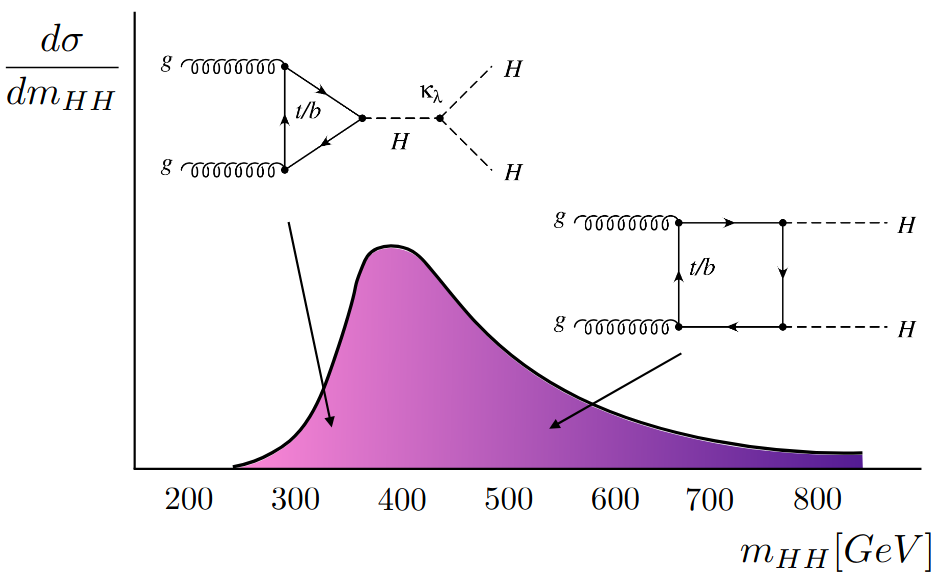
\includegraphics[width=1\textwidth]{Part3/Img/mHH_diagram2.png}
    \onslide<2->\centering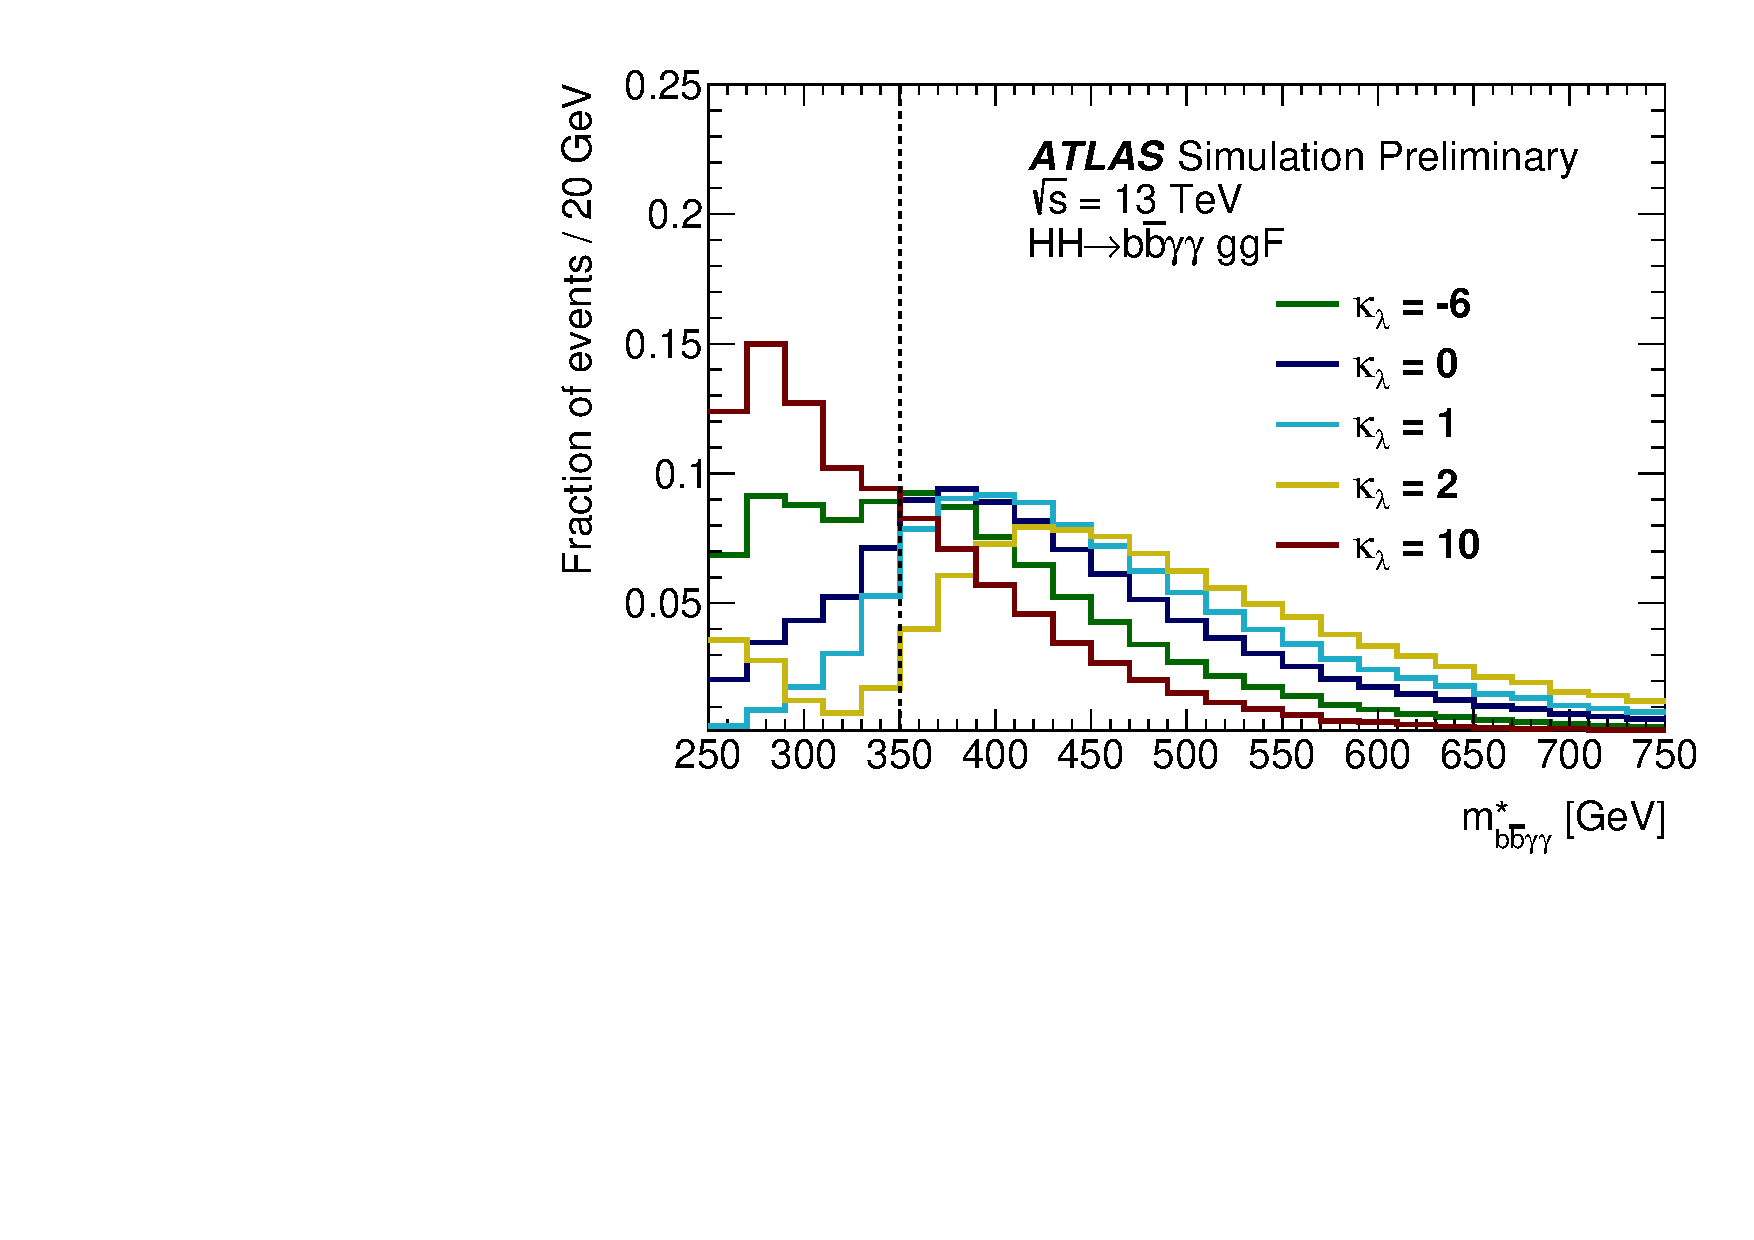
\includegraphics[width=1.1\textwidth]{Part3/Img/mbbyy_star_ggF.pdf}
    \end{overprint}
\end{figure}
\onslide<2->{
\begin{equation*}
    \textcolor{gray}{m_{b \bar{b}\gamma\gamma}^{*} =  m_{b \bar{b}\gamma\gamma} - m_{b \bar{b}} - m_{\gamma\gamma} + 250 \ \text{GeV}}
\end{equation*}
}
\end{columns}
\end{frame}

\begin{frame}{MVA categorization}

\begin{columns}
\column{0.6\textwidth}
\begin{itemize}
    \item Two MVA are trained to discriminate signal from the backgrounds
    \begin{itemize}
        \item \textbf{High mass}: \textbf{\textcolor{HHred}{SM HH ($\kappa_{\lambda} = $ 1)}}
        \item \textbf{Low mass}: \textbf{\textcolor{HHturquoise_d}{BSM HH ($\kappa_{\lambda} = $ 10)}}
    \end{itemize}
    \item Same inputs: objects and event kinematic
    \item MVA techniques
    \begin{itemize}
        \item \textcolor{structurColor}{\textbf{B}oosted \textbf{D}ecision \textbf{T}rees}: signal vs ($t\bar{t}$H + ZH + continuum $\gamma\gamma$ + jets)
        \item \textbf{D}eep \textbf{N}eural \textbf{N}etwork: signal vs $t\bar{t}$H vs ZH vs continuum $\gamma\gamma$ + jets
    \end{itemize}
\end{itemize}  

\column{0.4\textwidth}

\begin{figure}
    
    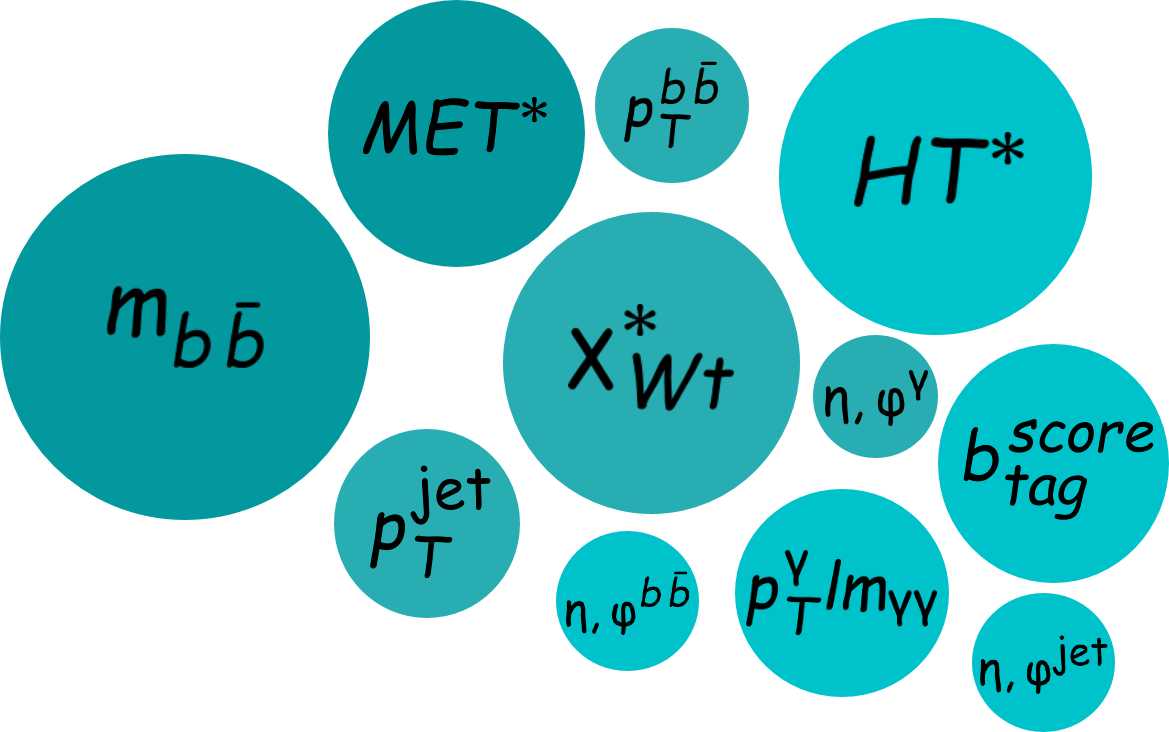
\includegraphics[width=1.\textwidth]{Part3/Img/MVA_vars.png}
\end{figure}
\textcolor{gray}{$^{*}$ not used in DNN} \\

%$\chi_{Wt}= \min \sqrt{\left(\frac{m_{j_{1} j_{2}}-m_{W}}{m_{W}}\right)^{2}+\left(\frac{m_{j_{1} j_{2} j_{3}}-m_{t}}{m_{t}}\right)^{2}}$

\end{columns}   
\end{frame}

\begin{frame}{Deep Neural Network selection}
\begin{textblock*}{5cm}(12cm,0.1cm) % {block width} (coords) 
   \textcolor{HHred}{\Large\textbf{my own work}}
\end{textblock*}
\begin{columns}
\column{0.4\textwidth}
\begin{itemize}
    \item $d_{HH}$ discriminate from 4 probabilities: 
    \begin{equation*}
        d_{HH} = \log(\frac{\sigma_{HH}.p_{HH}}{\sum^{3}{\sigma_{bkg}.p_{bkg}}})
    \end{equation*}
    \item \textbf{\textcolor{HHred}{4 categories}} maximize combined expected significance 
    \begin{itemize}
        \item \textbf{tight} and \textbf{loose} DNN for each mass region
    \end{itemize}
    \onslide<3->{
    \item \textbf{\textcolor{HHturquoise_d}{Similar performance to the BDT}}
    }
    \onslide<4->{
    \item Baseline: \textcolor{HHred}{\textbf{BDT}}
    \item \textsl{\textbf{DNN} reserved and documented for next analysis round}
    }
\end{itemize}

\column{0.6\textwidth}
\begin{textblock*}{5cm}(8.2cm, 2.4cm) % {block width} (coords) 
  \visible<1>{\rotatebox{90}{Event}}
\end{textblock*}

\begin{textblock*}{5cm}(8.5cm, 2.8cm)  
  \visible<1>{$\to$}
\end{textblock*}

\begin{textblock*}{5cm}(13.2cm, 2.3cm) 
 \visible<1>{\small \textcolor{HHturquoise_d}{HH signal}}
\end{textblock*}
\begin{textblock*}{5cm}(13.2cm, 2.6cm) % {block width} (coords) 
  \visible<1>{ \small \textcolor{HHblue}{$t\bar{t}$H}}
\end{textblock*}
\begin{textblock*}{5cm}(13.2cm, 2.9cm) % {block width} (coords) 
   \visible<1>{\small \textcolor{HHred}{ZH}}
\end{textblock*}
\begin{textblock*}{5cm}(13.2cm, 3.2cm) % {block width} (coords) 
   \visible<1>{\small \textcolor{cadmiumorange}{continuum $\gamma\gamma$+jets}}
\end{textblock*}
\begin{figure}
   \begin{overprint}
   \onslide<1>\centering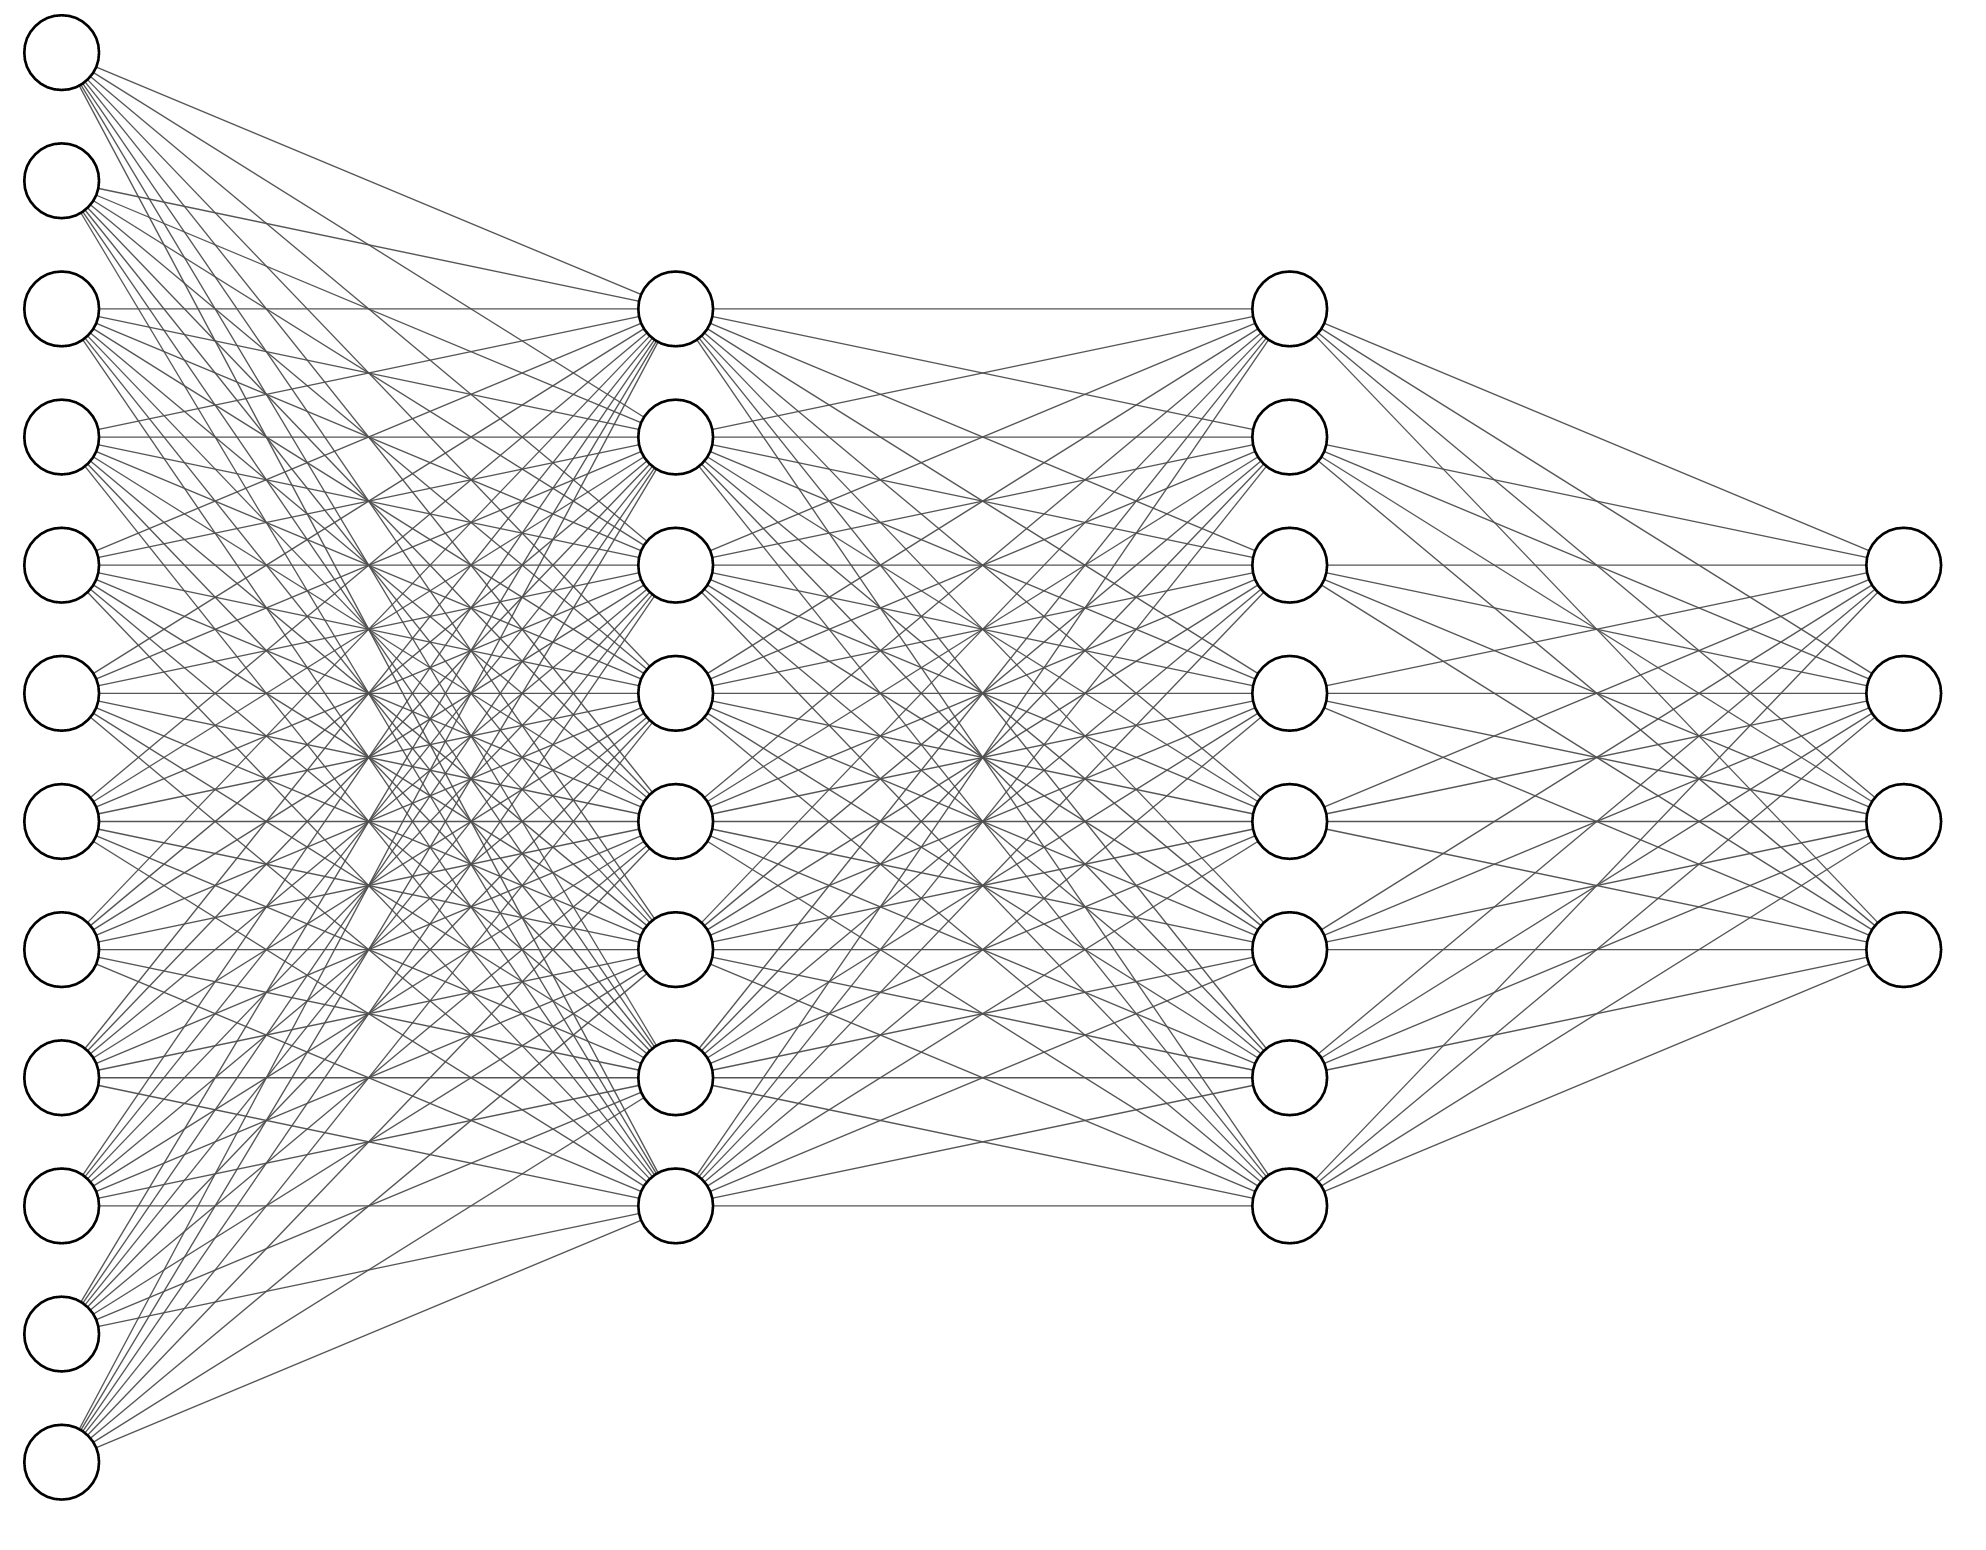
\includegraphics[width=0.5\textwidth]{Part3/Img/DNN.png}
   \onslide<2->\centering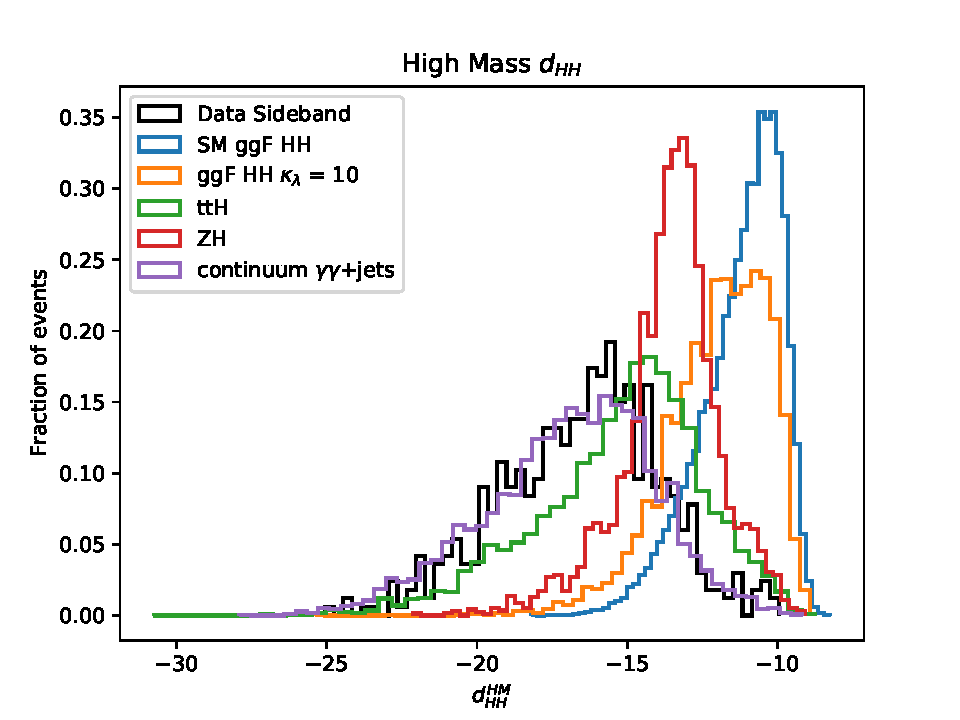
\includegraphics[width=0.7\textwidth]{Part3/Img/dHH_SM.pdf}
   \end{overprint}
 %   \subfloat{ 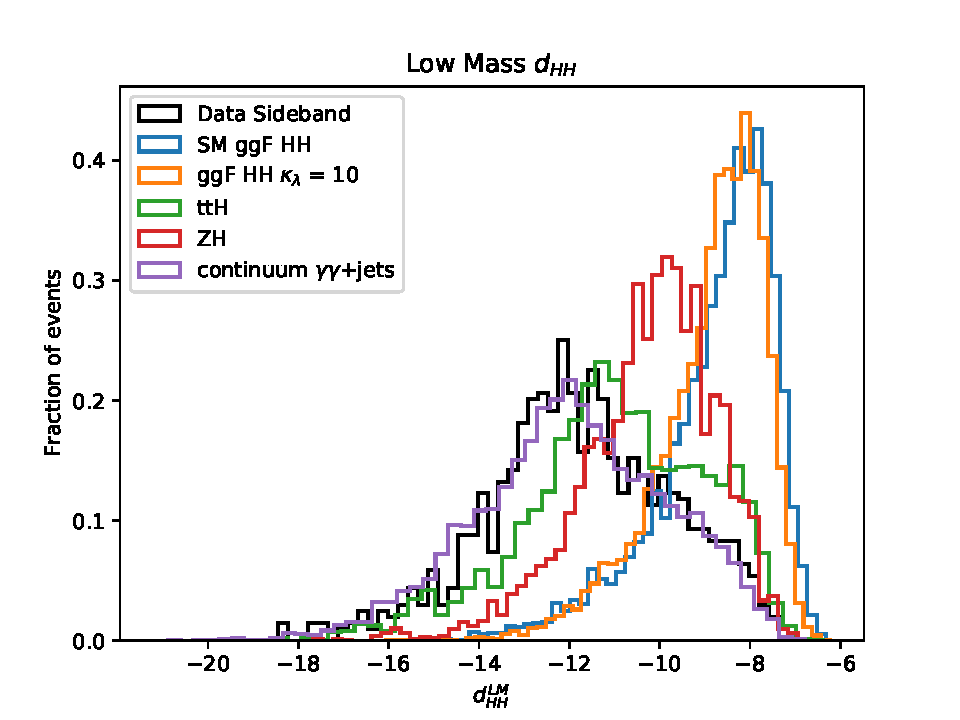
\includegraphics[width=0.55\textwidth]{Part3/Img/dHH_BSM.pdf}}
\end{figure}

\onslide<3->{
\begin{table}
    \centering
    \begin{tabular}{lcc}
    \hline\hline
        MVA & SM HH & HH $\kappa_{\lambda} = $ 10 \\
        \hline
        BDT & 0.49$\sigma$ & 3.59$\sigma$ \\
        DNN & 0.54$\sigma$ & 3.47$\sigma$ \\
        \hline\hline
    \end{tabular}
\end{table}
\begin{center}
  \textcolor{gray}{significance $ = \sqrt{2[(s+b)\times\log{(1+s/b)}-s]}$}  
\end{center}
}
\end{columns}
\end{frame}

%\begin{frame}{Signal extraction}
%\begin{columns}
%\column{0.5\textwidth}    
    
%\begin{itemize}
%    \item \textcolor{HHturquoise_d}{$m_{\gamma\gamma}$ modelling in the 4 analysis categories}
%    \item \textbf{\textcolor{red}{HH signal} (ggF + VBF)}: 
%    \begin{itemize}
%        \item \textbf{from Monte Carlo}
%        \item \textbf{Yield parametrized as a function of $\kappa_{\lambda}$}
%        \item Double-sided Crystal-Ball (DSCB)
%    \end{itemize}
%    \item \textbf{\textcolor{red}{Single Higgs}}: 
%    \begin{itemize}
%        \item \textbf{from Monte Carlo}
%        \item Same PDF as the signal (injection test)
%    \end{itemize}
%    \item \textbf{\textcolor{blue}{Continuum $\gamma\gamma$}}:
%    \begin{itemize}
%        \item \textbf{fully data driven}
%        \item smoothly falling analytic function 
%        \item Spurious signal test: quantify model bias $\to$ systematic uncertainty
%    \end{itemize}
%\end{itemize}    
%    
%\column{0.5\textwidth}
%\begin{figure}
%    \centering
%    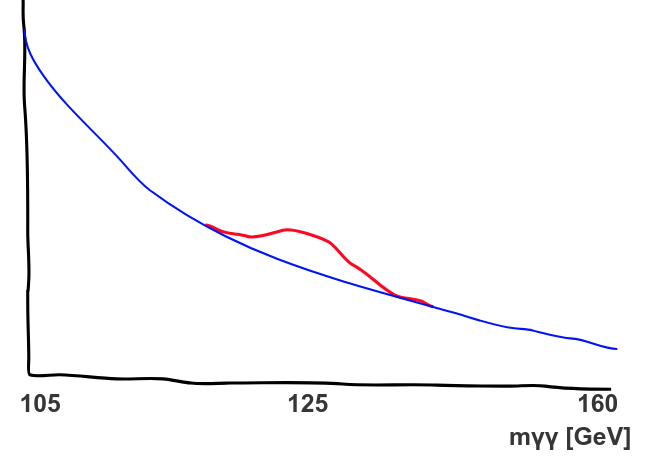
\includegraphics[width=0.8\textwidth]{Part3/Img/myysketch.png}
%\end{figure}
%\end{columns}
%    
%\end{frame}

\subsection{Higgs self-coupling constrain}

\begin{frame}{Signal extraction and results}

\begin{columns}
\column{0.6\textwidth}
\begin{itemize}
    \item Simultaneous fit of \textbf{$m_{\gamma\gamma}$} in the 4 analysis categories
    \begin{itemize}
        \item \textbf{\textcolor{HHred}{HH signal} (ggF + VBF) + \textcolor{HHred}{Single Higgs}}
        \begin{itemize}
            \item \textbf{from Monte Carlo} using Double-sided Crystal-Ball
        \end{itemize}
       \item \textbf{\textcolor{HHturquoise_d}{Continuum $\gamma\gamma$ + jets}}
       \begin{itemize}
           \item \textbf{fully data driven}
       \end{itemize}
    \end{itemize}
    \item \textbf{\textcolor{HHred}{No significant signal is observed}}
    \item 95\% CL upper limits on $\sigma_{ggF+VBF}$ of diHiggs as a function of $\kappa_{\lambda}$
\end{itemize}

\column{0.4\textwidth}
\begin{textblock*}{5cm}(13.3cm, 3.6cm) % {block width} (coords) 
   \textbf{\textcolor{HHred}{--------------}}
\end{textblock*}
\begin{figure}
    \centering
    \fcolorbox{gray}{HHwhite2}{
    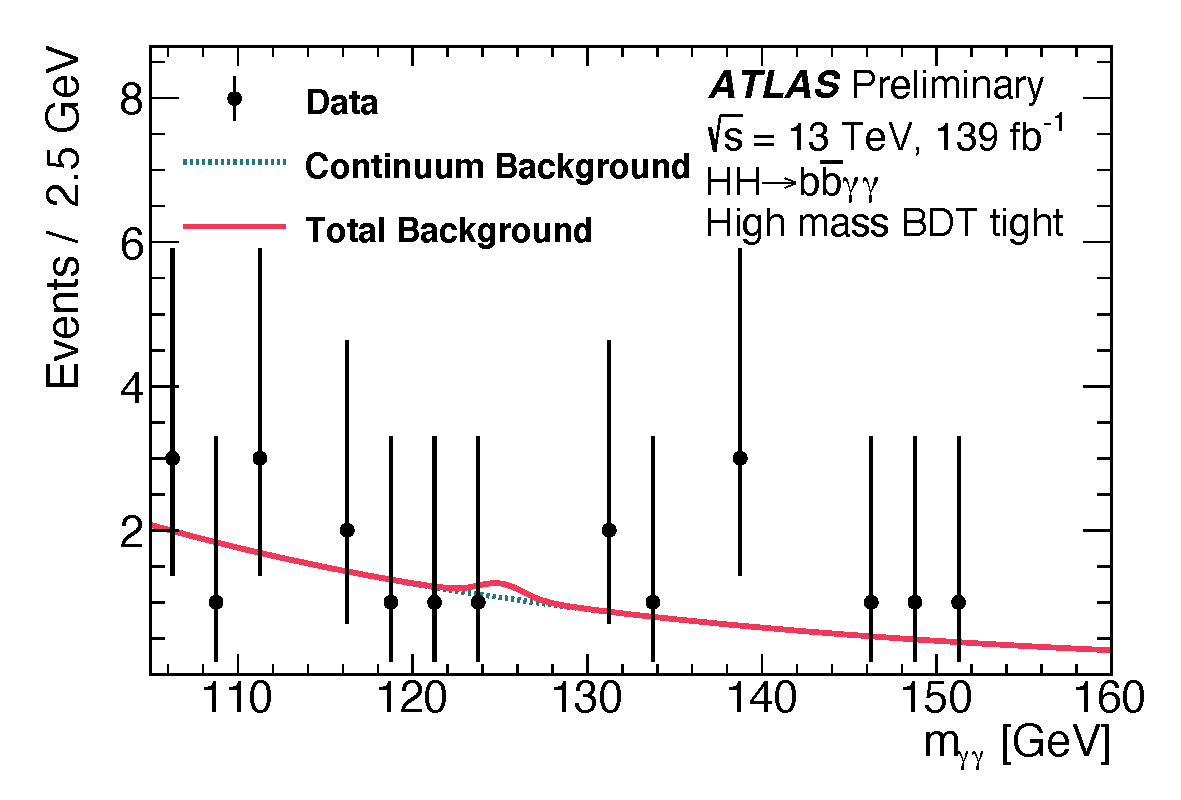
\includegraphics[width=1.\textwidth]{Part3/Img/myy_bkg_only_high_mass_tight_BDT.pdf}
    }
\end{figure}

\begin{center}
   \textcolor{gray}{ \textbf{most sensitive category}}
\end{center}

\end{columns}    
\end{frame}


\begin{frame}{Limits and $\kappa_{\lambda}$ constrain}
\setbeamercovered{transparent}
\begin{columns}
\column{0.4\textwidth}

\begin{textblock*}{5cm}(2cm,2.2cm) % {block width} (coords) 
   \textcolor{HHred}{\textbf{\href{https://atlas.web.cern.ch/Atlas/GROUPS/PHYSICS/CONFNOTES/ATLAS-CONF-2021-016}{ATLAS-CONF-2021-016}}}
\end{textblock*}

\begin{textblock*}{6cm}(8cm,4.5cm) % {block width} (coords) 
  \visible<2>{ \textcolor{HHred}{\Large\textbf{The world's best $\kappa_{\lambda}$ limit}}}
\end{textblock*}

\begin{figure}
    \centering
    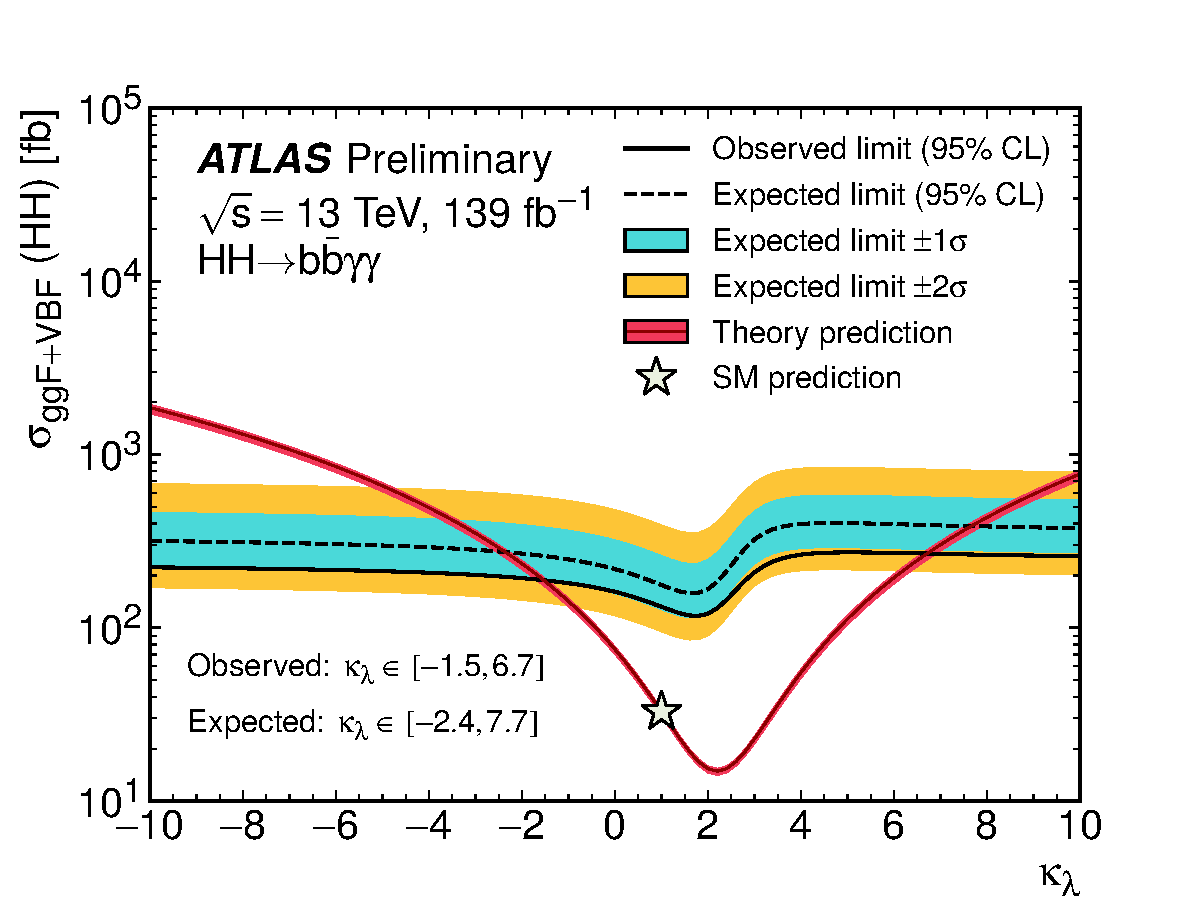
\includegraphics[width=1.1\textwidth]{Part3/Img/limit_yybb.pdf}
\end{figure}

\column{0.6\textwidth}

\begin{itemize}
    \item $\frac{\sigma_{HH}}{\sigma_{HH}^{SM}}$ limit: \textbf{\textcolor{HHred}{4.1}} (Exp. \textbf{5.5}) at 95\% CL
    \item $\kappa_{\lambda}$ constrain: \textbf{\textcolor{HHred}{[-1.5, 6.7]}} (Exp. \textbf{[-2.4, 7.7]})
    \onslide<3->{
    \item \textbf{Statistically limited}
    \begin{itemize}
        \item Systematic effect $\sim$ \textbf{4\%}
        \item Background modelling \& photon energy scale
    \end{itemize}
    }
    \onslide<4->{
    \pause
    \item \textbf{\textcolor{cadmiumorange}{5$\times$ improvement}} w.r.t 36 fb$^{-1}$
    \begin{itemize}
        \item Increased luminosity: 2$\times$
        \item \textbf{\textcolor{HHturquoise_d}{Analysis improvement: almost 3$\times$}}
        \begin{itemize}
            \item$m_{HH}$ categorization and MVA strategy (\textbf{80\%})
            \item $b$-jet energy calibration (\textbf{7\%})
            \item ...
        \end{itemize}
    \end{itemize}
    }
  %  \item HH$\to b\bar{b}\tau^+\tau^-$ $\frac{\sigma_{HH}}{\sigma_{HH}^{SM}}$ limit: \textcolor{HHred}{\textbf{4.7}} (Exp. \textbf{3.9})
\end{itemize}
\end{columns}
\end{frame}

\begin{frame}{CMS HH$\to b\bar{b}\gamma\gamma$ results}

\begin{columns}
\column{0.5\textwidth}

\begin{textblock*}{5cm}(2cm,2.2cm) % {block width} (coords) 
   \textcolor{HHred}{\textbf{\href{https://doi.org/10.1007/JHEP03(2021)257}{ JHEP03 (2021) 257}}}
\end{textblock*}

\begin{itemize}

    \item \textbf{\textcolor{structurColor}{Different analysis strategies}}
    \begin{itemize}
        \item 14 categories
        \begin{itemize}
            \item \textbf{MVAs output} and \textbf{$m_{b\bar{b}\gamma\gamma}^{*}$}
            \item \textbf{2 dedicated VBF categories} 
        \end{itemize}
        \item \textcolor{HHturquoise_d}{\textbf{2D fit}} $m_{\gamma\gamma}\times m_{b\bar{b}}$
    \end{itemize}
\end{itemize}

\column{0.5\textwidth}

\begin{table}[]
    \centering
    \begin{tabular}{lcc}
    \hline\hline
    & Expected & Observed \\
    \hline 
    CMS $\frac{\sigma_{HH}}{\sigma_{HH}^{SM}}$ limit & \textbf{5.2} & 7.7 \\
    CMS $\kappa_{\lambda}$ interval & \textbf{[-2.5, 8.2]} & [-3.3, 8.5] \\
    \hline 
    ATLAS $\frac{\sigma_{HH}}{\sigma_{HH}^{SM}}$ limit & \textbf{5.5} & 4.1 \\
    ATLAS $\kappa_{\lambda}$ interval & \textcolor{HHred}{\textbf{[-2.4, 7.7]}} & [-1.5, 6.7] \\ 
    \hline\hline
    \end{tabular}
    
\end{table}

%\begin{figure}
    %\centering
    %\fcolorbox{HHturquoise_d}{HHwhite2}{
    %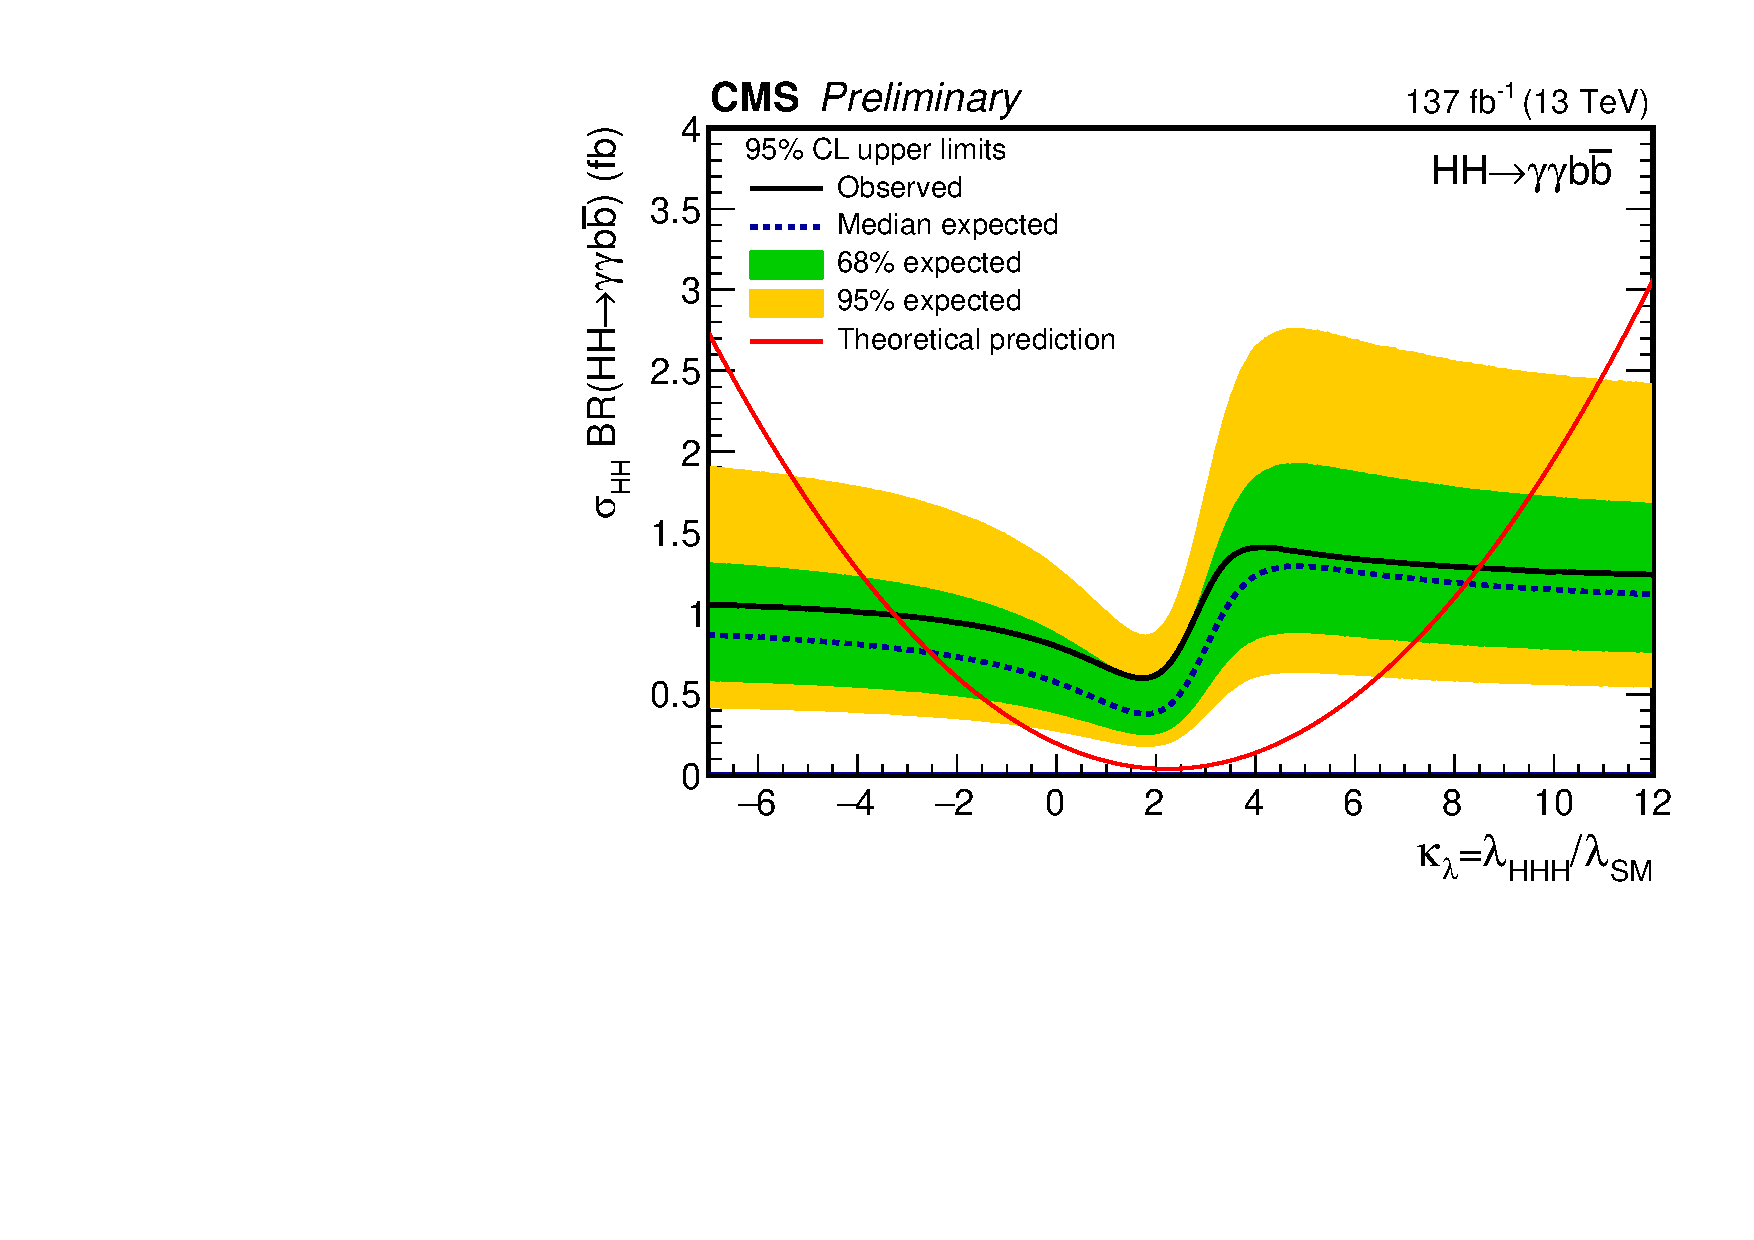
\includegraphics[width=1.\textwidth]{Part3/Img/CMS_kl_scan.pdf}
    %}
%\end{figure}
\end{columns}
\end{frame}



\section{Prospects at Run-3 and HL-LHC}

\begin{frame}{Content}
\label{content}
    \begin{columns}[t]
        \begin{column}{.5\textwidth}
            \tableofcontents[sections={1-5},currentsection]
        \end{column}
        \begin{column}{.5\textwidth}
            \tableofcontents[sections={6-},currentsection]
        \end{column}
    \end{columns}
\end{frame}

%\begin{frame}{Upgrade plans: Run-3 and HL-LHC}
%    \begin{figure}
%        \centering
%        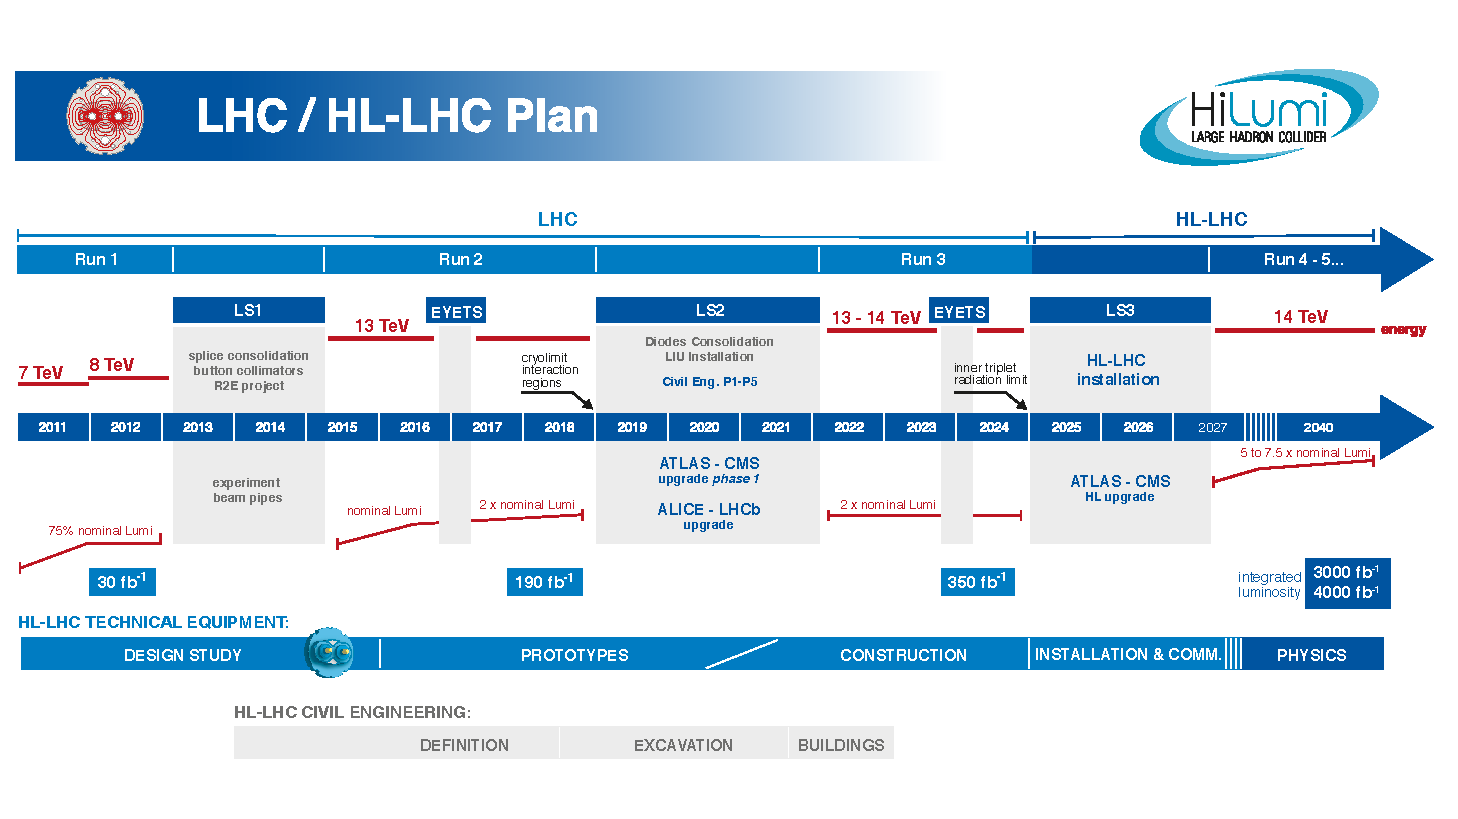
\includegraphics[width=0.6\textwidth]{Part2/Img/HL-LHC-plan-2021-1.pdf}
%    \end{figure}
%\begin{columns}
%\column{0.5\textwidth}  
%\begin{center}
%    \textbf{Run-3}
%\end{center}
%\begin{itemize}
%    \item $\sqrt{s}=$ 13.6 TeV
%    \item $\mathcal{L}_{int} \sim $ 300 fb$^{-1}$
%\end{itemize}
%\column{0.5\textwidth}  
%
%\begin{center}
%    \textbf{High-Luminosity LHC}
%\end{center}
%\begin{itemize}
%    \item $\sqrt{s}=$ 14 TeV
%    \item $\mathcal{L}_{int} \sim $  3000 fb$^{-1}$
%\end{itemize}
%
%\end{columns}
%\end{frame}


\subsection{Prospects at the end of Run-3}
\begin{frame}{Prospects at the end of Run-3}
\begin{textblock*}{5cm}(12cm,0.1cm) % {block width} (coords) 
   \textcolor{HHred}{\Large\textbf{my own work}}
\end{textblock*}
\begin{columns}
\column{0.6\textwidth}

\begin{itemize}
    \item \textbf{Run-2+Run-3}: $\mathcal{L}_{int} \sim $ 300 fb$^{-1}$, $\sqrt{s}$ = 13.6 TeV
    \begin{itemize}
        \item Detector upgrades: \textbf{no significant impact on HH$\to b\bar{b}\gamma\gamma$}
    \end{itemize}
\end{itemize}
\onslide<2->{
\begin{itemize}
    \item $\frac{\sigma_{HH}}{\sigma_{HH}^{SM}}$ limit: \textcolor{HHred}{\textbf{3.3}} (\textcolor{cadmiumorange}{\textbf{1.6$\times$ imp.}} w.r.t 139 fb$^{-1}$)
\end{itemize}
\begin{table}
    \centering
    \begin{tabular}{lcc}
    \hline\hline
        Scenario & 1$\sigma$ CI & 2$\sigma$ CI  \\
        \hline
        \textcolor{blue}{Run-2} & \textcolor{blue}{[-1.3, 6.4]} & \textcolor{blue}{[-2.9, 8]} \\
        Run-2+Run-3 & \textbf{[-0.7, 5.6]} & \textbf{[-1.9, 7]} \\
        \hline\hline
    \end{tabular}
\end{table}
}
\onslide<3->{

\underline{Potential improvements}:
\begin{itemize}
    \item \textbf{DNN categorization}: \textcolor{HHred}{\textbf{$\sim$10\%}}
    \item $m_{b \bar{b}}$ imp. with \textbf{kinematic fit}: \textcolor{HHred}{\textbf{2-5\%}}
    \item \textbf{Photon identification}: \textcolor{HHred}{\textbf{7\%}} (next part)
\end{itemize}
}
\column{0.4\textwidth}

\visible<2->{
\begin{figure}
    \centering
    \fcolorbox{HHred}{HHwhite2}{
    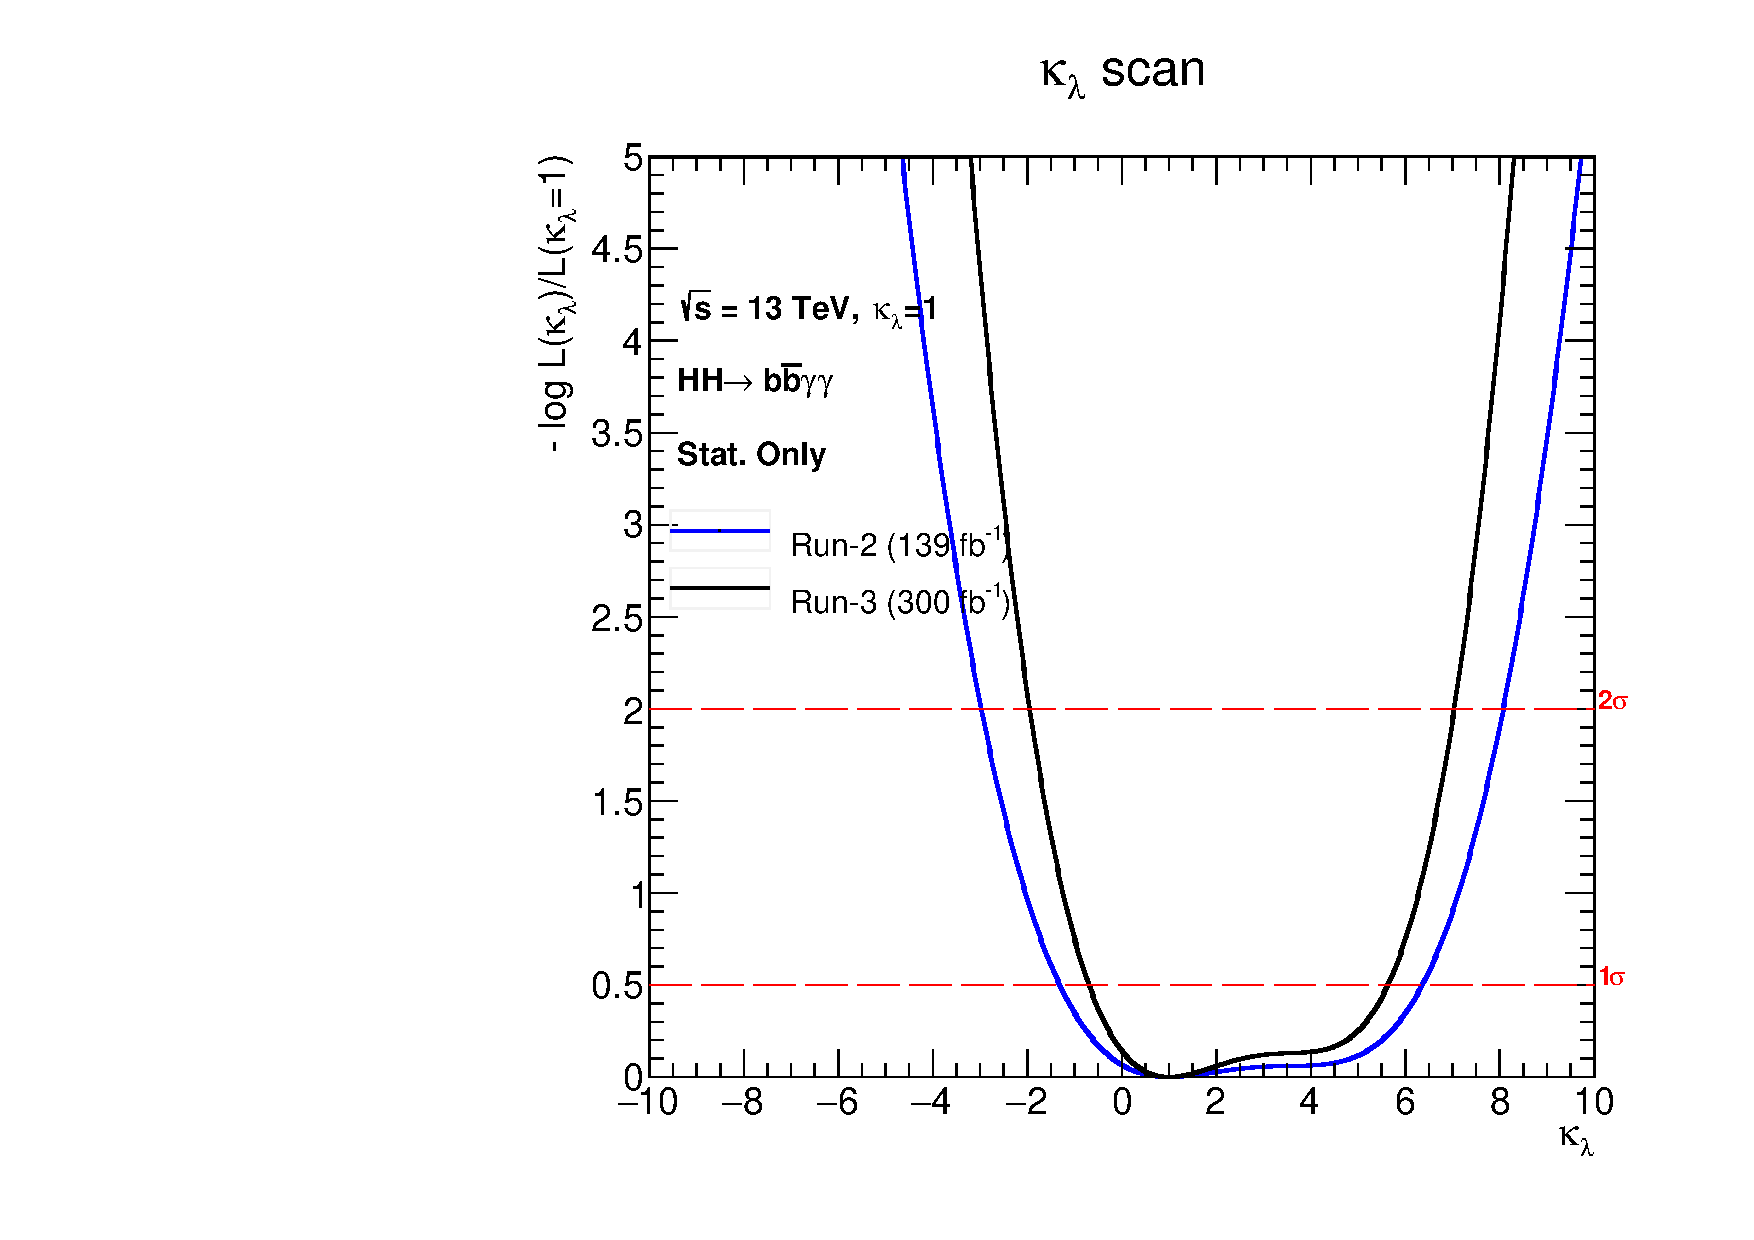
\includegraphics[width=1\textwidth]{Part4/Img/likelihood_subplot_Run3.pdf}
    }
\end{figure}
}
\end{columns}
\end{frame}

\subsection{Prospects at HL-LHC}
\begin{frame}{Prospects at HL-LHC}
\begin{textblock*}{5cm}(12cm,0.1cm) % {block width} (coords) 
   \textcolor{HHred}{\Large\textbf{my own work}}
\end{textblock*}
\begin{columns}
\column{0.4\textwidth}

\begin{figure}
    \begin{overprint}
    %\onslide<1>\centering\fcolorbox{HHturquoise_d}{HHwhite2}{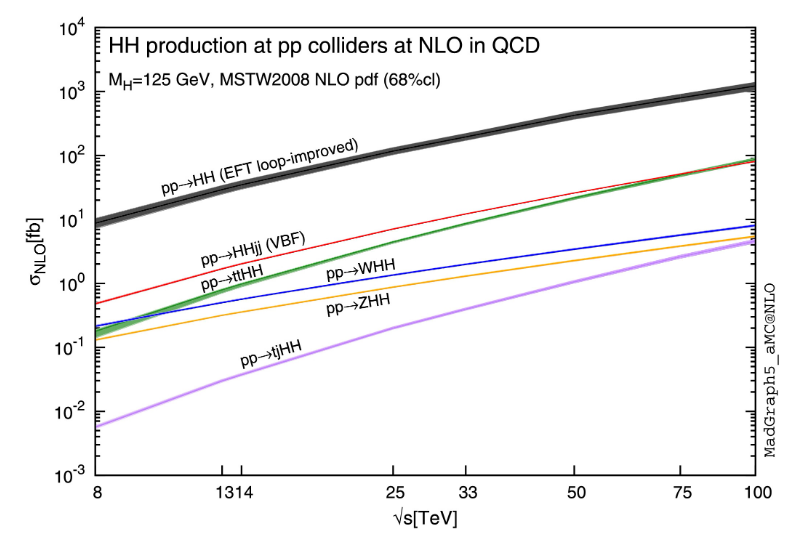
\includegraphics[width=1\textwidth]{Part1/Img/HH_XSec_as_S.png}}
    \onslide<2->\centering\fcolorbox{HHred}{HHwhite2}{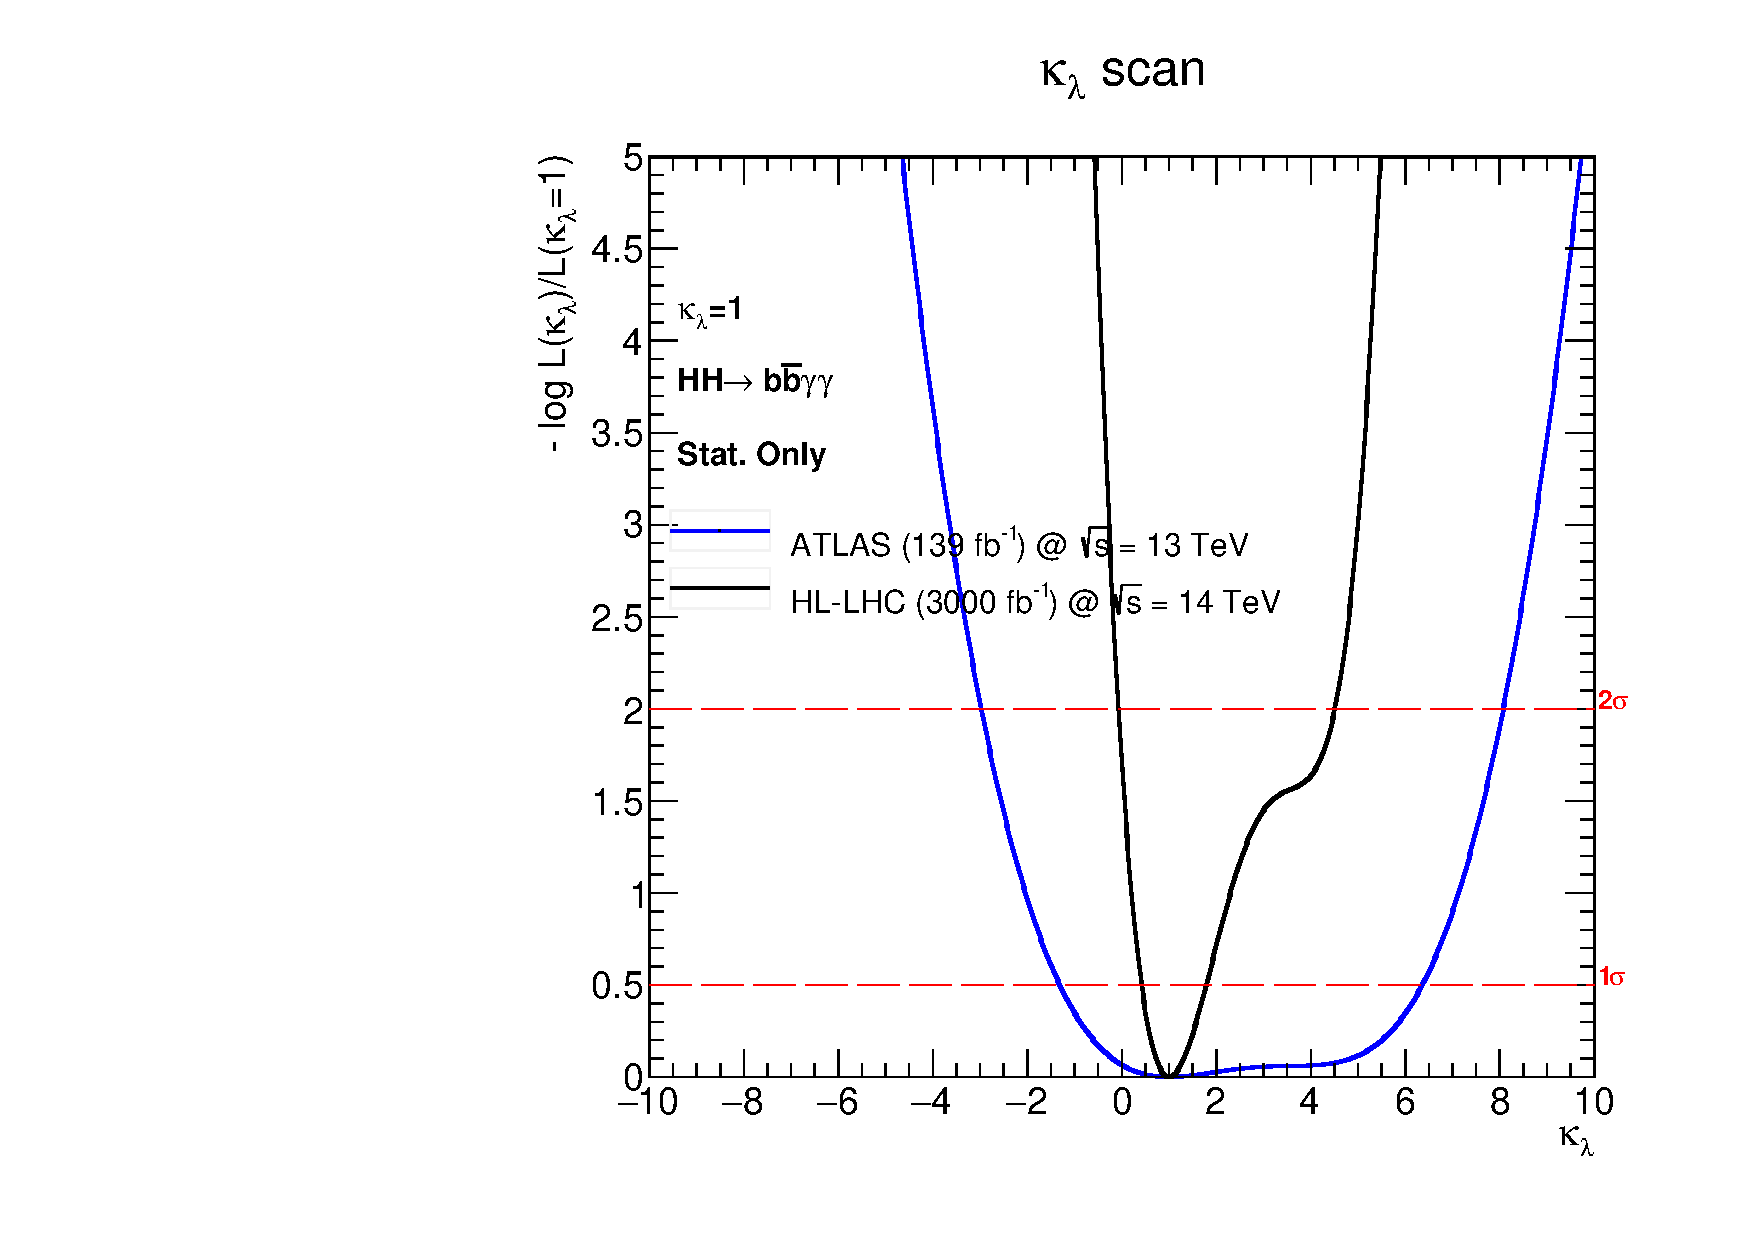
\includegraphics[width=1\textwidth]{Part4/Img/likelihood_subplot_14TeV.pdf}}
   \end{overprint}
\end{figure}


\column{0.6\textwidth}
\begin{itemize}
    \item \textbf{HL-LHC: \textcolor{HHturquoise_d}{$\sim$3000 fb$^{-1}$} at \textcolor{HHturquoise_d}{14 TeV}}
    \onslide<2->{
    \item Detector upgrades: \textbf{mitigate higher pileup effects} 
    \item European strategy: extrapolation from 36 fb$^{-1}$
    }
\end{itemize}
\onslide<2->{
\begin{table}[]
    \centering
    \begin{tabular}{lcc}
        \hline\hline
        Scenario & 1$\sigma$ CI & 2$\sigma$ CI  \\
        \hline
        \textcolor{blue}{European strategy} & \textcolor{blue}{[-0.1, 2.4]} & \textcolor{blue}{[-1.1, 8.1]} \\
        My Extra. to HL-LHC & \textbf{[0.4, 1.8]} & \textbf{[-0.1, 4.4]} \\
        \hline\hline
    \end{tabular}
\end{table}
}

\end{columns}    
\end{frame}

\begin{frame}{Prospects at HL-LHC}
\begin{textblock*}{5cm}(12cm,0.1cm) % {block width} (coords) 
   \textcolor{HHred}{\Large\textbf{my own work}}
\end{textblock*}
\begin{columns}
\column{0.4\textwidth}

\begin{figure}
  \centering
  \fcolorbox{HHturquoise_d}{HHwhite2}{
   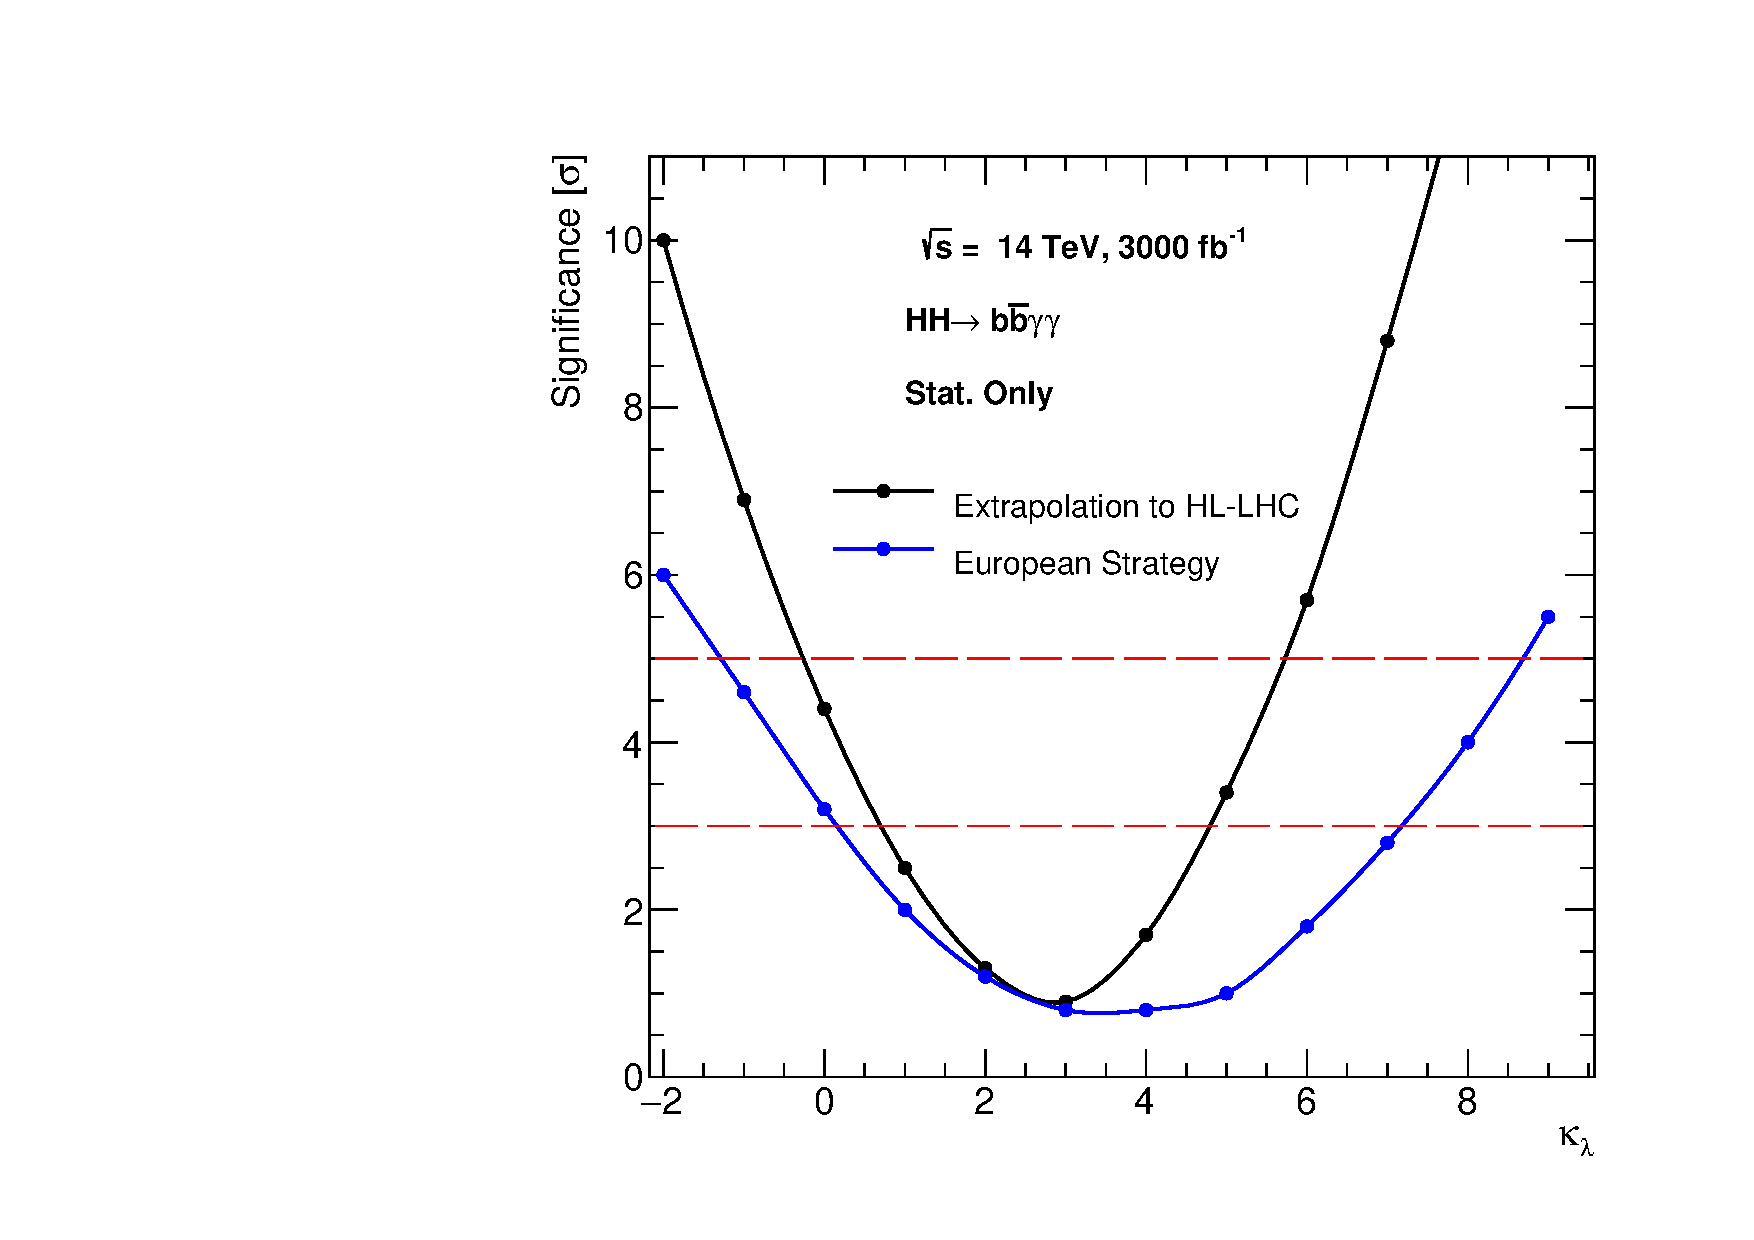
\includegraphics[width=1\textwidth]{Part4/Img/sig.pdf}
   }
\end{figure}


\column{0.6\textwidth}
\begin{itemize}
    \item \textbf{HL-LHC: \textcolor{HHturquoise_d}{$\sim$3000 fb$^{-1}$} at \textcolor{HHturquoise_d}{14 TeV}}
    \item Detector upgrades: \textbf{mitigate higher pileup effects} 
    \item European strategy: extrapolation from 36 fb$^{-1}$
\end{itemize}

\begin{table}[]
    \centering
    \begin{tabular}{lc}
        \hline\hline
        Scenario & Significance [$\sigma$]  \\
        \hline
        \textcolor{blue}{European strategy} & \textcolor{blue}{2.1} \\
        My Extra. to HL-LHC & \textbf{2.5} \\
        \hline\hline
    \end{tabular}
\end{table}

\begin{center}
    \textbf{\textcolor{HHturquoise_d}{Similar performances for SM} } \\
    \textbf{\textcolor{HHred}{Large gain at high $\kappa_{\lambda}$}}
\end{center}

\end{columns}  
\end{frame}

\section{Interpretation using Effective Field Theory}

\begin{frame}{Content}
\label{content}
    \begin{columns}[t]
        \begin{column}{.5\textwidth}
            \tableofcontents[sections={1-5},currentsection]
        \end{column}
        \begin{column}{.5\textwidth}
            \tableofcontents[sections={6-},currentsection]
        \end{column}
    \end{columns}
\end{frame}

\subsection{Di-Higgs and Effective Field Theory}
\begin{frame}{Effective Field Theory (EFT)}
\begin{itemize}
    \item Search for new physics at large energy scale ($\Lambda$) in a \textcolor{HHred}{\textbf{model independent}} way
    \item At large scale ($\Lambda >> v$), BSM decouples from SM
    \begin{equation*}
   \mathcal{L}=\mathcal{L}_{S M}+\mathcal{L}^{5}+\mathcal{L}^{6}+\mathcal{L}^{7}+\ldots, \quad \textcolor{HHblue}{\mathcal{L}^{d}=\sum_{i=1}^{n_{d}} \frac{c_{i}^{d}}{\Lambda^{d-4}} \mathcal{O}_{i}^{d}} \quad \text{for} \ d>4
   \end{equation*}
   \item \textcolor{HHred}{\textbf{Cross-section}} (and \textbf{decay width}) can be split
   \begin{equation*}
       \sigma = \textcolor{HHyellow}{\sigma_{SM}} + \textcolor{HHred}{\sigma_{int}} + \textcolor{HHturquoise_d}{\sigma_{BSM}}
   \end{equation*}
   \begin{equation*}
    \frac{\sigma}{\sigma_{SM}} = \textcolor{HHyellow}{1} + \textcolor{HHred}{\sum_{i} a_i \cdot c_i} + \textcolor{HHturquoise_d}{\sum_{i,j} b_{ij} \cdot c_i \cdot c_j}
   \end{equation*}
   \item \textbf{Standard Model Effective Field Theory} (SMEFT) in \textbf{Warsaw} basis with \textbf{d = 6} and \textbf{$\Lambda = $ 1 TeV}
\end{itemize}
\end{frame}

\begin{frame}{Di-Higgs and EFT}
\begin{textblock*}{5cm}(12.3cm, 2.3cm) % {block width} (coords) 
   \visible<1>{\textcolor{HHred}{ $c_{H}$}}
\end{textblock*}
\begin{textblock*}{5cm}(12.2cm, 3.2cm) % {block width} (coords) 
    \visible<1>{\textcolor{HHturquoise_d}{$c_{H\square}$}}
\end{textblock*}
\begin{textblock*}{5cm}(14cm, 5cm) % {block width} (coords) 
     \visible<1>{\textcolor{cadmiumorange}{$c_{uH}$}}
\end{textblock*}
\begin{textblock*}{5cm}(9.3cm, 4.8cm) % {block width} (coords) 
     \visible<1>{\textcolor{applegreen}{$c_{tG}$}}
\end{textblock*}

\begin{textblock*}{5cm}(12.2cm, 3.2cm) % {block width} (coords) 
    \visible<2>{\textcolor{HHred}{\textbf{Interference}}}
\end{textblock*}
\begin{columns}
\column{0.5\textwidth}    
\begin{itemize}
        \item 5 operators are relevant for di-Higgs
        \begin{itemize}
            \item \textcolor{HHred}{$c_H$} and \textcolor{HHturquoise_d}{$c_{H\square}$} modify the Higgs self-coupling $\kappa_{\lambda}$
            \begin{equation*}
                \kappa_{\lambda} = 1 - 2\frac{v^4}{m_{H}^2}\cdot \textcolor{HHred}{c_{H}} + 3\left(\textcolor{HHturquoise_d}{c_{H\square}} - \frac{\textcolor{HHyellow}{c_{HD}}}{4}\right)
            \end{equation*}
            \item \textcolor{cadmiumorange}{$c_{uH}$} and \textcolor{applegreen}{$c_{tG}$} modify the top quark interaction to the Higgs and gluons.
            \begin{equation*}
                \kappa_{t} = 1 + \left(\textcolor{HHturquoise_d}{c_{H\square}} - \frac{\textcolor{HHyellow}{c_{HD}}}{4}\right) - \frac{v^3}{\sqrt{2m_{t}}}\cdot \textcolor{cadmiumorange}{c_{uH} }
            \end{equation*}
            \item \textbf{\textcolor{orange}{$c_{HG}$}}, modify the Higgs coupling to gluons (\textbf{not considered}). 
        \end{itemize}
    \end{itemize} 
\column{0.5\textwidth}    
    
\begin{figure}
    \begin{overprint}
    \onslide<1>\centering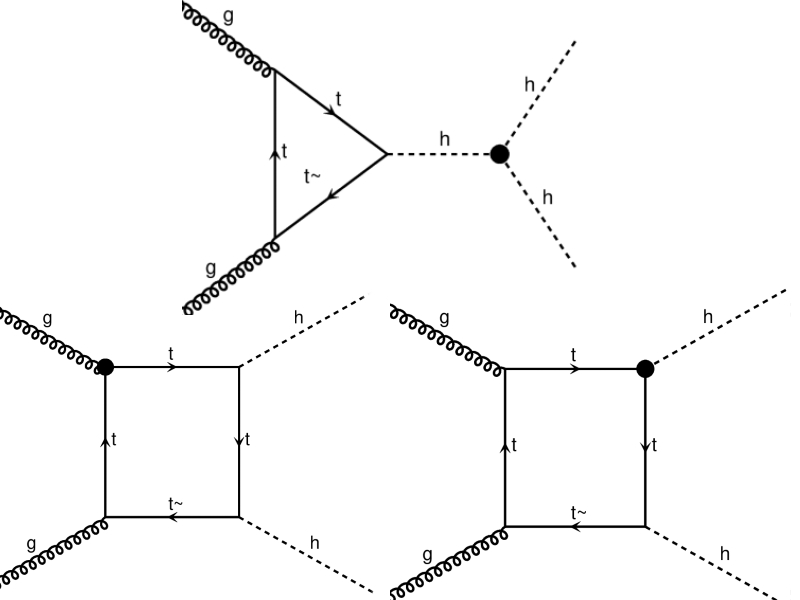
\includegraphics[width=1.\textwidth]{Part5/Img/EFT_feyns.jpg}
     \onslide<2>\centering\includegraphics[width=1\textwidth]{Part5/Img/EFT_suplot.pdf}
    \end{overprint}
\end{figure}    
    
\end{columns}
    
\end{frame}

\begin{frame}{Cross-section parameterization in HH $\to b\bar{b}\gamma\gamma$}

\begin{textblock*}{5cm}(12cm,0.1cm) % {block width} (coords) 
   \textcolor{HHred}{\Large\textbf{my own work}}
\end{textblock*}
\begin{columns}
\column{0.5\textwidth}

\begin{itemize}
    \item $b\bar{b}\gamma\gamma$ measurements in two phase space regions
    \begin{itemize}
        \item \textcolor{HHred}{\textbf{High mass}} ($m_{HH} > $ 350 GeV) 
        \item \textcolor{HHturquoise_d}{\textbf{Low mass}} ($m_{HH} < $ 350 GeV)
    \end{itemize}
    \item ggF HH cross-section parameterized as function of the Wilson coefficients
\end{itemize}

\column{0.5\textwidth}

%\begin{table}[]
%    \begin{tabular}{ll}
%    \hline\hline
%    Region  & $\sigma/\sigma_{SM}$ \\
%    \hline
%    High mass &  - 0.19 $\cdot$ $c_{H\square}$ + 0.02 $\cdot$ $c_{H\square}^2$  + \textcolor{HHred}{0.31 $\cdot$ $c_{H}$}\\
%    & + 0.03 $\cdot$ $c_{H}^2$ + 0.24 $\cdot$ $c_{uH}$ + 0.03 $\cdot$ $c_{uH}^2$ \\
%    & - \textcolor{HHred}{0.30 $\cdot$ $c_{tG}$} + 0.05 $\cdot$ $c_{tG}^2$ - 0.04 $\cdot$ $c_{H}$ $\cdot$ $c_{H\square}$ \\
%   & + 0.04 $\cdot$ $c_{H}$ $\cdot$ $c_{uH}$ - 0.06 $\cdot$ $c_{H}$ $\cdot$ $c_{tG}$ \\
%   & - 0.05 $\cdot$ $c_{H\square}$ $\cdot$ $c_{uH}$ + 0.04 $\cdot$ $c_{H\square}$ $\cdot$ $c_{tG}$ \\
%   & - 0.06 $\cdot$ $c_{uH}$ $\cdot$ $c_{tG}$ \\ 
%   \hline
%    Low mass &
%    - 0.38 $\cdot$ $c_{H\square}$ + 0.05 $\cdot$ $c_{H\square}^2$ + \textcolor{HHturquoise_d}{0.79 $\cdot$ $c_{H}$} \\
%  & +  0.22 $\cdot$ $c_{H}^2$ + 0.28 $\cdot$ $c_{uH}$ +  0.02 $\cdot$ $c_{uH}^2$ \\
%  & - \textcolor{HHturquoise_d}{0.16 $\cdot$ $c_{tG}$} + 0.02 $\cdot$ $c_{tG}^2$  - 0.21 $\cdot$ $c_{H}$ $\cdot$ $c_{H\square}$ \\
%  & + 0.14 $\cdot$ $c_{H}$ $\cdot$ $c_{uH}$ + 0.09 $\cdot$ $c_{H}$ $\cdot$ $c_{tG}$ \\
%  & - 0.07 $\cdot$ $c_{H\square}$ $\cdot$ $c_{uH}$ - 0.03 $\cdot$ $c_{H\square}$ $\cdot$ $c_{tG}$ \\
%  & + 0.03 $\cdot$ $c_{uH}$ $\cdot$ $c_{tG}$ \\
%  \hline\hline
%    \end{tabular}
%\end{table}

\begin{textblock*}{5cm}(12.5cm, 8cm) % {block width} (coords) 
    \textbf{\textcolor{HHred}{High mass}}
\end{textblock*}
\begin{textblock*}{5cm}(9.5cm, 8cm) % {block width} (coords) 
    \textbf{\textcolor{HHturquoise_d}{Low mass}}
\end{textblock*}
\begin{figure}
    \centering\includegraphics[width=1.\textwidth]{Part5/Img/a_i_total.pdf}
\end{figure}   


\end{columns} 
\end{frame}

%\begin{frame}{Interference impact on HH cross-section}
%\begin{textblock*}{5cm}(8.8cm, 8.5cm) % {block width} (coords) 
%    \textbf{\textcolor{HHred}{High mass}}
%\end{textblock*}
%\begin{textblock*}{5cm}(5.5cm, 8.5cm) % {block width} (coords) 
%    \textbf{\textcolor{HHturquoise_d}{Low mass}}
%\end{textblock*}
%\begin{figure}
%    \centering\includegraphics[width=0.6\textwidth]{Part5/Img/a_i_total.pdf}
%\end{figure}   
%\end{frame}

\subsection{EFT coefficients constrains}

\begin{frame}{Results}
\begin{textblock*}{5cm}(12cm,0.1cm) % {block width} (coords) 
   \textcolor{HHred}{\Large\textbf{my own work}}
\end{textblock*}
%\begin{textblock*}{5cm}(9.8cm, 3cm) % {block width} (coords) 
%    $c_{H}$
%\end{textblock*}
%\begin{textblock*}{5cm}(9.8cm, 4cm) % {block width} (coords) 
%    $c_{H\square}$
%\end{textblock*}

\begin{textblock*}{5cm}(9.8cm, 5.8cm) % {block width} (coords) 
     $vec_{0}$
\end{textblock*}
\begin{textblock*}{5cm}(9.8cm, 7.8cm) % {block width} (coords) 
     $vec_{1}$
\end{textblock*}


%\begin{textblock*}{5cm}(1cm, 5.5cm) % {block width} (coords) 
%    \onslide<2->{\textbf{\textcolor{HHred}{again,
%    HH$\to b\bar{b}\gamma\gamma$  \\ results}}}
%\end{textblock*}

\begin{itemize}
    \item Not sensitive to all coefficients (\textbf{two mass regions}) \\
    $\to$ Need \textcolor{HHred}{\textbf{sensitivity estimate}} to find relevant ones
    \begin{itemize}
        \item Look at the eigenvectors of the inverse covariance matrix of Wilson coefficients
    \end{itemize}
\end{itemize}
\begin{table}[]
    \centering
    \begin{tabular}{lcc}
    \hline\hline
    & Eigenvalue & Eigenvector \\
    \hline
  $vec_{0}$ & \textcolor{HHred}{0.0523}  &  - 0.582 $\cdot$ $c_{H}$ + 0.363 $\cdot$ $c_{H\square}$ - 0.456 $\cdot$ $c_{uH}$ + 0.567 $\cdot$ $c_{tG}$ \\ \hline
  $vec_{1}$ &  \textcolor{HHred}{0.0001}  &  - 0.696 $\cdot$ $c_{H}$ + 0.182 $\cdot$ $c_{H\square}$ + 0.206 $\cdot$ $c_{uH}$ - 0.663 $\cdot$ $c_{tG}$ \\ \hline
  $vec_{3}$ & -0.0000 &  - 1.025 $\cdot$ $c_{H}$ - 1.947 $\cdot$ $c_{H\square}$ + 0.702 $\cdot$ $c_{uH}$ + 0.759 $\cdot$ $c_{tG}$ \\ \hline
  $vec_{4}$ & -0.0000 &  - 0.235 $\cdot$ $c_{H}$ - 0.006 $\cdot$ $c_{H\square}$ + 0.977 $\cdot$ $c_{uH}$ + 0.549 $\cdot$ $c_{tG}$ \\ \hline
   \hline
    \end{tabular}
\end{table}

%\begin{itemize}
    %\item Simultaneous fit of the 4 Wilson coefficients
%\end{itemize}

%\begin{table}[]
%    \centering
%    \begin{tabular}{lccc}
%    \hline\hline
%    Coeff. & measured & measured & expected \\
%    & value & error & error \\
%    \hline
%    $c_{H}$ & -4.3 & $^{+9.3}_{-5.7}$ & $^{+10.4}_{-9.6}$ \\
%    \hline 
%    $c_{H\square}$ & -1.7 & $^{+11.7}_{-8.3}$ & $^{+9.8}_{-10.7}$ \\
%    \hline 
%    $c_{uH} $ & -1.6 & $^{+11.6}_{-8.3}$ & $^{+10.5}_{-9.5}$ \\
%    \hline 
%    $c_{tG}$ & 0.4 & $^{+6.4}_{-6.2}$ & $^{+9.6}_{-10.4}$ \\
%    \hline\hline
%    \end{tabular}
%\end{table}

%\onslide<2->{
%\begin{table}[]
%    \centering
%    \begin{tabular}{lc}
%    \hline\hline
%         & value \\
%    \hline    
%        $\kappa_{\lambda}$ & 2.72 \\
%        $\kappa_t$ & 1 \\
%    \hline\hline    
%    \end{tabular}
%\end{table}
%}
\begin{columns}
\column{0.6\textwidth}
\begin{itemize}
    \item Measurement of most sensitive eigenvectors
\end{itemize}

\begin{table}[]
    \centering
    \begin{tabular}{lc}
    \hline\hline
         & expected error \\
    \hline    
        $vec_{0}$ & $^{+3.9}_{5.1}$ \\
        $vec_{1}$ & $^{+80.8}_{-102.1}$ \\
    \hline \hline    
    \end{tabular}
\end{table}

\begin{itemize}
    \item Additional measurement regions, combination with other measurements (Higgs, Top) needed
    \item \textcolor{HHred}{\textbf{Work in progress}}
\end{itemize}
\column{0.4\textwidth}

\begin{figure}
    \centering
    \includegraphics[width=0.85\textwidth]{Part5/Img/correlationHist_fit_eigvec_asimov.pdf}
\end{figure}

\end{columns}    
\end{frame}

{
\usebackgroundtemplate{\includegraphics[width=1.03\paperwidth]{Img/figaux_01}}
\begin{frame}
\end{frame}
}

\section{Photon identification using Convolutional Neural Network}

\begin{frame}{Content}
\label{content}
    \begin{columns}[t]
        \begin{column}{.5\textwidth}
            \tableofcontents[sections={1-5},currentsection]
        \end{column}
        \begin{column}{.5\textwidth}
            \tableofcontents[sections={6-},currentsection]
        \end{column}
    \end{columns}
\end{frame}

\subsection{Photon identification with Neural Network}
\begin{frame}{EM calorimeter and $\gamma$ object}
\begin{columns}
\column{0.4\textwidth}
\begin{figure}
    \centering
    \includegraphics[width=1.\textwidth]{Part6/Img/EM.png}
\end{figure}
\column{0.6\textwidth}

\begin{itemize}
    \item \textcolor{structurColor}{\textbf{3 layers}} with different \textbf{cell size} (+ Presampler)
    \item \textbf{$N_{\eta}\times N_{\phi}$ cluster} contains most $\gamma$ energy
    \pause
    \item \textcolor{HHturquoise_d}{\textbf{Shower shapes}} (SS) quantities ($\sim$ 11) evaluated from 7$\times$11 cluster
    \begin{itemize}
        \item \textbf{Lateral} \& \textbf{longitudinal} EM shower
        \item \textbf{Discriminate between} \textcolor{HHred}{\textbf{prompt photons}} and \textcolor{HHblue}{\textbf{background photons}} (QCD jets)
    \end{itemize}
\end{itemize}
\visible<2-3>{
\begin{figure}
    \centering
    \includegraphics[width=0.8\textwidth]{Part6/Img/ShowerShapes.png}
\end{figure}
}
\pause
\begin{itemize}
    \item Current identification relies on SS: \textbf{cut-based algorithm}
    \item \textcolor{HHred}{\textbf{Propose improvement using Neural Network}}
\end{itemize}
\end{columns} 
\end{frame}

\begin{frame}{Photon identification with Neural Network}
\begin{textblock*}{5cm}(11.6cm, 7.8cm) % {block width} (coords) 
\visible<3>{
   $\eta$ direction
} 
\end{textblock*}
\begin{textblock*}{5cm}(10cm, 4.5cm)
\visible<3>{
   \rotatebox{90}{$\phi$ direction}
} 
\end{textblock*}
\begin{textblock*}{5cm}(14.5cm, 3cm) % {block width} (coords) 
\visible<3>{
   $\frac{E_{\text{cell}}}{E_{\text{cluster}}}$
} 
\end{textblock*}
\begin{columns}
\column{0.6\textwidth}    
\begin{itemize}
    \item Global shower shapes (High level) \\
    \textbf{Cut-based $\to$ DNN}
    \begin{itemize}
        \item \textcolor{HHred}{\textbf{Limited performance}} (small features space)
    \end{itemize}
    \pause
    \item Solution: \textbf{\textcolor{HHturquoise_d}{breakdown to cell level}} (Low level)
    \begin{itemize}
        \item Scale up features space dimensionality
        \begin{itemize}
            \item \textbf{Generate more variables}
            \item \textbf{Correlation between cells}
        \end{itemize} 
    \end{itemize}
    \pause
    \item \textcolor{structurColor}{\textbf{Convolutional Neural Network (CNN)}}
    \begin{itemize}
        \item Photon cluster represented as an image
    \end{itemize}
    \item Photon identification (ID) using images from the 3 layers 
\end{itemize}    
\column{0.4\textwidth}  

\visible<3>{
\begin{center}
    7$\times$11 cluster from 2$^{nd}$ layer
\end{center}
\begin{figure}
        \centering
        \includegraphics[width=0.8\textwidth]{Part6/Img/7_11_cluster.png}
\end{figure}
}

\end{columns}
\end{frame}

\begin{frame}{Convolutional Neural Network strategy and training}
\begin{textblock*}{5cm}(12cm,0.1cm) % {block width} (coords) 
   \textcolor{HHred}{\Large\textbf{my own work}}
\end{textblock*}
\begin{columns}
\column{0.6\textwidth}    
\begin{itemize}
    \item \textcolor{HHred}{\textbf{Prompt photons}}: inclusive $\gamma$+jets events
    \item \textcolor{HHblue}{\textbf{Background photons}}: QCD di-jet events 
    %\item + truth matching 
    \pause
    \item Images from \textbf{7$\times$11 windows} 
    \begin{itemize}
        \item \textbf{Energy independent algorithm}
        \item Image pixel = cell energy fraction
    \end{itemize}
    \pause
    \item \textbf{Inclusive training} ($E_T$, $|\eta| < $ 2.4, conversion type)
    \item \textbf{Trained on Monte Carlo}
    \end{itemize}
    \pause
    \begin{itemize}
        \item CNN \textcolor{HHred}{\textbf{over-performs}} the cut-based algorithm
    \end{itemize}
    
    
\column{0.4\textwidth} 

\begin{figure}
    \begin{overprint}
    \onslide<1-3>\centering\includegraphics[width=1.1\textwidth]{Part6/Img/CNN_Idea2.pdf}
    \onslide<4>\centering\fcolorbox{HHred}{HHwhite2}{\includegraphics[width=1\textwidth]{Part6/Img/ROC_UnConverted.png}}
    \end{overprint}
\end{figure}
\end{columns}
\end{frame}

\subsection{Photon identification efficiency}
\begin{frame}{Photon identification efficiency}
\begin{textblock*}{5cm}(12cm,0.1cm) % {block width} (coords) 
   \textcolor{HHred}{\Large\textbf{my own work}}
\end{textblock*}
\begin{columns}
\column{0.6\textwidth}

\begin{itemize}
    \item Identification efficiency with \textcolor{HHred}{\textbf{Radiative Z method}} 
    \begin{itemize}
        \item Z$\to ll\gamma$ ($l$=$e$,$\mu$), \textbf{as a signal}
        \item Z$\to ll$+jet ($l$=$e$,$\mu$), \textbf{as a background}
        \item \textbf{2017 data} (43.6 fb$^{-1}$)
    \end{itemize}
    \item Efficiency as
    \begin{equation*}
        \epsilon_{ID} = \frac{N^{\text{after ID}} \times P^{\text{after ID}}}{N^{\text{before ID}} \times P^{\text{before ID}}}
    \end{equation*}
    \onslide<2->{
    \item Purity estimated with \textcolor{HHturquoise_d}{\textbf{template fit of $m_{ll\gamma}$}}
    }
    %\begin{itemize}
    %    \item signal template \textbf{from Monte Carlo}
    %    \item \textbf{second-order polynomial function} for background
    %    \item \textcolor{structurColor}{\textbf{$E_T^{\gamma} > $ 30 GeV, pure photon samples}} 
    %\end{itemize}
    \onslide<2->{
    \item \textcolor{HHred}{\textbf{Over-performs}} the cut-based algorithm
    \begin{itemize}
        \item Out-of-sample validation: \textbf{different event topology}
        \item \textbf{Good data-MC agreement}
    \end{itemize}
    }
\end{itemize}

\column{0.4\textwidth}

\begin{figure}
    \begin{overprint}
    %\onslide<2>\centering\fcolorbox{HHturquoise_d}{HHwhite2}{\includegraphics[width=1.\textwidth]{Part6/Img/UnConvertedllg_Before_ID_Bin_1.png}}
   % \onslide<2>\centering\fcolorbox{structurColor}{HHwhite2}{\includegraphics[width=1.\textwidth]{Part6/Img/UnConvertedllg_After_ID_Bin_1.png}}
    \onslide<2->\centering\fcolorbox{HHred}{HHwhite2}{\includegraphics[width=1.\textwidth]{Part6/Img/Tight_Inc_vs_Tight_CNN__UnConverted_Iso_tight_Wgt_ETA_Bin_1.png}}
    \end{overprint}
\end{figure}

\end{columns}
\end{frame}

%\subsection{Impact on HH$\to b\bar{b}\gamma\gamma$}
\begin{frame}{Impact on HH$\to b\bar{b}\gamma\gamma$ analysis}
\begin{textblock*}{5cm}(12cm,0.1cm) % {block width} (coords) 
   \textcolor{HHred}{\Large\textbf{my own work}}
\end{textblock*}
\begin{columns}
\column{0.6\textwidth}    
\begin{itemize}
    \item CNN applied to photons from HH$\to b\bar{b}\gamma\gamma$ signal
    \begin{itemize}
   
        \item \textcolor{HHturquoise_d}{\textbf{Efficiency close to 100\%}}
    
   
        \item \textbf{15\% improvement in signal acceptance}
    
    \end{itemize}
    
    \item CNN applied to photons from continuum $\gamma\gamma$+jets
    
    \begin{itemize}
    
        \item \textcolor{HHturquoise_m}{\textbf{high $\gamma\gamma$ purity}}
        \item \textbf{15\% increase in statistics}
        \item \textbf{Reduce background modelling systematics}
    
    \end{itemize}

    \item \textbf{\textcolor{HHred}{$\sim$ 7.3\%} improvement in analysis significance}
    
    
\end{itemize}
\column{0.4\textwidth}    

\begin{figure}
    \begin{overprint}
    \onslide<1->\centering\fcolorbox{HHturquoise_d}{HHwhite2}{\includegraphics[width=1\textwidth]{Part6/Img/Eff_Tight_All_Inclusive_Tight_E_Sig.pdf}}
   % \onslide<3>\centering\fcolorbox{HHturquoise_d}{HHwhite2}{\includegraphics[width=1\textwidth]{Part6/Img/Eff_Tight_All_Inclusive_Tight_M_Sig.pdf}}
    %\onslide<5>\centering\fcolorbox{HHturquoise_m}{HHwhite2}{\includegraphics[width=1\textwidth]{Part6/Img/Eff_Tight_All_Inclusive_Tight_E_Bkg.pdf}}
    %\onslide<6>\centering\fcolorbox{HHturquoise_m}{HHwhite2}{\includegraphics[width=1\textwidth]{Part6/Img/Eff_Tight_All_Inclusive_Tight_M_Bkg.pdf}}
    \end{overprint}
\end{figure}
\end{columns}

\end{frame}

%\subsection{Future improvement}
%\begin{frame}{Future improvement}
%    \textbf{Is really needed}
%\end{frame}

{
\usebackgroundtemplate{\includegraphics[width=1.2\paperwidth]{Img/figaux_01}}
\begin{frame}
\end{frame}
}


\section{Conclusion}

\begin{frame}{Conclusion}
    \begin{itemize}
        \item \textcolor{HHturquoise_d}{\textbf{Search for non-resonant HH production and measurement of Higgs self-coupling}}
        \begin{itemize}
            \item \textbf{HH$\to b\bar{b}\gamma\gamma$} \textcolor{black}{\textbf{golden channel}} $\to$ \textcolor{HHred}{\textbf{The world's best $\kappa_{\lambda}$ limit}}
           % \item \textbf{Categorization based on optimized MV} to improve the analysis sensitivity 
            \item \textbf{Re-interpretation} within EFT context 
            %\item \textbf{$\times$5} improvement w.r.t previous results
            \item \textbf{Extrapolation} to Run-3 and to HL-LHC 
            %\item \textbf{Interpretation in terms of EFT} can allow combining with other fields and search for BSM in a model independent way (\textbf{not presented})
        \end{itemize}
        \item \textcolor{HHturquoise_d}{\textbf{New Photon identification using Convolutional Neural Network}}
        \begin{itemize}
            %\item \textbf{New photon identification algorithm}
            \item \textcolor{HHred}{\textbf{Significance improvement}} in different events topologies
            \item \textbf{Relevant} for HH$\to b\bar{b}\gamma\gamma$ in future
            %\item \textbf{Possible improvements} and \textbf{baseline for Run-3 analysis}
        \end{itemize}
        \item \textcolor{HHturquoise_d}{\textbf{Work not presented}}
        \begin{itemize}
            \item \textbf{Kinematic Fit} for HH$\to b\bar{b}\gamma\gamma$
            \item \textbf{Shower shape mis-modelling} correction
        \end{itemize}
        \item \textcolor{HHturquoise_d}{\textbf{Parallel work}}
        \begin{itemize}
            \item \textbf{96 hours of lab work} at the Savoie Mont Blanc University
        \end{itemize}
    \end{itemize}
\end{frame}

{
%\usebackgroundtemplate{\includegraphics[width=1.2\paperwidth]{Img/figaux_01}}
\begin{frame}
\begin{center}
       \Huge\textbf{Thank you for your attention}
\end{center}
\vspace{2em}
\begin{center}
       \Large\textbf{Big thanks to all the people with whom I had the chance to work during my PhD}
\end{center}
\end{frame}
}

\begin{frame}
\begin{center}
       \Huge\textbf{BACKUP}
    \end{center}
\end{frame}



\end{document}